\onecolumn
\appendix


\subsection{Implementation Details}

% \subsection{Modeling and optimization}
 % 

In this section, we outline the modeling details and model architectures. For MNIST and f-MNIST, we use standard, fully connected networks for both generators and discriminators due to the simplicity of datasets. On the other hand, we adopt a Deep Convolutional Generative Adversarial Network (DCGAN) network structure for EMNIST \cite{cohen2017emnist}, CIFAR-10, and CelebA datasets. All GAN models have identical generator and discriminator architectures for the respective dataset (see details below). 

% \textcolor{blue}{can we report the generator and discriminator architectures for each dataset for reproducibility?}

For the utility evaluation, we train the privGAN models with an Adam( $\beta$=5 ) optimizer (for both generator and discriminator), and the batch size is 256. The default values used are $\epsilon$=98.01,  and the sampling probability $q$ is 0.1 in DP-FedSGD GAN. For  differentially private GANs (i.e., local DPGANs, DP-FedProx GAN, DP-FedAvg GAN, and DP-FedSGD GAN), we use Differentially Private Stochastic Gradient Descent (DP-SGD) optimizer for the discriminator. While for the generator, we use  Adam ( $\beta$=5 ) optimizer in DPGAN and SGD optimizer in DP federated GANs (i.e., DP-FedProx GAN, DP-FedAvg GAN, and DP-FedSGD GAN). Moreover, differentially private GANs are trained with the fixed privacy budget $\epsilon$. Here, we used a 0.0002 learning rate for all optimizers.

% Learning rates may change with respect to a dataset  and beta values batch size

 While evaluating the different adversarial attacks on privGAN, we trained privGAN for 500 epochs with the same optimizer and hyper-parameters. Similar to utility evaluation,  all differentially private GAN models are trained with the fixed privacy budget $\epsilon$, and noise scale $z$ is set to achieve the specified $\epsilon$.  For White–box and TVD attacks, 10\% of the data are used to train models, similar to ~\cite{WBAttack2018}.
 
  For the MC attack, we first isolated the test data and utilized it alone to compute the principal components for all datasets as described in ~\cite{PrivGAN2019, MCAttackHilprecht2019}. The remaining 10\% of the dataset was then utilized for training models, with the model being tested on all data except the held-out test data. In federated training (i.e.,  DP-FedProx GAN, DP-FedAvg GAN, and DP-FedSGD GAN), the central server generates 100,000 synthetic samples. While training locally (i.e., privGAN and DPGAN), each party share 100,000 synthetic samples with a central server. We reported the MC attack results over 10 runs. Here, the training set was picked at random from 10\% of the dataset for each run. More details about the MC attack can be found in ~\cite{MCAttackHilprecht2019}. 
 
To make sure the results were accurate, we conducted each experiment 5 times and reported the average numbers. This was done for both utility and adversarial evaluations. Additionally, to simulate non-IID data distribution, we used a different seed each time.




\subsection{Implementation Details}

% \subsection{Modeling and optimization}
 % 

For MNIST and f-MNIST, we use standard, fully connected networks for both generators and discriminators. On the other hand, we adopt a Deep Convolutional Generative Adversarial Network (DCGAN) structure for EMNIST \cite{cohen2017emnist}, CIFAR-10, and CelebA datasets. All GAN models have identical generator and discriminator architectures for the respective dataset (see details below).

% EMNIST \cite{cohen2017emnist}

% \textcolor{blue}{can we report the generator and discriminator architectures for each dataset for reproducibility?}

For evaluation, we train the privGAN models with an Adam ($\beta$=5) optimizer for both generator and discriminator. The default values are $\epsilon$=98.01,  and the sampling probability $q$ is 0.1 in DP-FedSGD GAN. For differentially private GANs (i.e., DPGAN, DP-FedProx GAN, and DP-FedAvg GAN), we use Differentially Private Stochastic Gradient Descent (DP-SGD) optimizer for the discriminator. For the generator, we use  Adam ($\beta$=5) optimizer in DPGAN and SGD optimizer in DP-FedProx GAN, DP-FedAvg GAN, and DP-FedSGD GAN.  We set a 0.0002 learning rate for all optimizers.  The batch size adopted for privGAN is 256.  For DP-GAN, the batch size is varied from 16 to 64 in order to meet the specified privacy parameter $\epsilon$.  For DP-FedProx GAN and DP-FedAvg GAN, the batch size is set to 32 for CIFAR-10 and CelebA and to 64 for other datasets.  


 While evaluating the different adversarial attacks on privGAN, we trained privGAN for 500 epochs with the same optimizer and hyper-parameters. Similarly, all differentially private GAN models are trained with the fixed privacy budget $\epsilon$, and noise scale $z$ is set to achieve the specified $\epsilon$.  For WB and TVD attacks, 10\% of the training set is used to train models, similar to~\cite{WBAttack2018}. 
 
 To evaluate the MC attack, we follow the methodology in ~\cite{PrivGAN2019, MCAttackHilprecht2019}.  We use 10\% of the training set for training the attack model, and evaluate the model on the residual 90\% of the training set.  The test set is utilized solely to calculate the principal components for all datasets.  In federated training (i.e.,  DP-FedProx GAN, DP-FedAvg GAN, and DP-FedSGD GAN), the central server generates 100,000 synthetic samples.  In local training (i.e., privGAN and DPGAN), we sampled 100,000 synthetic samples from each party. 
 
In order to ensure the results are representative, we performed each experiment five times and reported the average outcomes for both utility and adversarial assessments. 

\subsection{Complexity Analysis}


In DP-FedProx GAN and DP-FedAvg GAN, the time complexity for each party is $O(nBT))$, where $n$ represents the number of steps for local discriminator and generator updates, $B$ represents the batch size, and $T$ represents the total number of rounds.  In the context of privGAN and DPGAN, the time complexity for each party can be expressed as $O(DE)$, where  $D$ is the upper bound of local data size, and $E$ corresponds to the number of epochs for the local model training.



\subsection{Model Architectures}

This section describes different model architectures for different datasets. Furthermore, we use the same architecture for all GANs model. 

%\textbf{\Diamond MNIST and f-MNIST}
\textbf{$\diamond$ MNIST and f-MNIST}

\textbf{Generator Layers}
\begin{itemize}
\item Dense(units= 256, input size= 100)
\item  LeakyReLU($\alpha$ = 0.2)
\item Dense(units= 512)
\item  LeakyReLU($\alpha$ = 0.2)
\item Dense(units= 1024)
\item LeakyReLU($\alpha$ = 0.2)
\item  Dense(units= 784, activation = ’tanh’)
\end{itemize}

\textbf{Discriminator Layers}
\begin{itemize}

\item Dense(units= 1024)
\item LeakyReLU($\alpha$ = 0.2)
\item Dense(units= 512)
\item LeakyReLU($\alpha$ = 0.2)
\item Dense(units= 256)
\item LeakyReLU($\alpha$ = 0.2)
\item Dense(units= 1, activation = ’sigmoid’)
\end{itemize}



\textbf{Privacy Discriminator Layers in privGAN}
\begin{itemize}

\item Dense(units= 1024)
\item LeakyReLU($\alpha$ = 0.2)
\item Dense(units= 512)
\item LeakyReLU($\alpha$ = 0.2)
\item Dense(units= 256)
\item LeakyReLU($\alpha$ = 0.2)
\item Dense(units = \# generators, activation =’softmax’)
\end{itemize}

% \begin{table}[]
% \centering
% \begin{tabular}{|c|c|c|c|c|}
% \hline
%                & MNIST & f-MNIST & CIFAR-10 & CelebA \\ \hline
% DPGAN          & 1e-2  & 1e-2    & 5e-2     & 5e-2   \\ \hline
% DP-FedProx GAN & 1e-2  & 1e-2    & 5e-2     & 5e-2   \\ \hline
% DP-FedAvg GAN  & 1e-2  & 5e-2    & 5e-2     & 5e-2   \\ \hline
% DP-FedSGD GAN  & 5e-2  & 5e-2    & 5e-2     & 5e-2   \\ \hline
% \end{tabular}
% \caption{Clipping Parameters for discriminator of differentially private GANs }
% \label{Tab:clipping_para}
% \end{table}

\textbf{$\diamond$ CIFAR-10}

\textbf{Generator Layers}
\begin{itemize}

\item Dense(units= 2048, input size= 100, target shape=
(2, 2, 512))
\item Conv2DTranspose(filters= 256, kernel size= 5,
strides= 2)
\item LeakyReLU($\alpha$ = 0.2)
\item  Conv2DTranspose(filters= 128, kernel size= 5,
strides= 2)
\item LeakyReLU($\alpha$ = 0.2)
\item Conv2DTranspose(filters= 64, kernel size= 5,
strides= 2)
\item LeakyReLU($\alpha$ = 0.2)
\item Conv2DTranspose(filters= 3, kernel size= 5, strides=
2, activation = ’tanh’)
\end{itemize}

\textbf{Discriminator Layers}
\begin{itemize}

\item Conv2D(filters= 64, kernel size= 5, strides= 2)
\item Reshape(target shape= (2, 2, 512))
\item Conv2D(filters= 128, kernel size= 5, strides= 2)
\item LeakyReLU($\alpha$ = 0.2)
\item Conv2D(filters= 128, kernel size= 5, strides= 2)
\item LeakyReLU($\alpha$ = 0.2)
\item Conv2D(filters= 256, kernel size= 5, strides= 2)
\item LeakyReLU($\alpha$ = 0.2)
\item Dense(units= 1, activation = ’sigmoid’)
\end{itemize}

\textbf{Privacy Discriminator Layers in privGAN}
\begin{itemize}

\item Conv2D(filters= 64, kernel size= 5, strides= 2)
\item Reshape(target shape= (2, 2, 512))
\item Conv2D(filters= 128, kernel size= 5, strides= 2)
\item LeakyReLU($\alpha$ = 0.2)
\item Conv2D(filters= 128, kernel size= 5, strides= 2)
\item LeakyReLU($\alpha$ = 0.2)
\item Conv2D(filters= 256, kernel size= 5, strides= 2)
\item LeakyReLU($\alpha$ = 0.2)
\item Dense(units = \# generators, activation =
’softmax’)

\end{itemize}

\textbf{$\diamond$ CelebA}



% \textbf{CelebA}

\textbf{Generator Layers}
\begin{itemize}

\item Dense(units= 2048, input size= 100, target shape=
(2, 2, 512))
\item Conv2DTranspose(filters= 256, kernel size= 5,
strides= 2)
\item LeakyReLU($\alpha$ = 0.2)
\item  Conv2DTranspose(filters= 128, kernel size= 5,
strides= 2)
\item LeakyReLU($\alpha$ = 0.2)
\item Conv2DTranspose(filters= 64, kernel size= 5,
strides= 2)
\item LeakyReLU($\alpha$ = 0.2)
\item Conv2DTranspose(filters= 3, kernel size= 5, strides=
3, activation = ’tanh’)
\end{itemize}

\textbf{Discriminator Layers}
\begin{itemize}

\item Conv2D(filters= 64, kernel size= 5, strides= 2)
\item Reshape(target shape= (2, 2, 512))
\item Conv2D(filters= 128, kernel size= 5, strides= 2)
\item LeakyReLU($\alpha$ = 0.2)
\item Conv2D(filters= 128, kernel size= 5, strides= 2)
\item LeakyReLU($\alpha$ = 0.2)
\item Conv2D(filters= 256, kernel size= 5, strides= 2)
\item LeakyReLU($\alpha$ = 0.2)
\item Dense(units= 1, activation = ’sigmoid’)
\end{itemize}

\textbf{Privacy Discriminator Layers in privGAN}
\begin{itemize}

\item Conv2D(filters= 64, kernel size= 5, strides= 2)
\item Reshape(target shape= (2, 2, 512))
\item Conv2D(filters= 128, kernel size= 5, strides= 2)
\item LeakyReLU($\alpha$ = 0.2)
\item Conv2D(filters= 128, kernel size= 5, strides= 2)
\item LeakyReLU($\alpha$ = 0.2)
\item Conv2D(filters= 256, kernel size= 5, strides= 2)
\item LeakyReLU($\alpha$ = 0.2)
\item Dense(units = \# generators, activation =
’softmax’)

\end{itemize}




\textbf{$\diamond$ EMNIST}


% \textbf{EMNIST}

\textbf{Generator Layers}
\begin{itemize}

\item Dense(units= 1024, input size= 100)
\item Dense(units= 7 * 7 * 256)
\item Reshape(target shape= ( 7, 7, 256))
\item Conv2D(filters= 64, kernel size= 4, strides= 2)
\item BatchNormalization()
\item LeakyReLU($\alpha$ = 0.01)
\item Conv2D(filters= 32, kernel size= 4, strides= 2)
\item BatchNormalization()
\item LeakyReLU($\alpha$ = 0.01)
\item Conv2D(filters= 1, kernel size= 4)


\end{itemize}

\textbf{Discriminator Layers}
\begin{itemize}

\item Conv2D(filters= 64, kernel size= 4, strides= 2)
\item LeakyReLU($\alpha$ = 0.01)
\item Conv2D(filters= 128, kernel size= 4, strides= 2)
\item LeakyReLU($\alpha$ = 0.01)
\item Flatten()
\item Dense(units= 1024)
\item LeakyReLU($\alpha$ = 0.01)
\item Dense(units= 1, activation = ’sigmoid’)
\end{itemize}



\subsection{ Additional Experiments on Utility and Membership Inference Attacks}


For all following experiments, we use the default parameter values listed in Section 6 unless otherwise stated.




% UTILITY


\begin{figure}
 \centering
 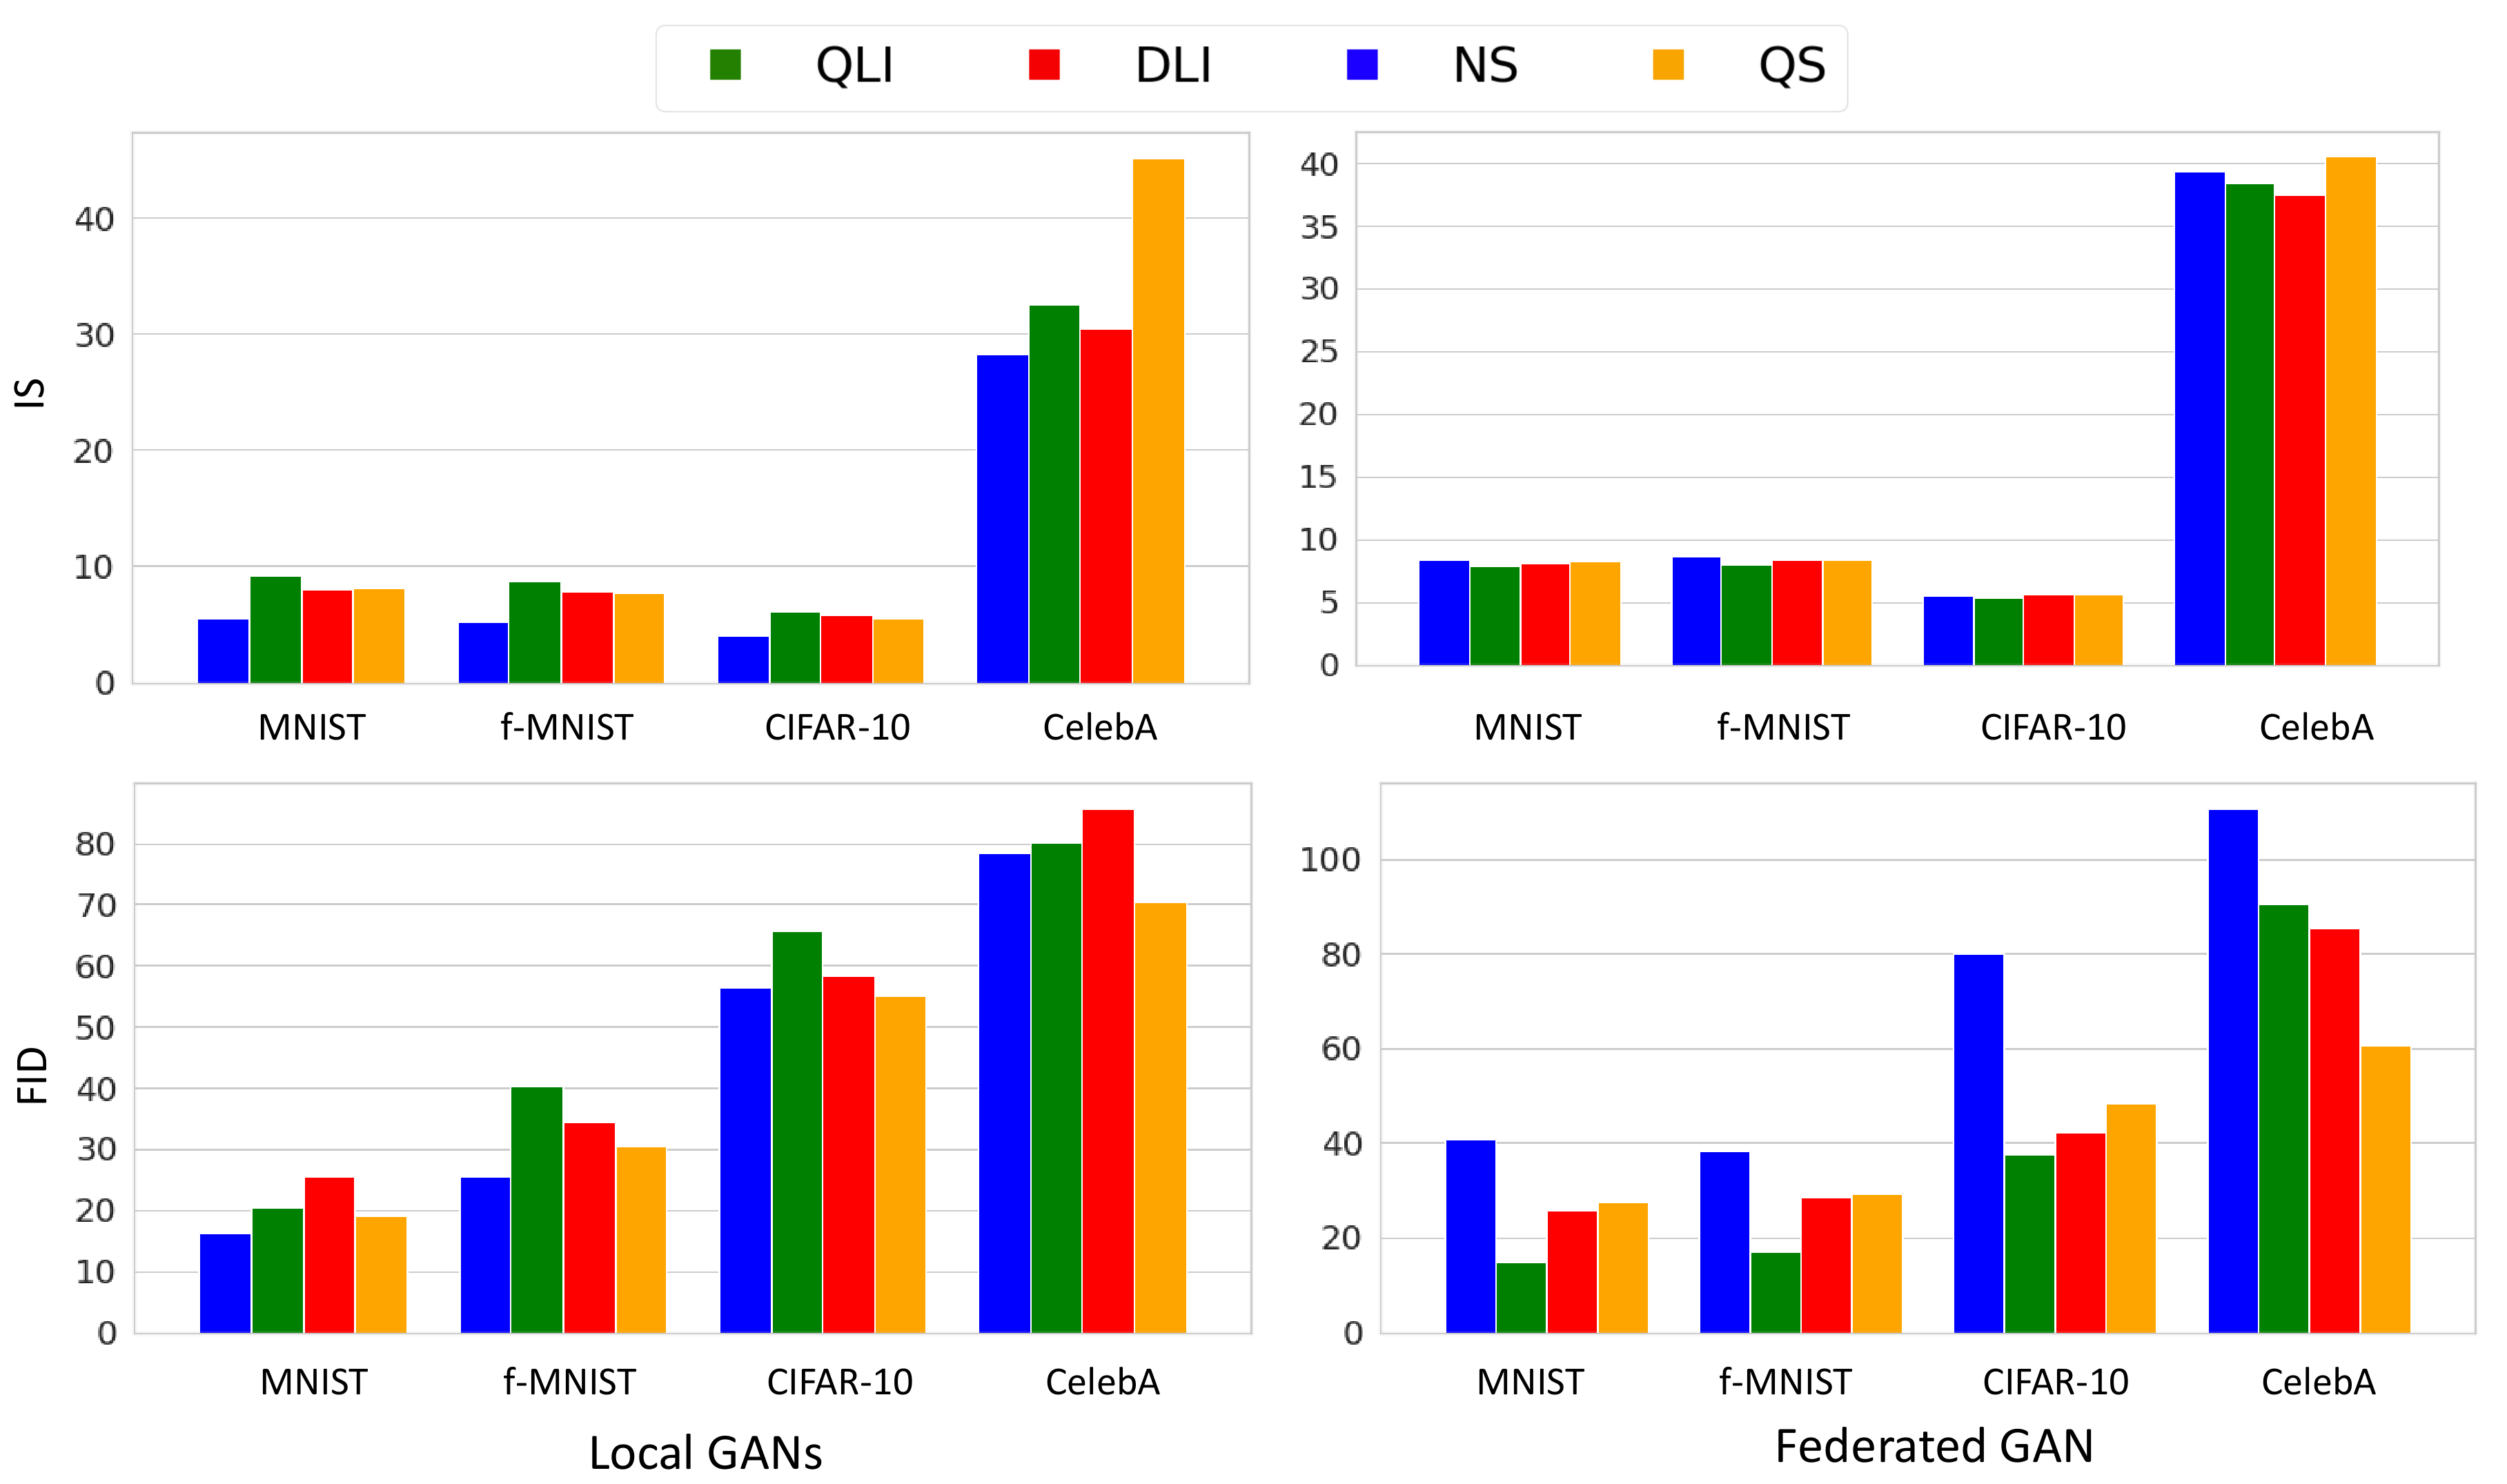
\includegraphics[width=0.7\linewidth]{Plots/baseline_IS_FID.png}
 \caption{Inception Score with Non-Private Local GANs and Federated GAN: The Figure shows the inception score and FID score for different distributions for each dataset in local GANs and federated  GAN with $K=10$. }
 \label{fig:baseline_IS}
\end{figure}








\begin{figure}
 \centering
 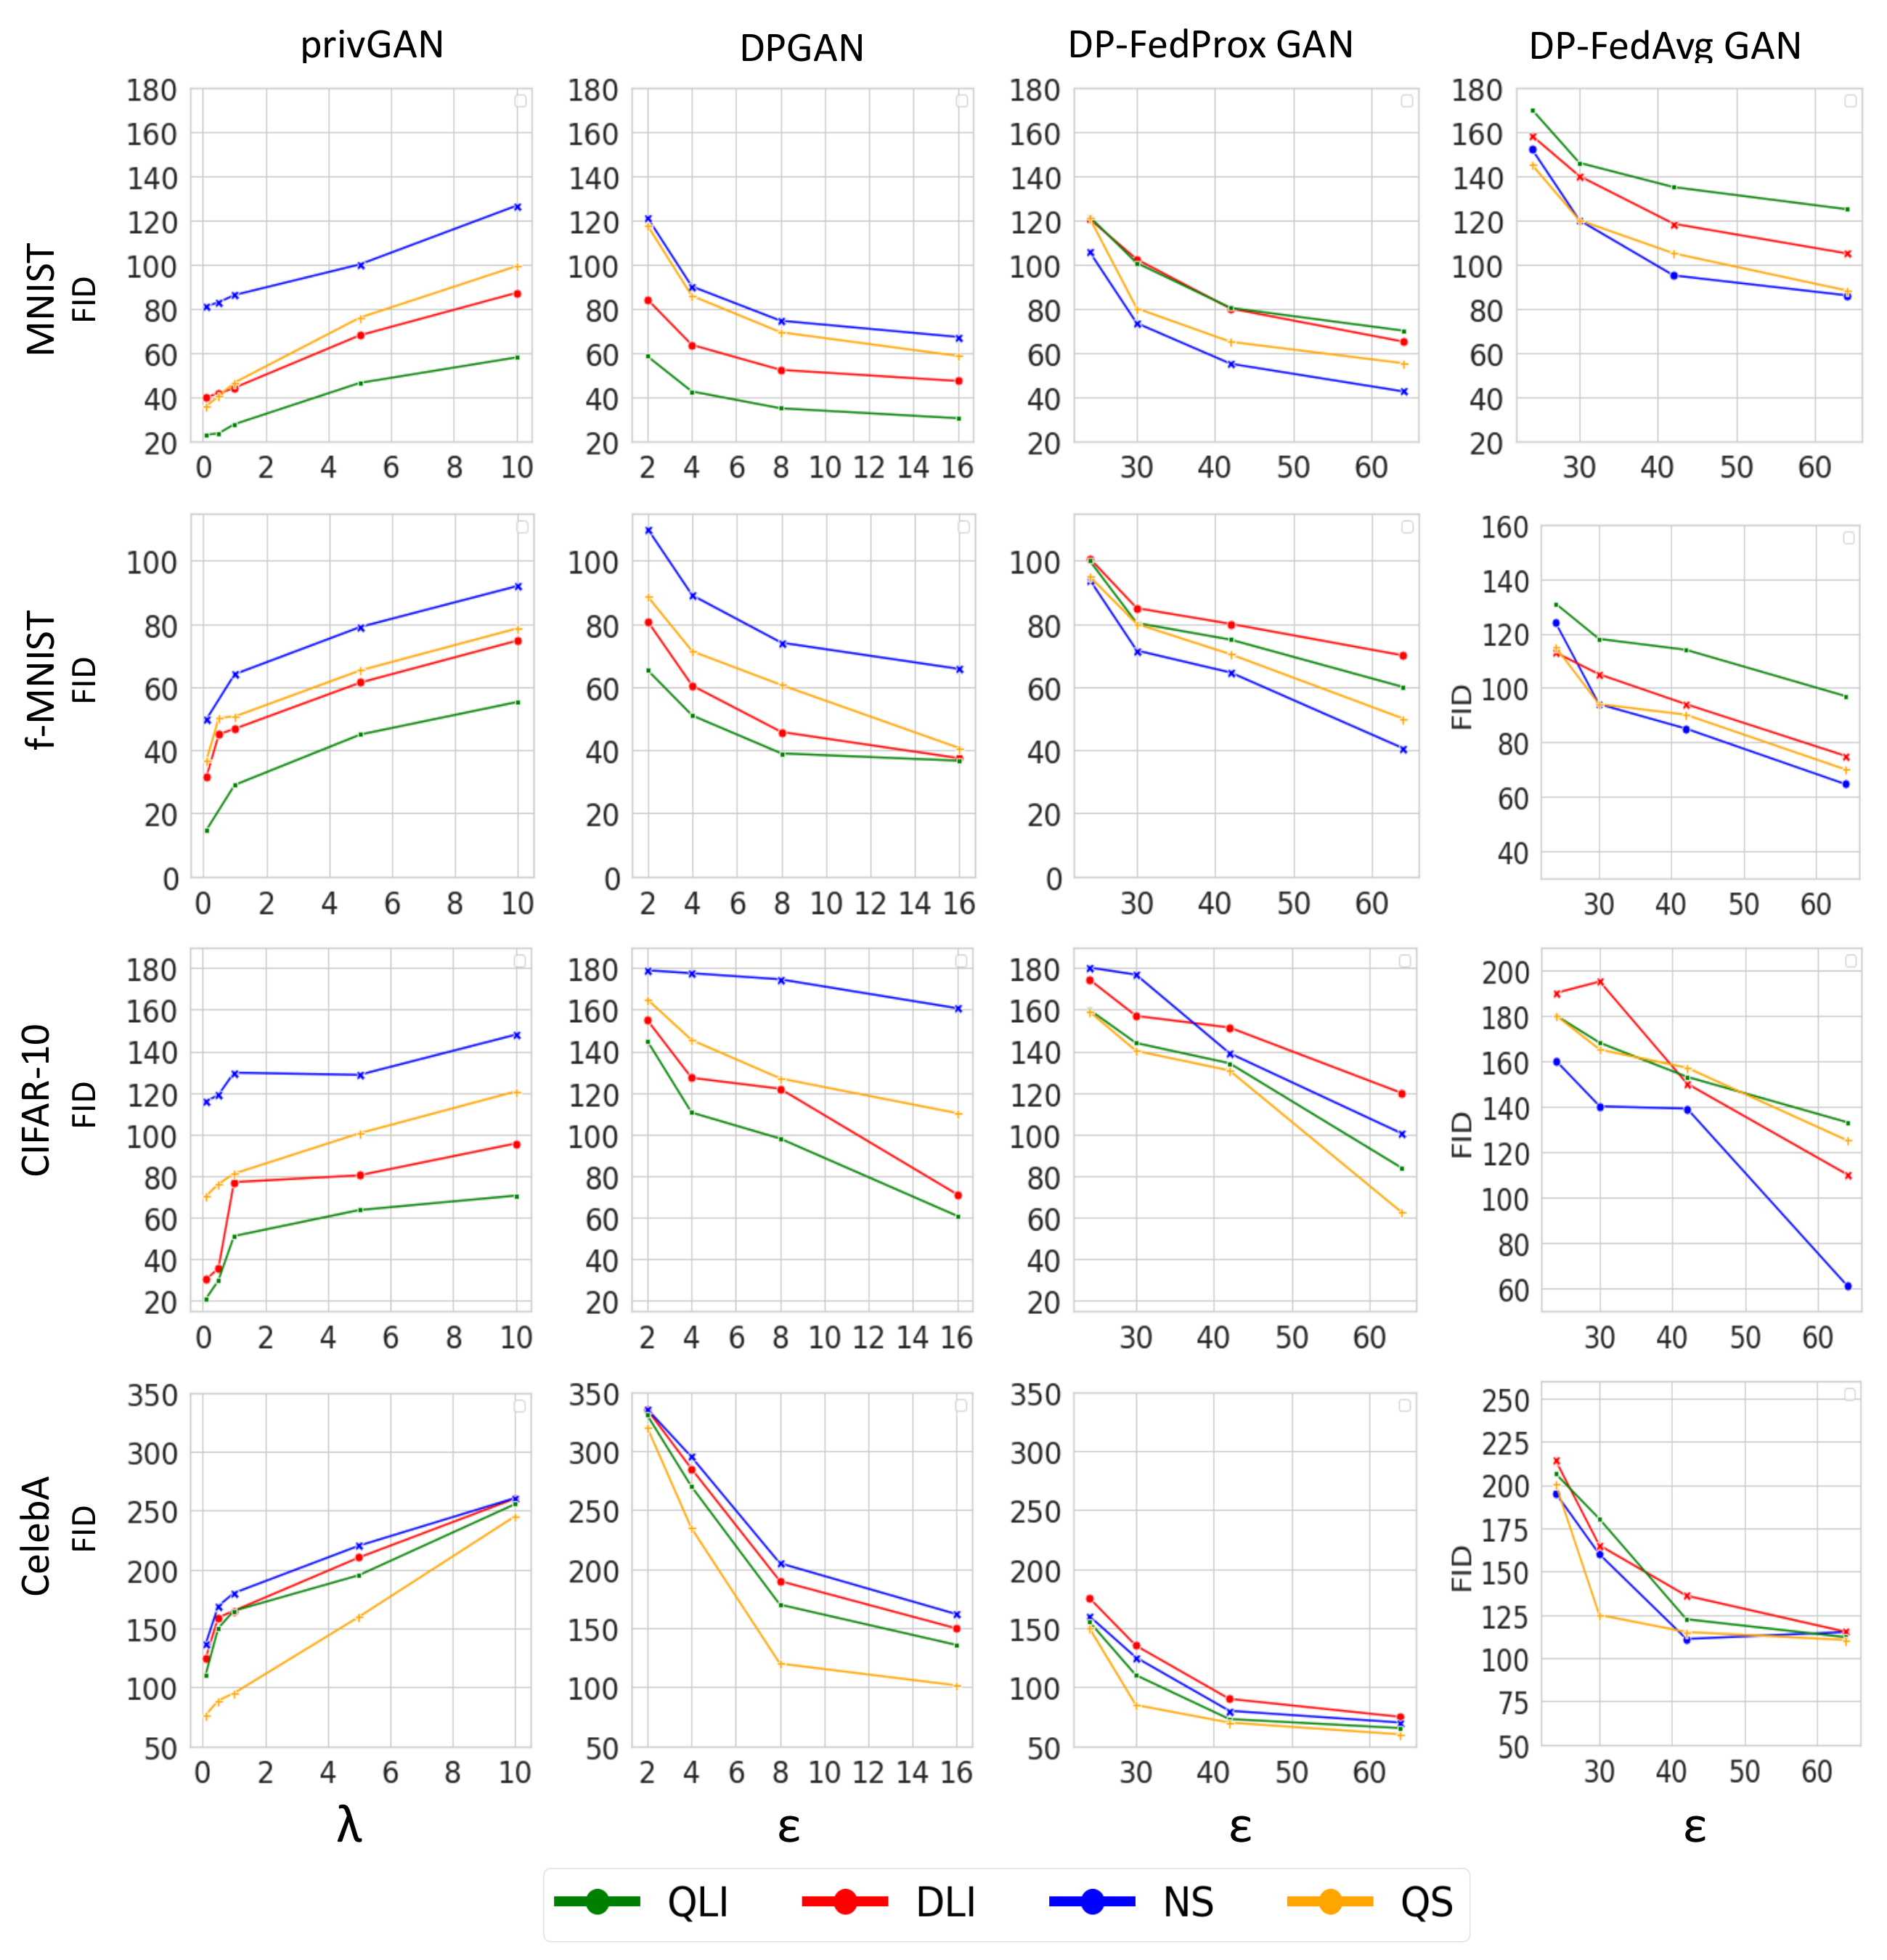
\includegraphics[width=0.8\linewidth]{Plots/vary_privacy_FID.png}
 \caption{Varying Privacy Parameters: The Figure illustrates FID Score for various privacy parameters in privGAN, DPGAN, DP-FedProx GAN, and DP-FedAvg GAN.}
 \label{fig:vary_privacy_FID}
\end{figure}


\begin{figure}
 \centering
 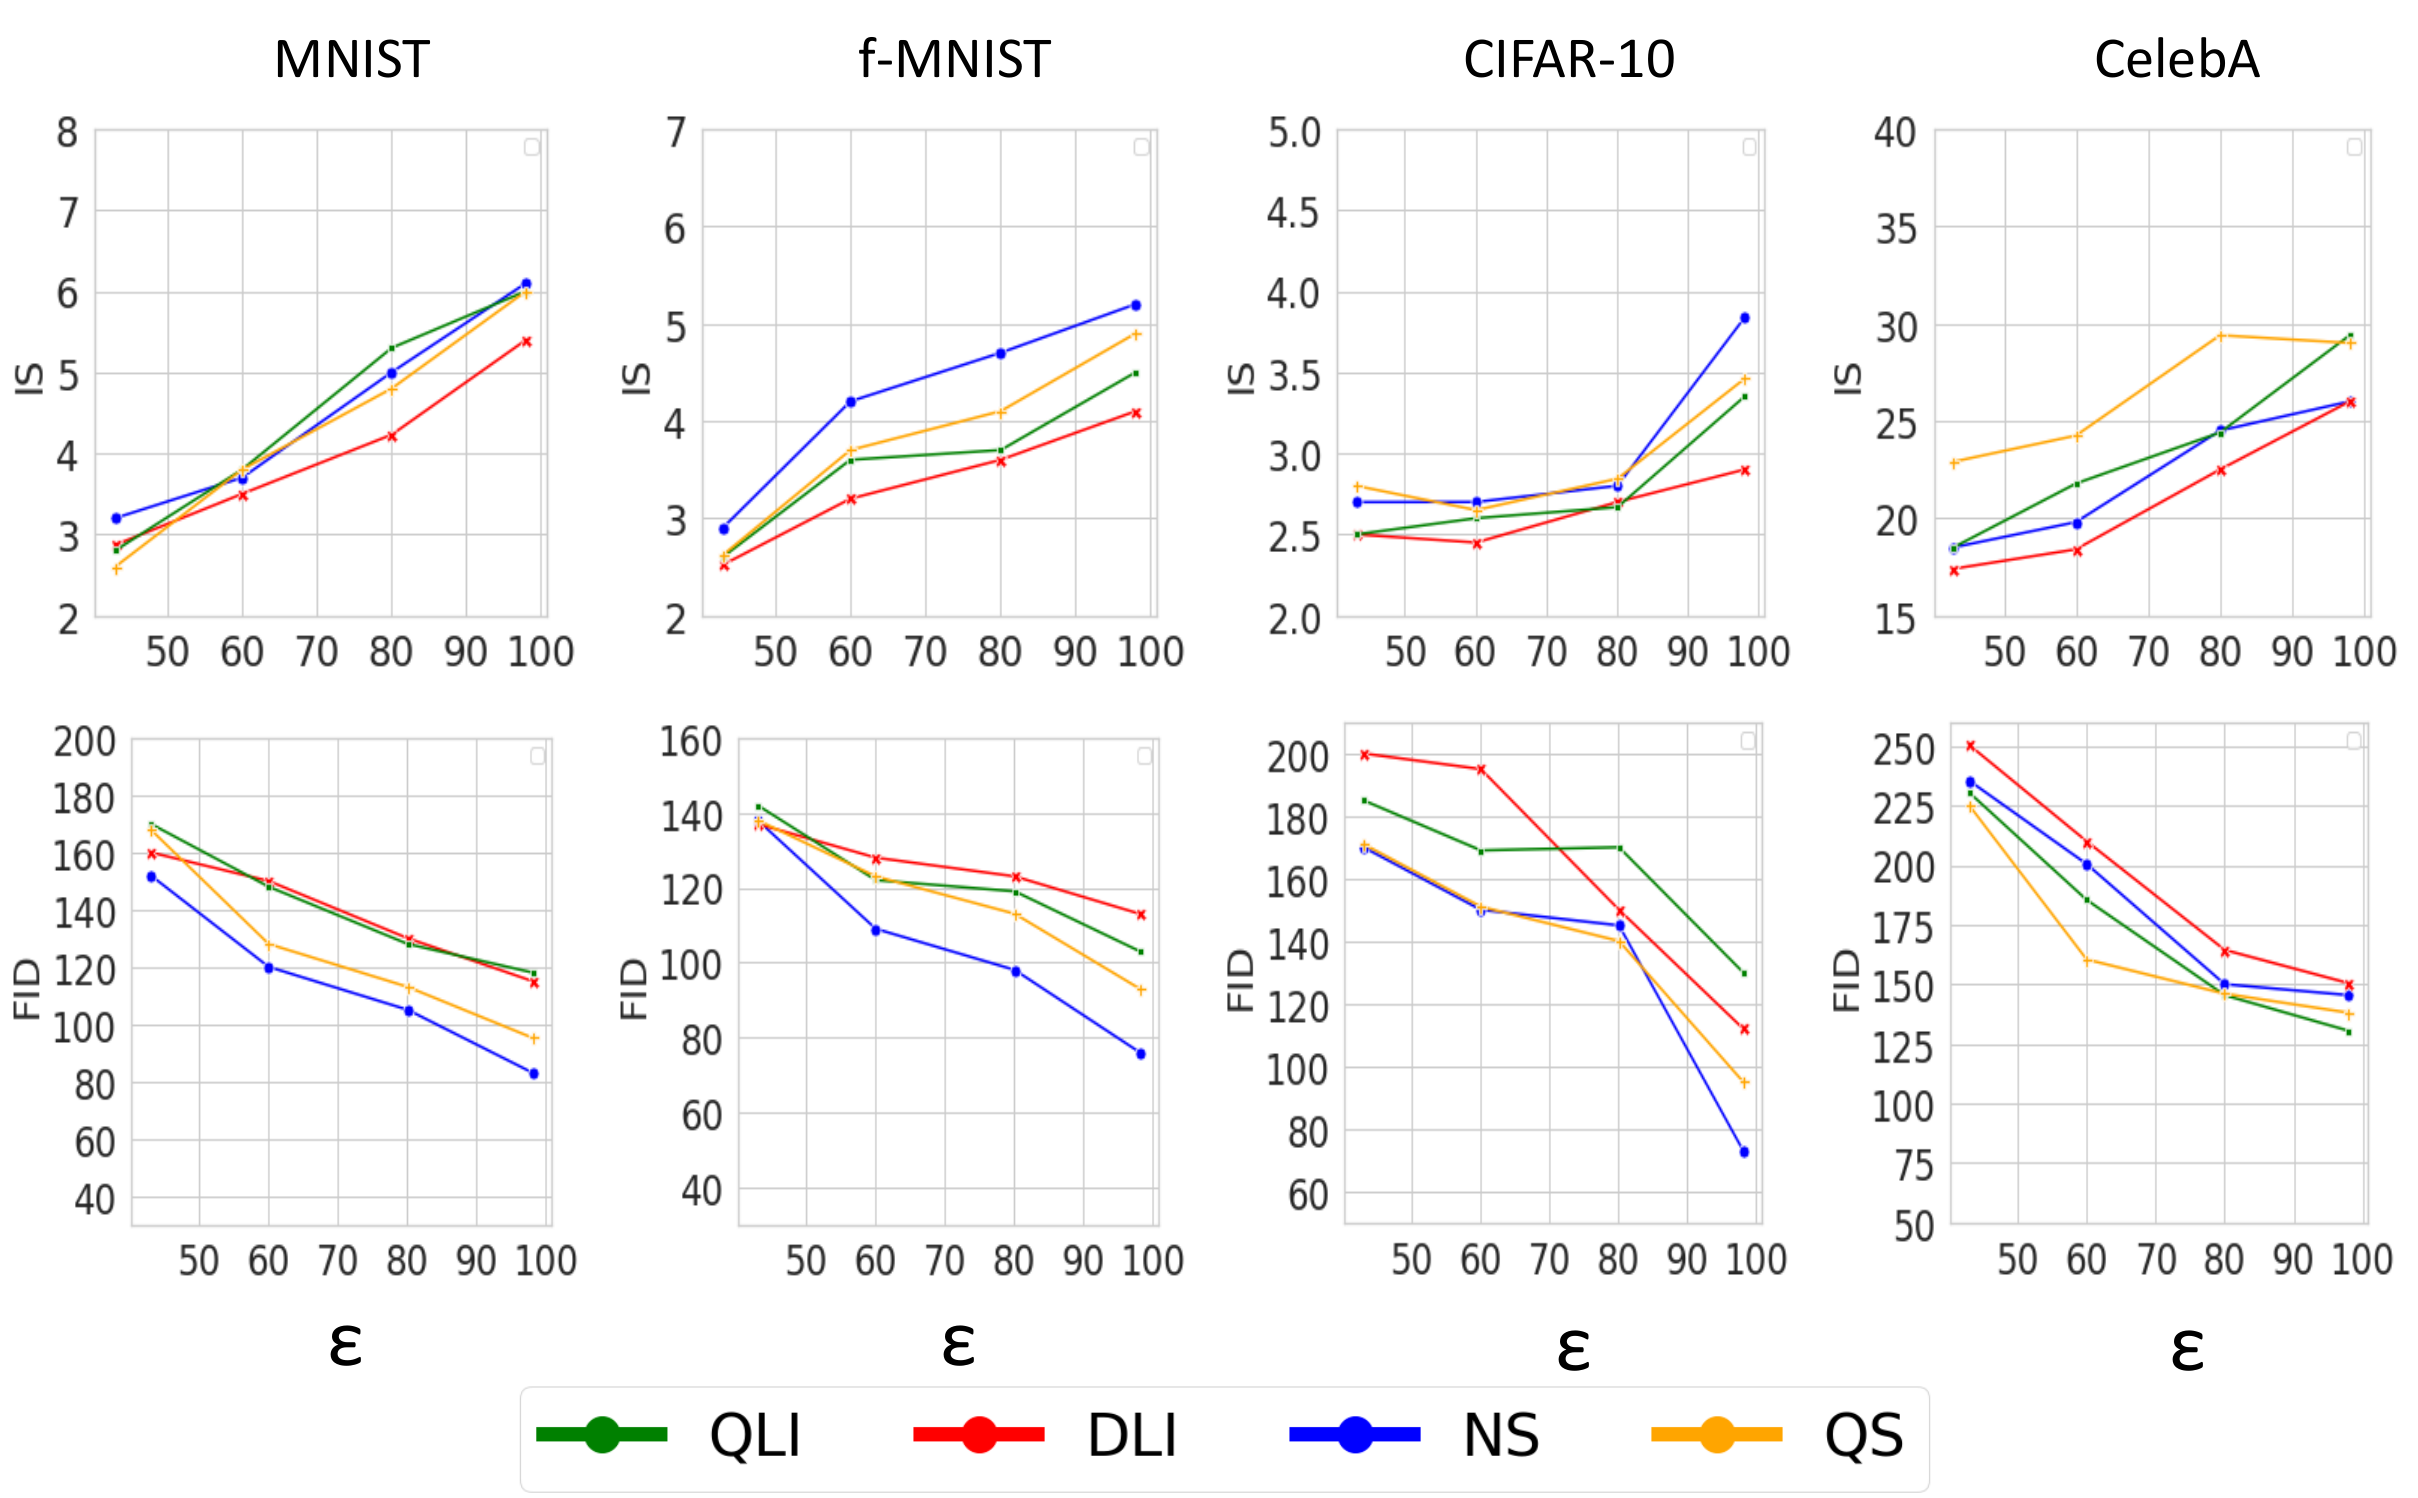
\includegraphics[width=0.8\linewidth]{Plots/vary_privacy_fedsgd.png}
 \caption{Varying Privacy Parameters in DP-FedSGD GAN: The Figure represents inception  and FID Score at various privacy parameters in DP-FedSGD GAN. DP-FedSGD GAN has the worst utility in terms of IS and FID compared to the DP-FedProx GAN and DP-FedAvg GAN, as shown in the Fig~\ref{fig:varyNoise} and ~\ref{fig:vary_privacy_FID}.} 
 \label{fig:vary_privacy_fedsgd}
\end{figure}


\begin{figure}
 \centering
 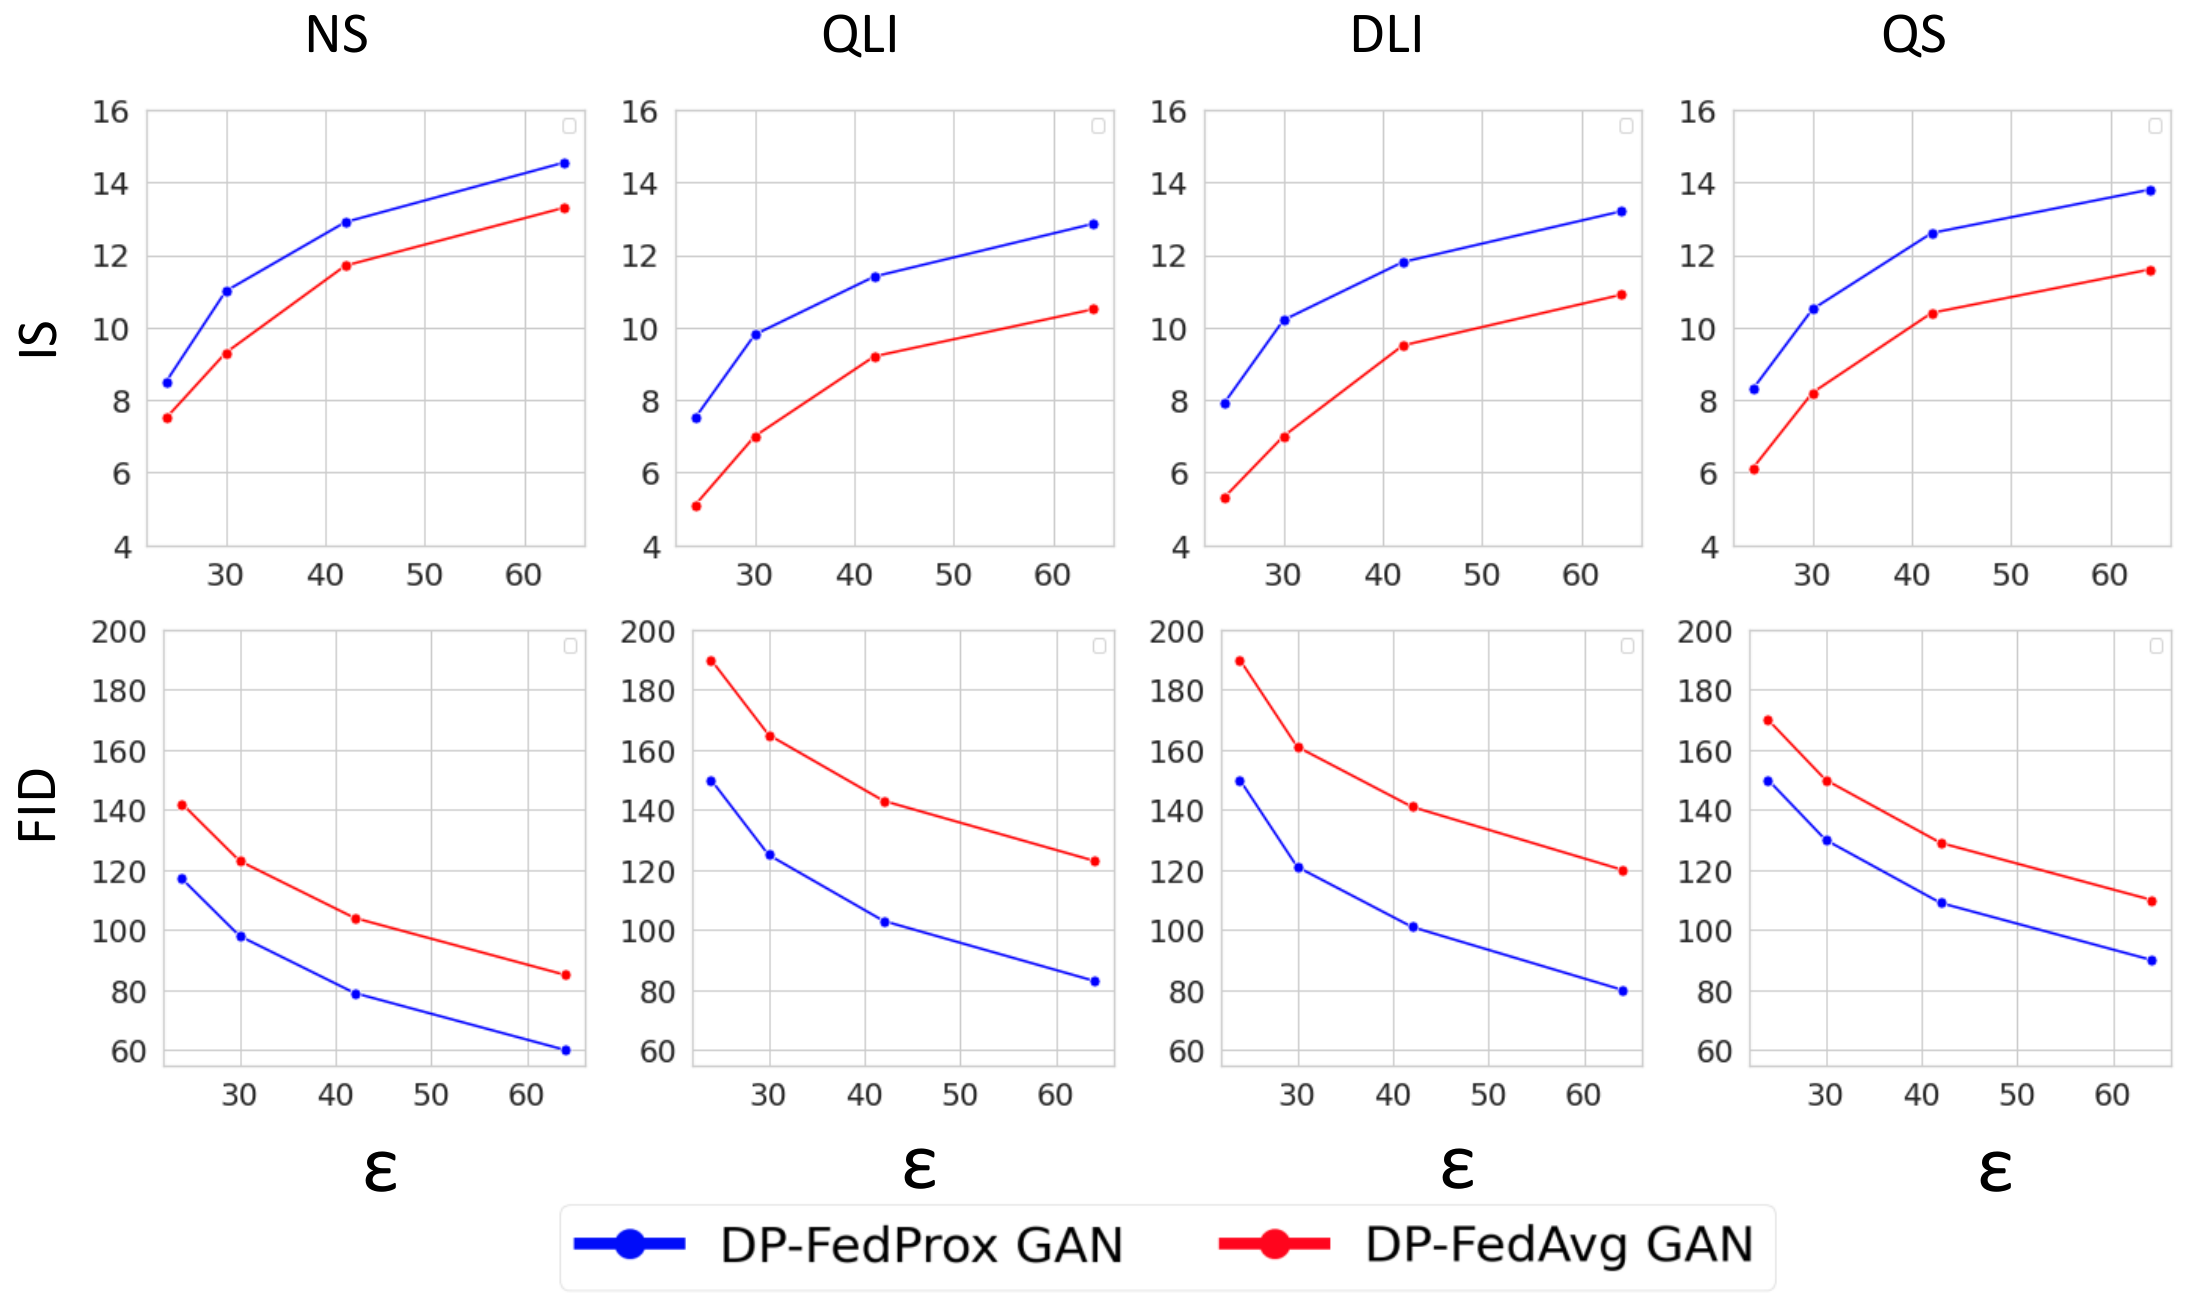
\includegraphics[width=0.7\linewidth]{Plots/varyNoise_emnist.png}
	\caption{\small Varying Privacy Parameters on EMNIST. The Figure depicts the inception and FID score  at various privacy parameters in DP-FedProx GAN and DP-FedAvg GAN at K=500 on EMNIST. }
 \label{fig:varyNoise_emnist}
\end{figure}

\begin{figure}
 \centering
 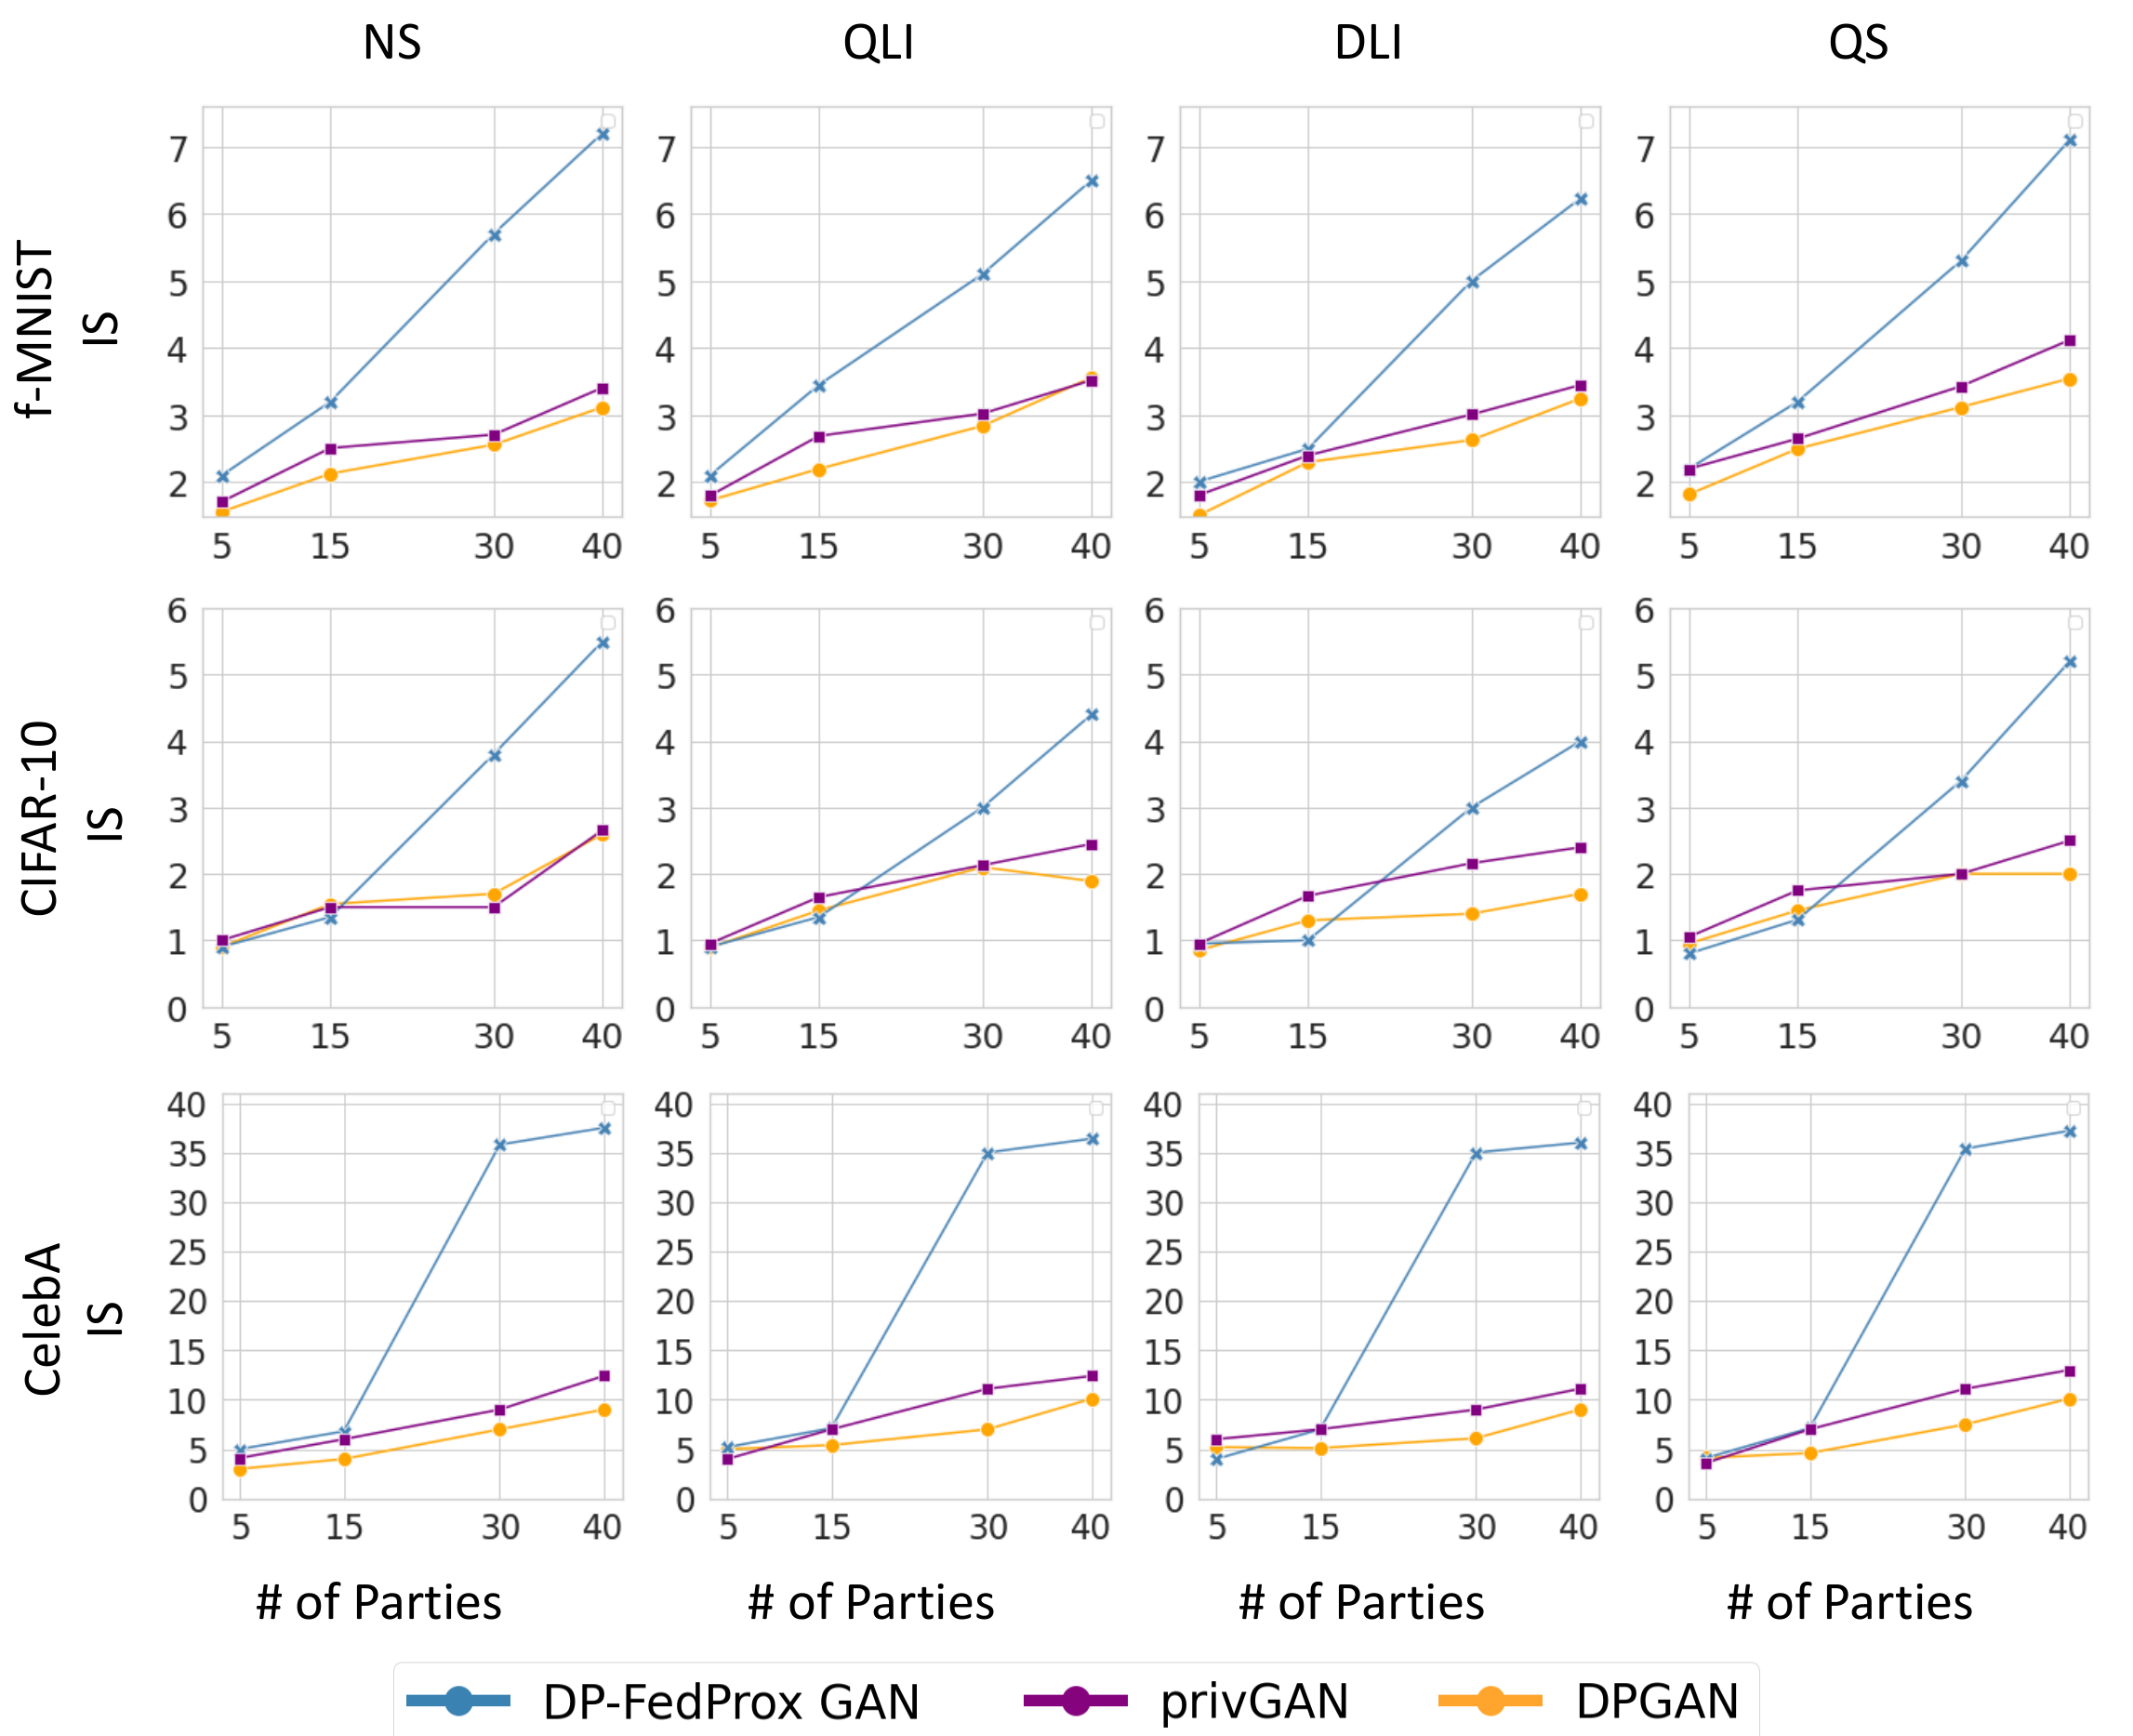
\includegraphics[width=0.8\linewidth]{Plots/vary_parties_IS.png}
 \caption{Varying Number of Parties: The Figure depicts the inception score for various distributions at various numbers of parties in privGAN, DPGAN, and DP-FedProx GAN.}

 
 \label{fig:vary_parties_IS}
\end{figure}



% \begin{figure}
%  \centering
%  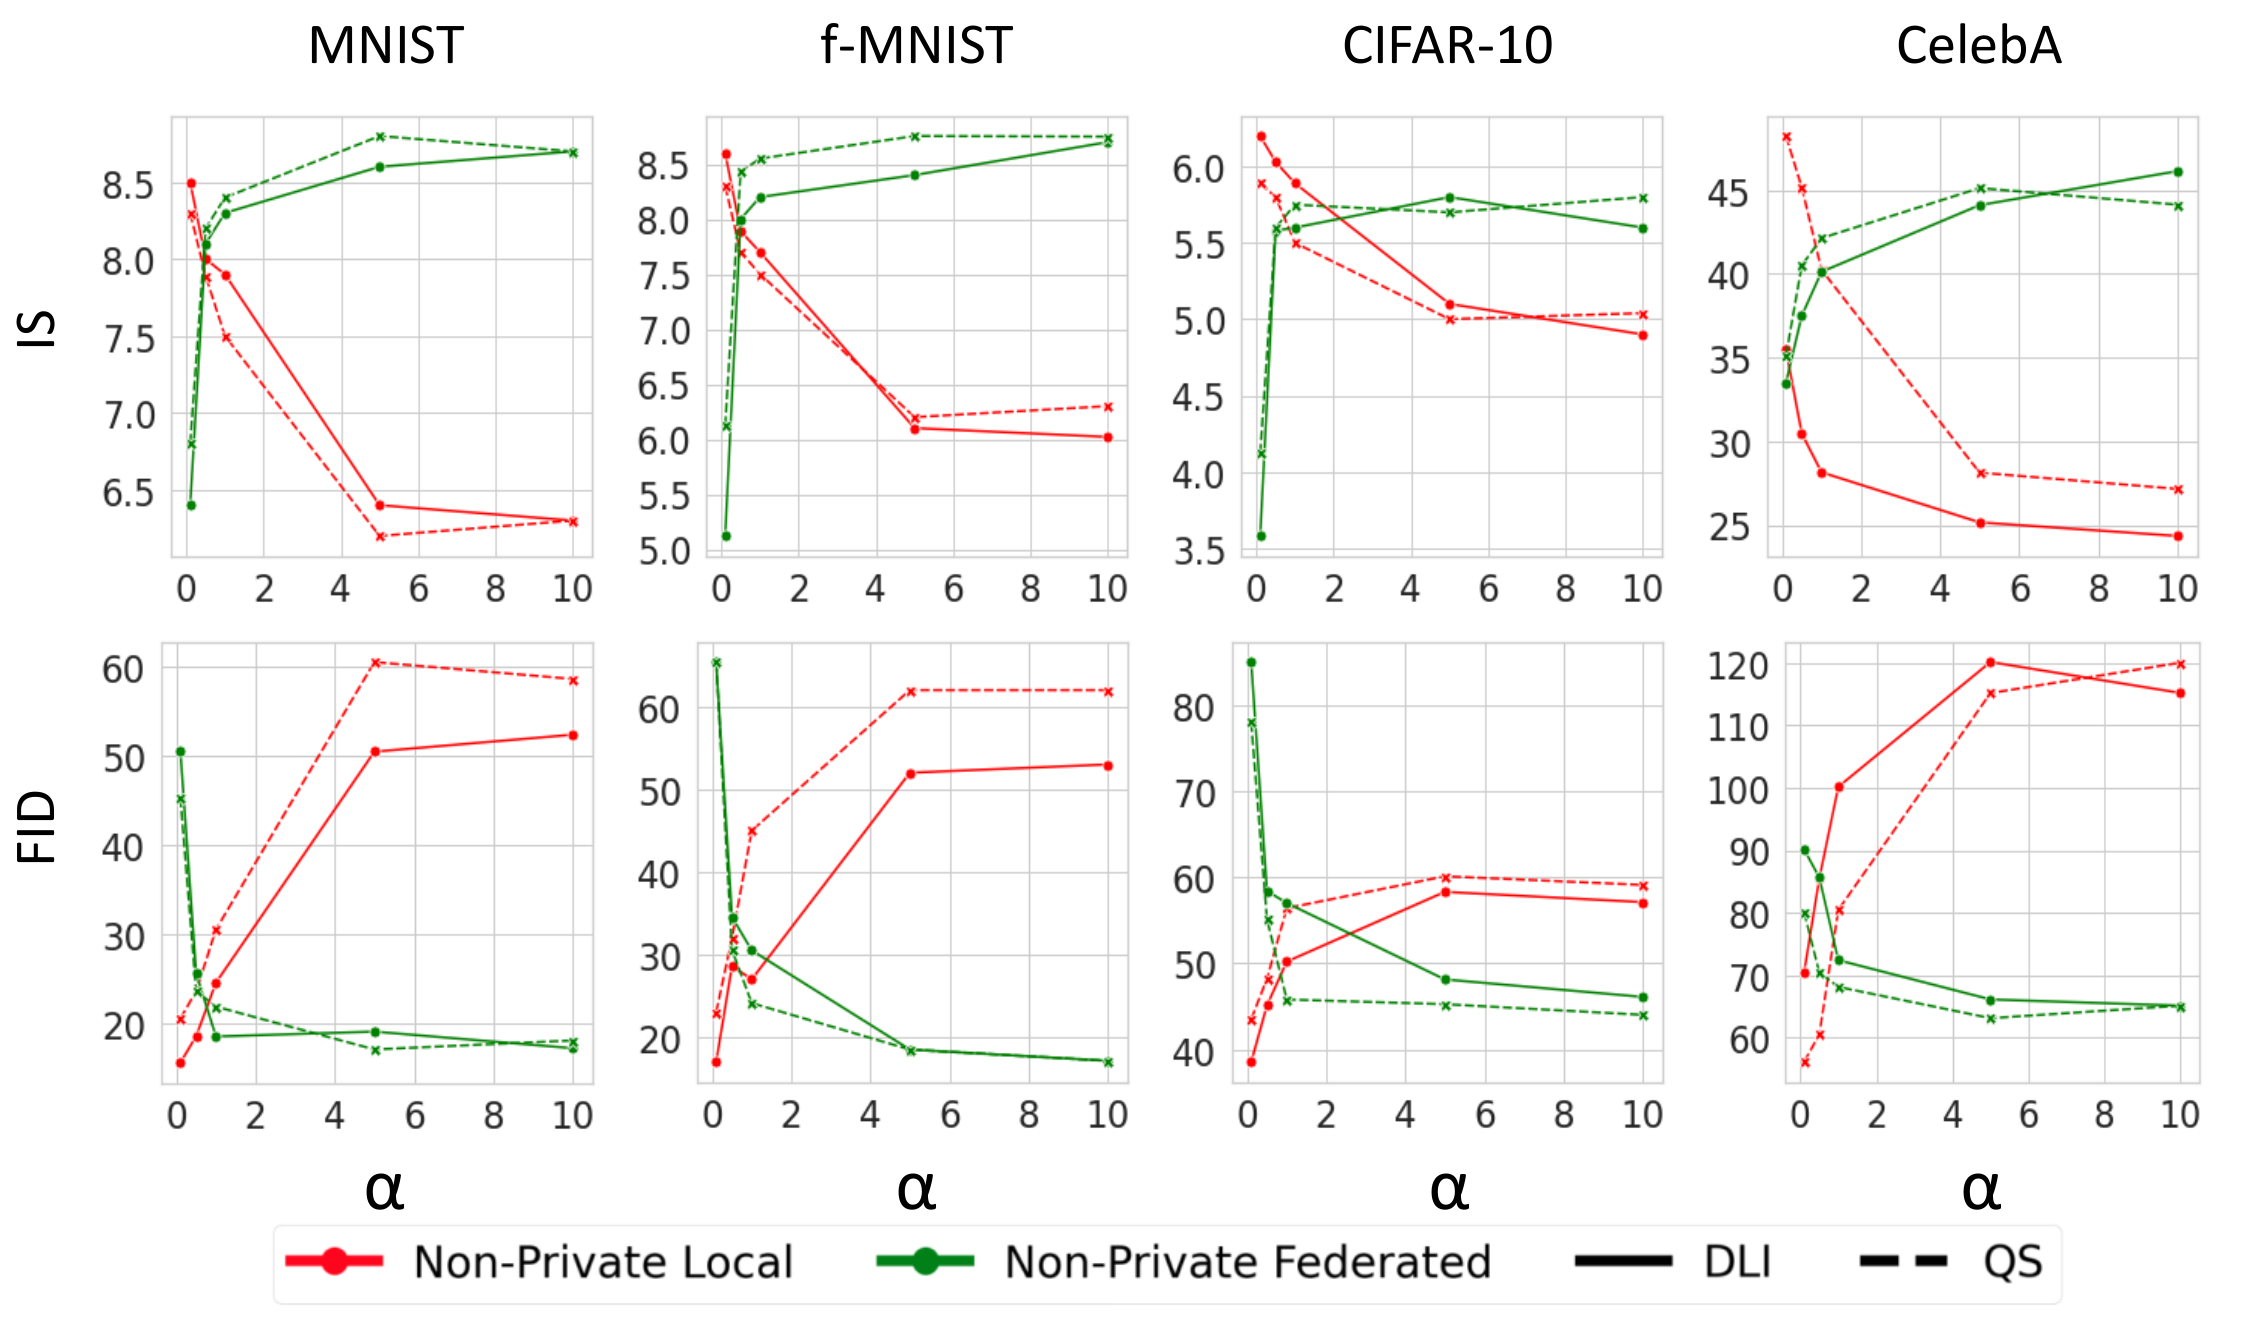
\includegraphics[width=0.8\linewidth]{Plots/nonprivate_vary_alpha_utility.png}
%  \caption{Varying Concentration Parameter for Non-Private Local GANs and Federated GAN: The Figure shows the inception and FID score for different distributions at various concentration parameters in local GANs and federated  GAN with $K=10$. }
%  \label{fig:nonprivate_vary_alpha_utility}
% \end{figure}

\begin{figure}
 \centering
 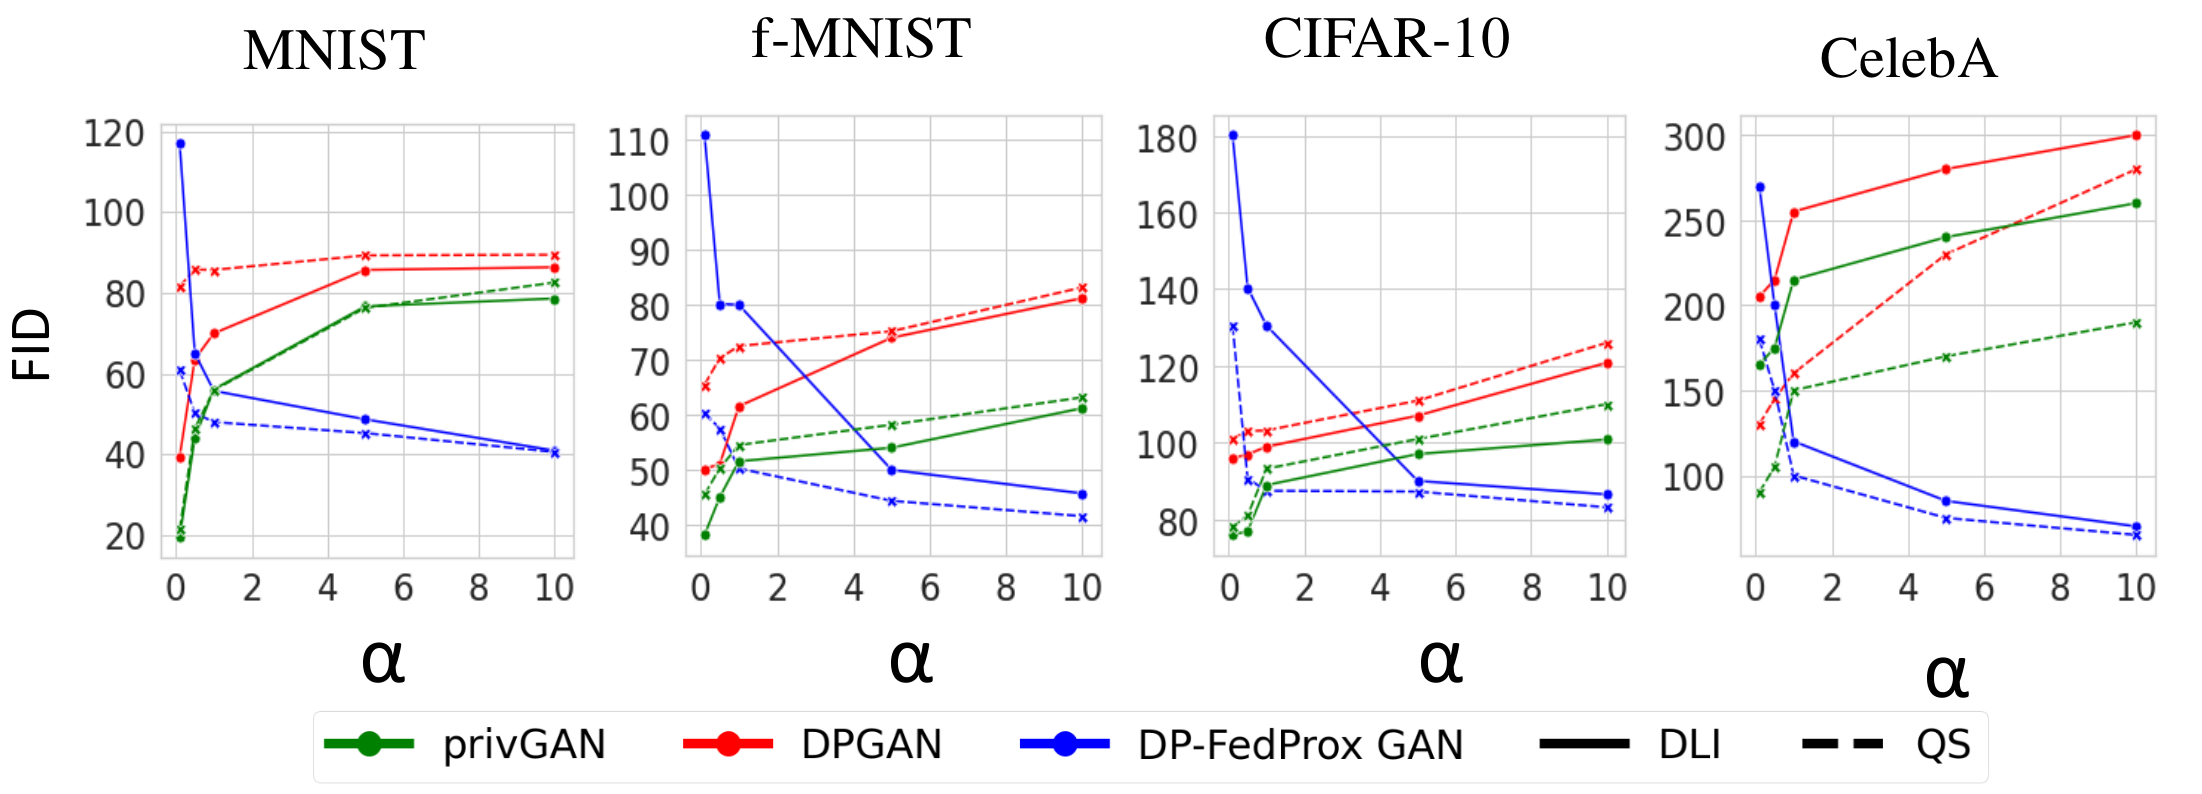
\includegraphics[width=0.8\linewidth]{Plots/vary_alpha_FID.png}
 \caption{Varying Concentration Parameters: The Figure illustrates the FID score for different distributions at various concentration parameters in privGAN, DPGAN, and DP-FedProx GAN. }
 \label{fig:vary_alpha_FID}
\end{figure}




% \begin{figure}
%  \centering
%  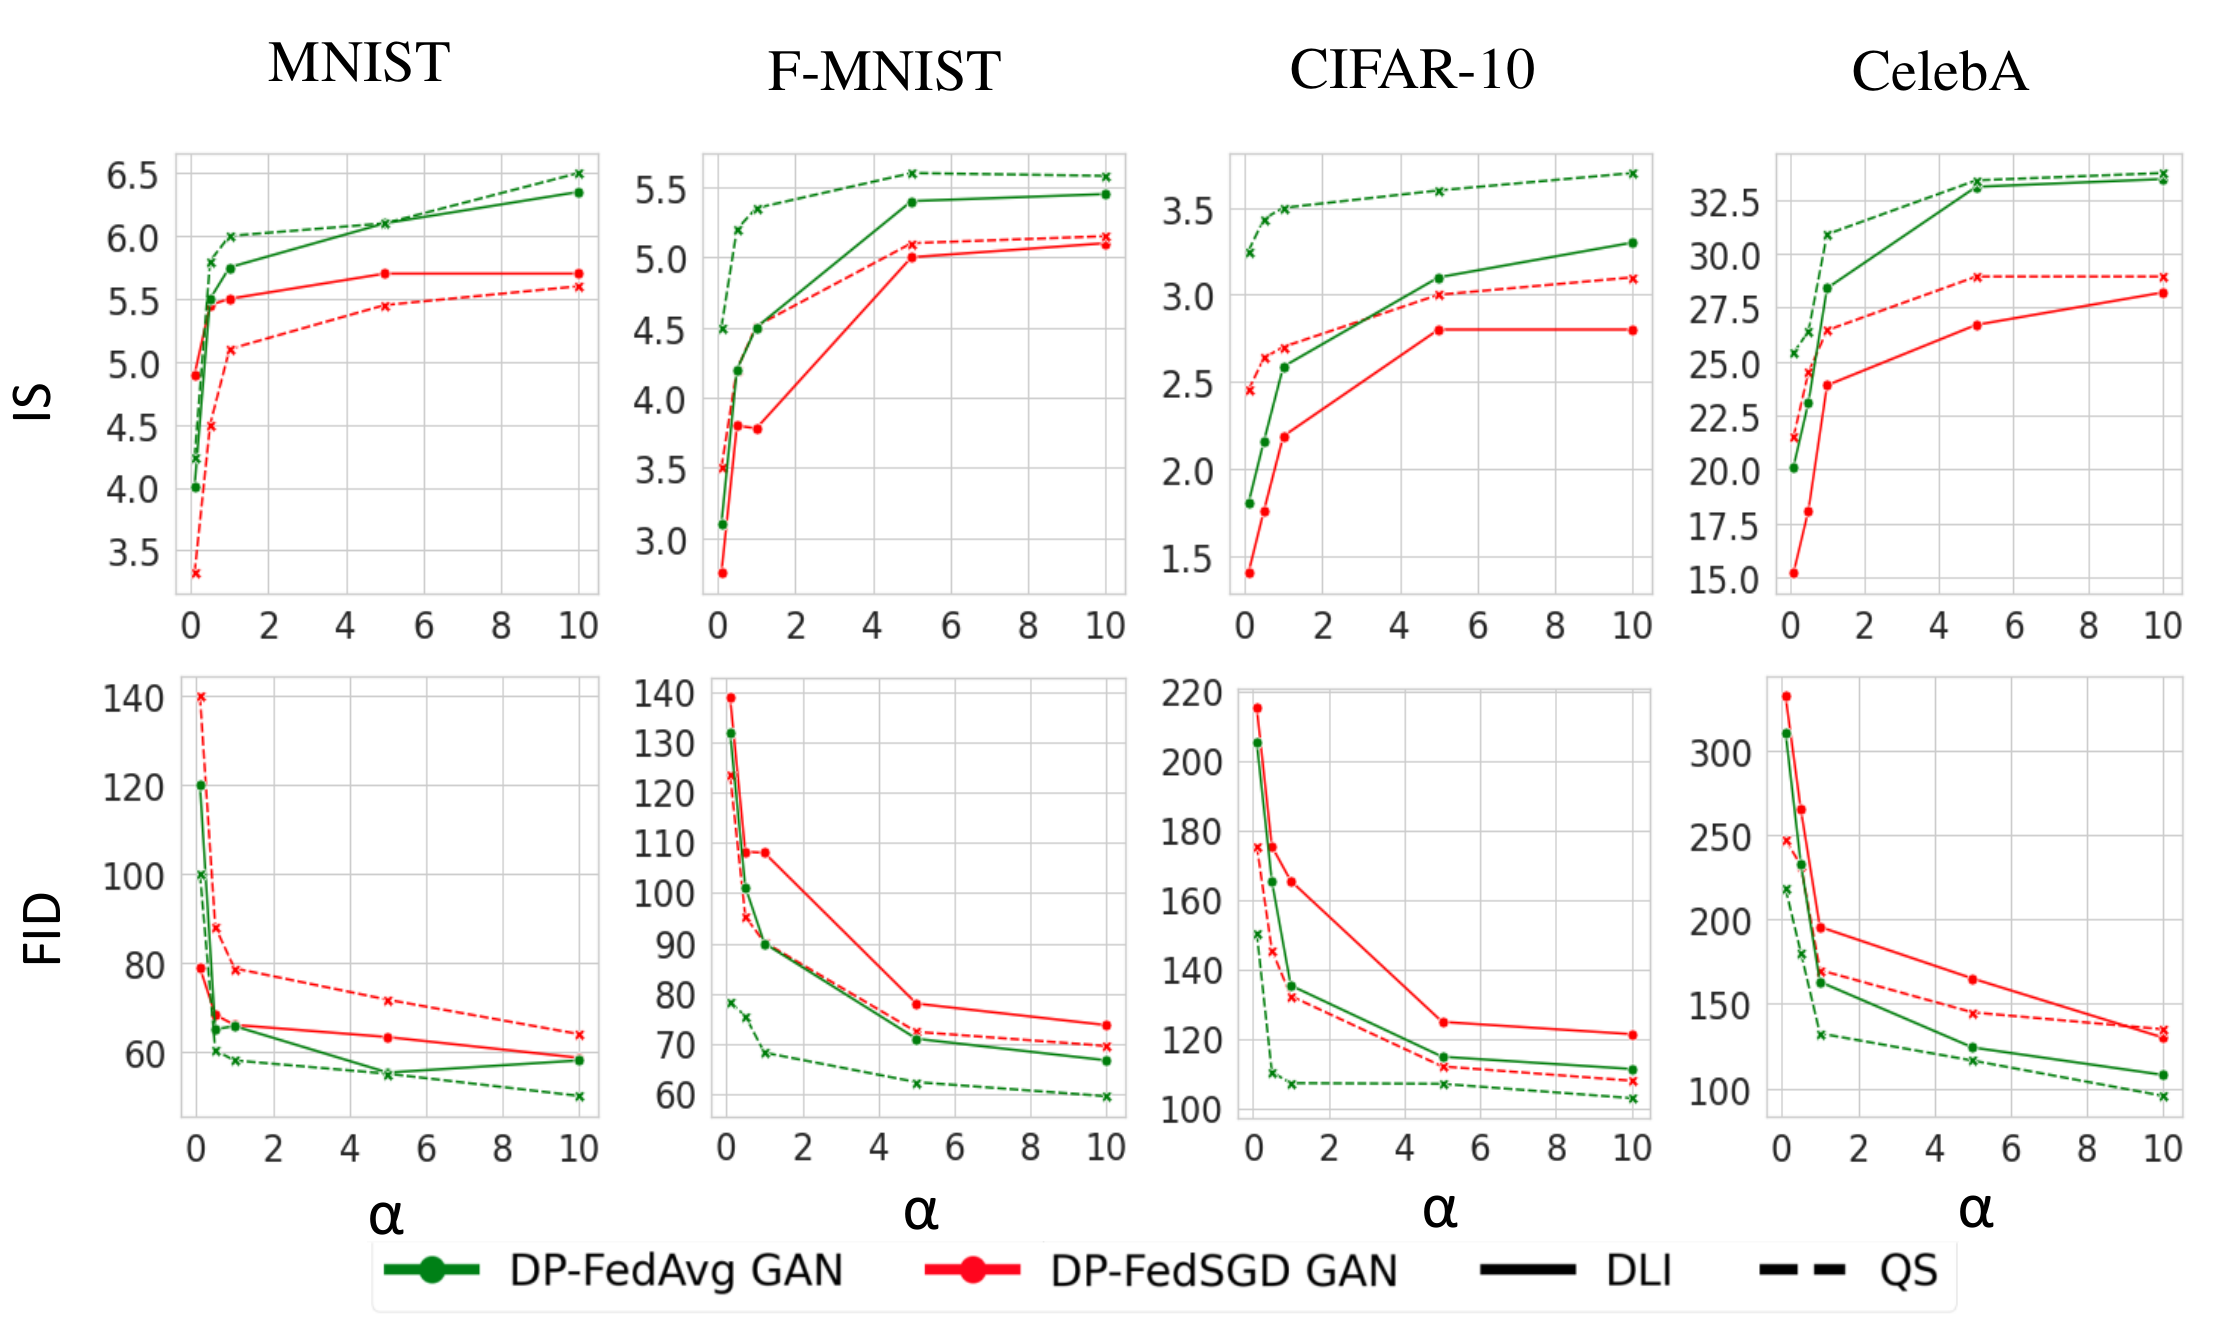
\includegraphics[width=0.8\linewidth]{Plots/vary_alpha_fedsgd_fedavg.png}
%  \caption{Varying Concentration Parameters in DP-FedAvg GAN and DP-FedSGD GAN: The Figure displays the inception and FID score for various distributions at various concentration parameters in the DP-FedAvg GAN and the DP-FedSGD GAN models.}
%  \label{fig:vary_alpha_fedsgd_fedavg}
% \end{figure}




\begin{figure}
 \centering
 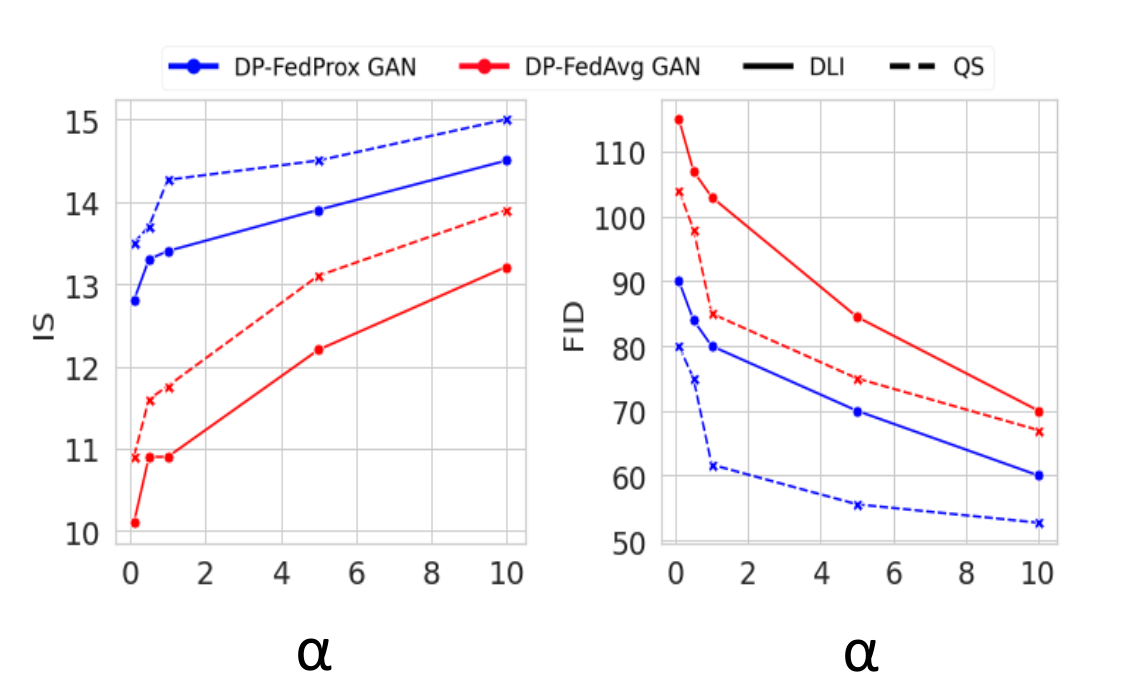
\includegraphics[width=0.45\linewidth]{Plots/varyAlpha_emnist.png}
	\caption{\small Varying Concentration Parameter on EMNIST with 500 Parties ($K$=500) using DP-FedProx GAN  and DP-FedAvg GAN .}
 \label{fig:varyAlpha_emnist}
\end{figure}


% \begin{figure}
%  \centering
%  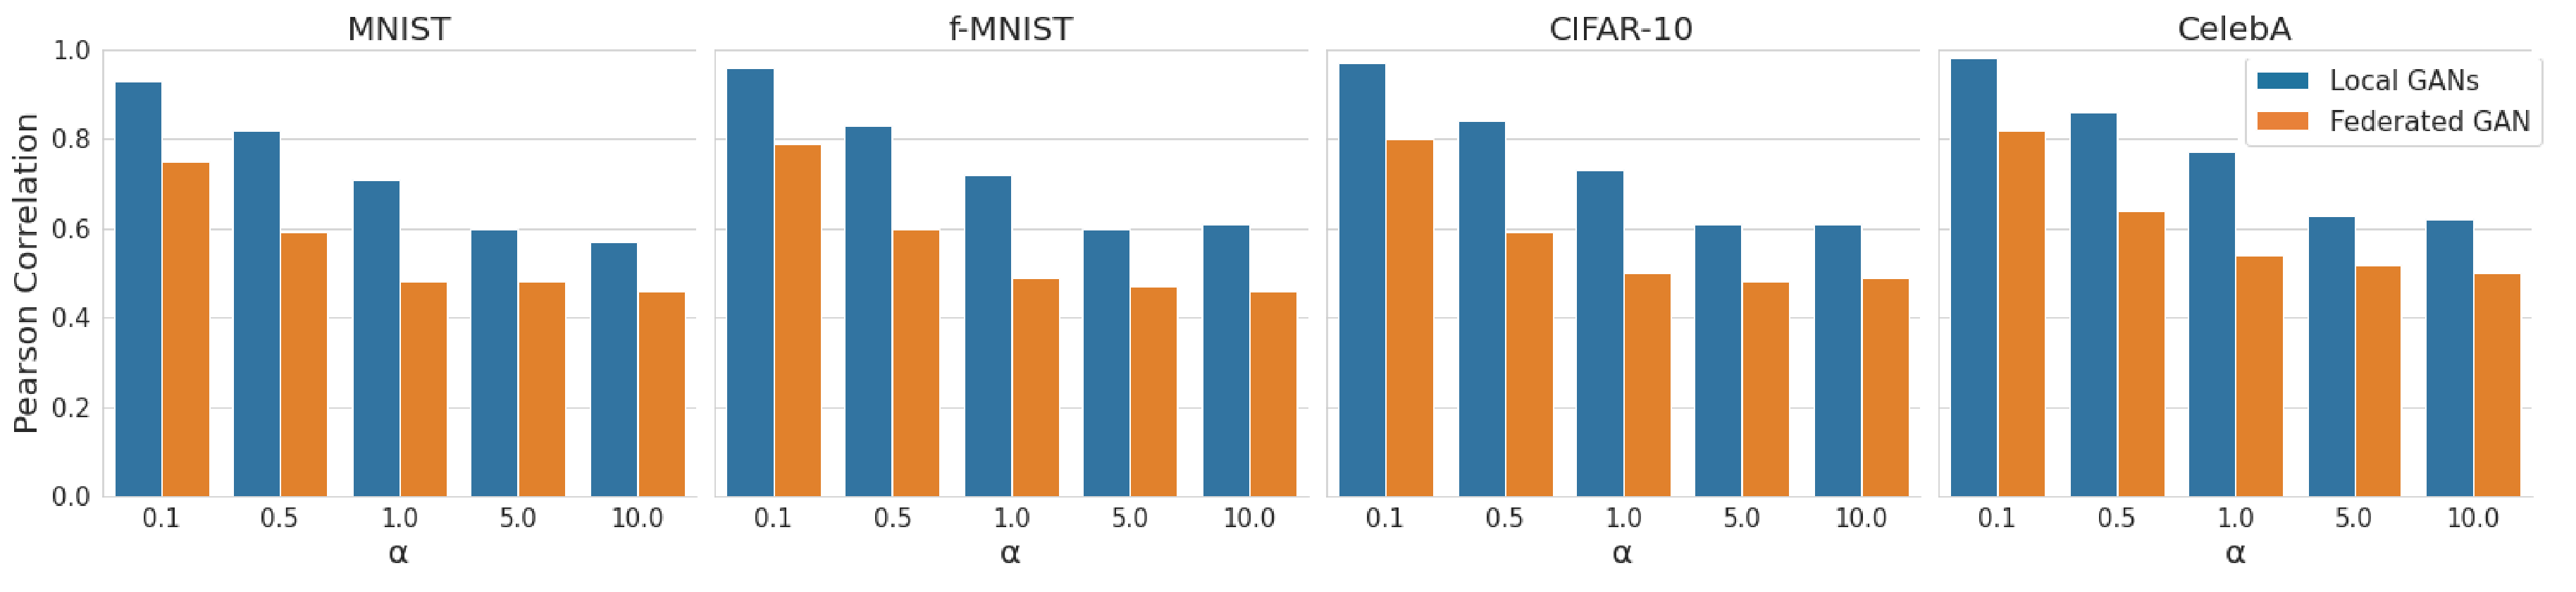
\includegraphics[width=0.8\linewidth]{Plots/IS_alpha_nonprivate.png}
%  \caption{Vary Concentration Parameters in QS distribution: The Figure depicts Pearson correlation $r$ between local data size and local IS at various concentration parameters $\alpha$ in Local GANs and Federated GAN at $K=10$. The correlation in Federated GAN cannot be evaluated directly due to synthetic samples provided by the central server. For the Federated GAN, we evaluated each local party's impact on overall IS by calculating the difference in IS when all parties' data was utilized versus excluding the data from a specific local party.  }
%  \label{fig:IS_alpha_nonprivate}
% \end{figure}



% \begin{figure}
%  \centering
%  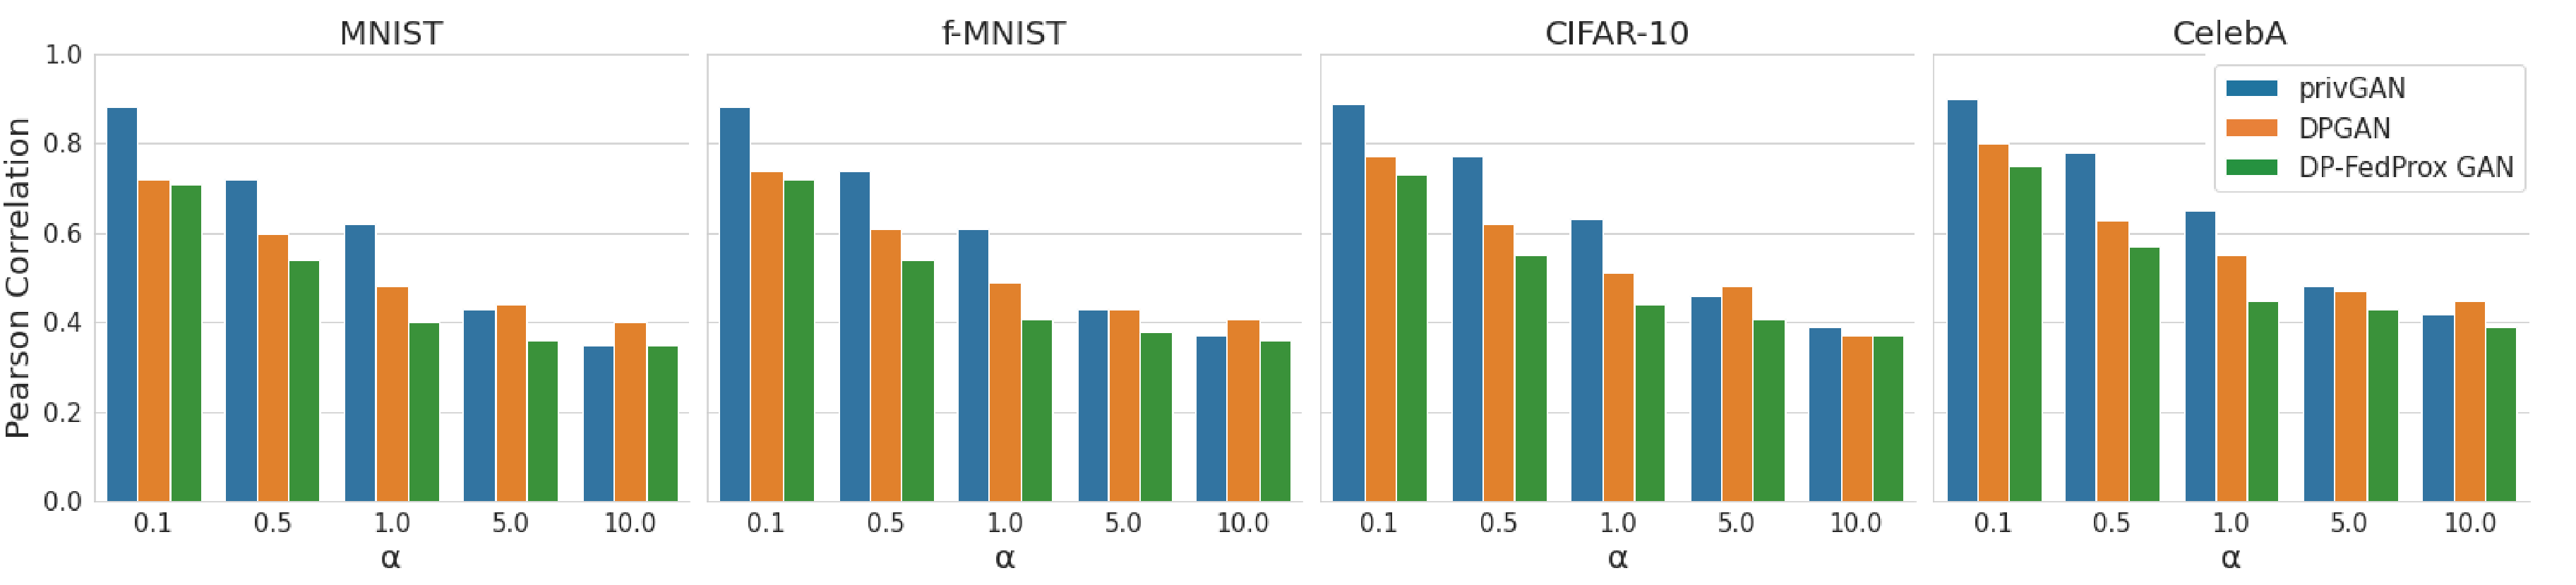
\includegraphics[width=0.8\linewidth]{Plots/IS_alpha_private.png}
%  \caption{Vary Concentration Parameters in QS distribution: The Figure depicts Pearson correlation $r$ between local data size and local IS at various concentration parameters $\alpha$ in privGAN, DPGAN,  and DP-FedProx GAN. For the DP-FedProx GAN, we evaluated each local party's impact on overall IS by calculating the difference in IS when all parties' data was utilized versus excluding the data from a specific local party.  }
%  \label{fig:IS_alpha_private}
% \end{figure}


% \begin{figure}
%  \centering
%  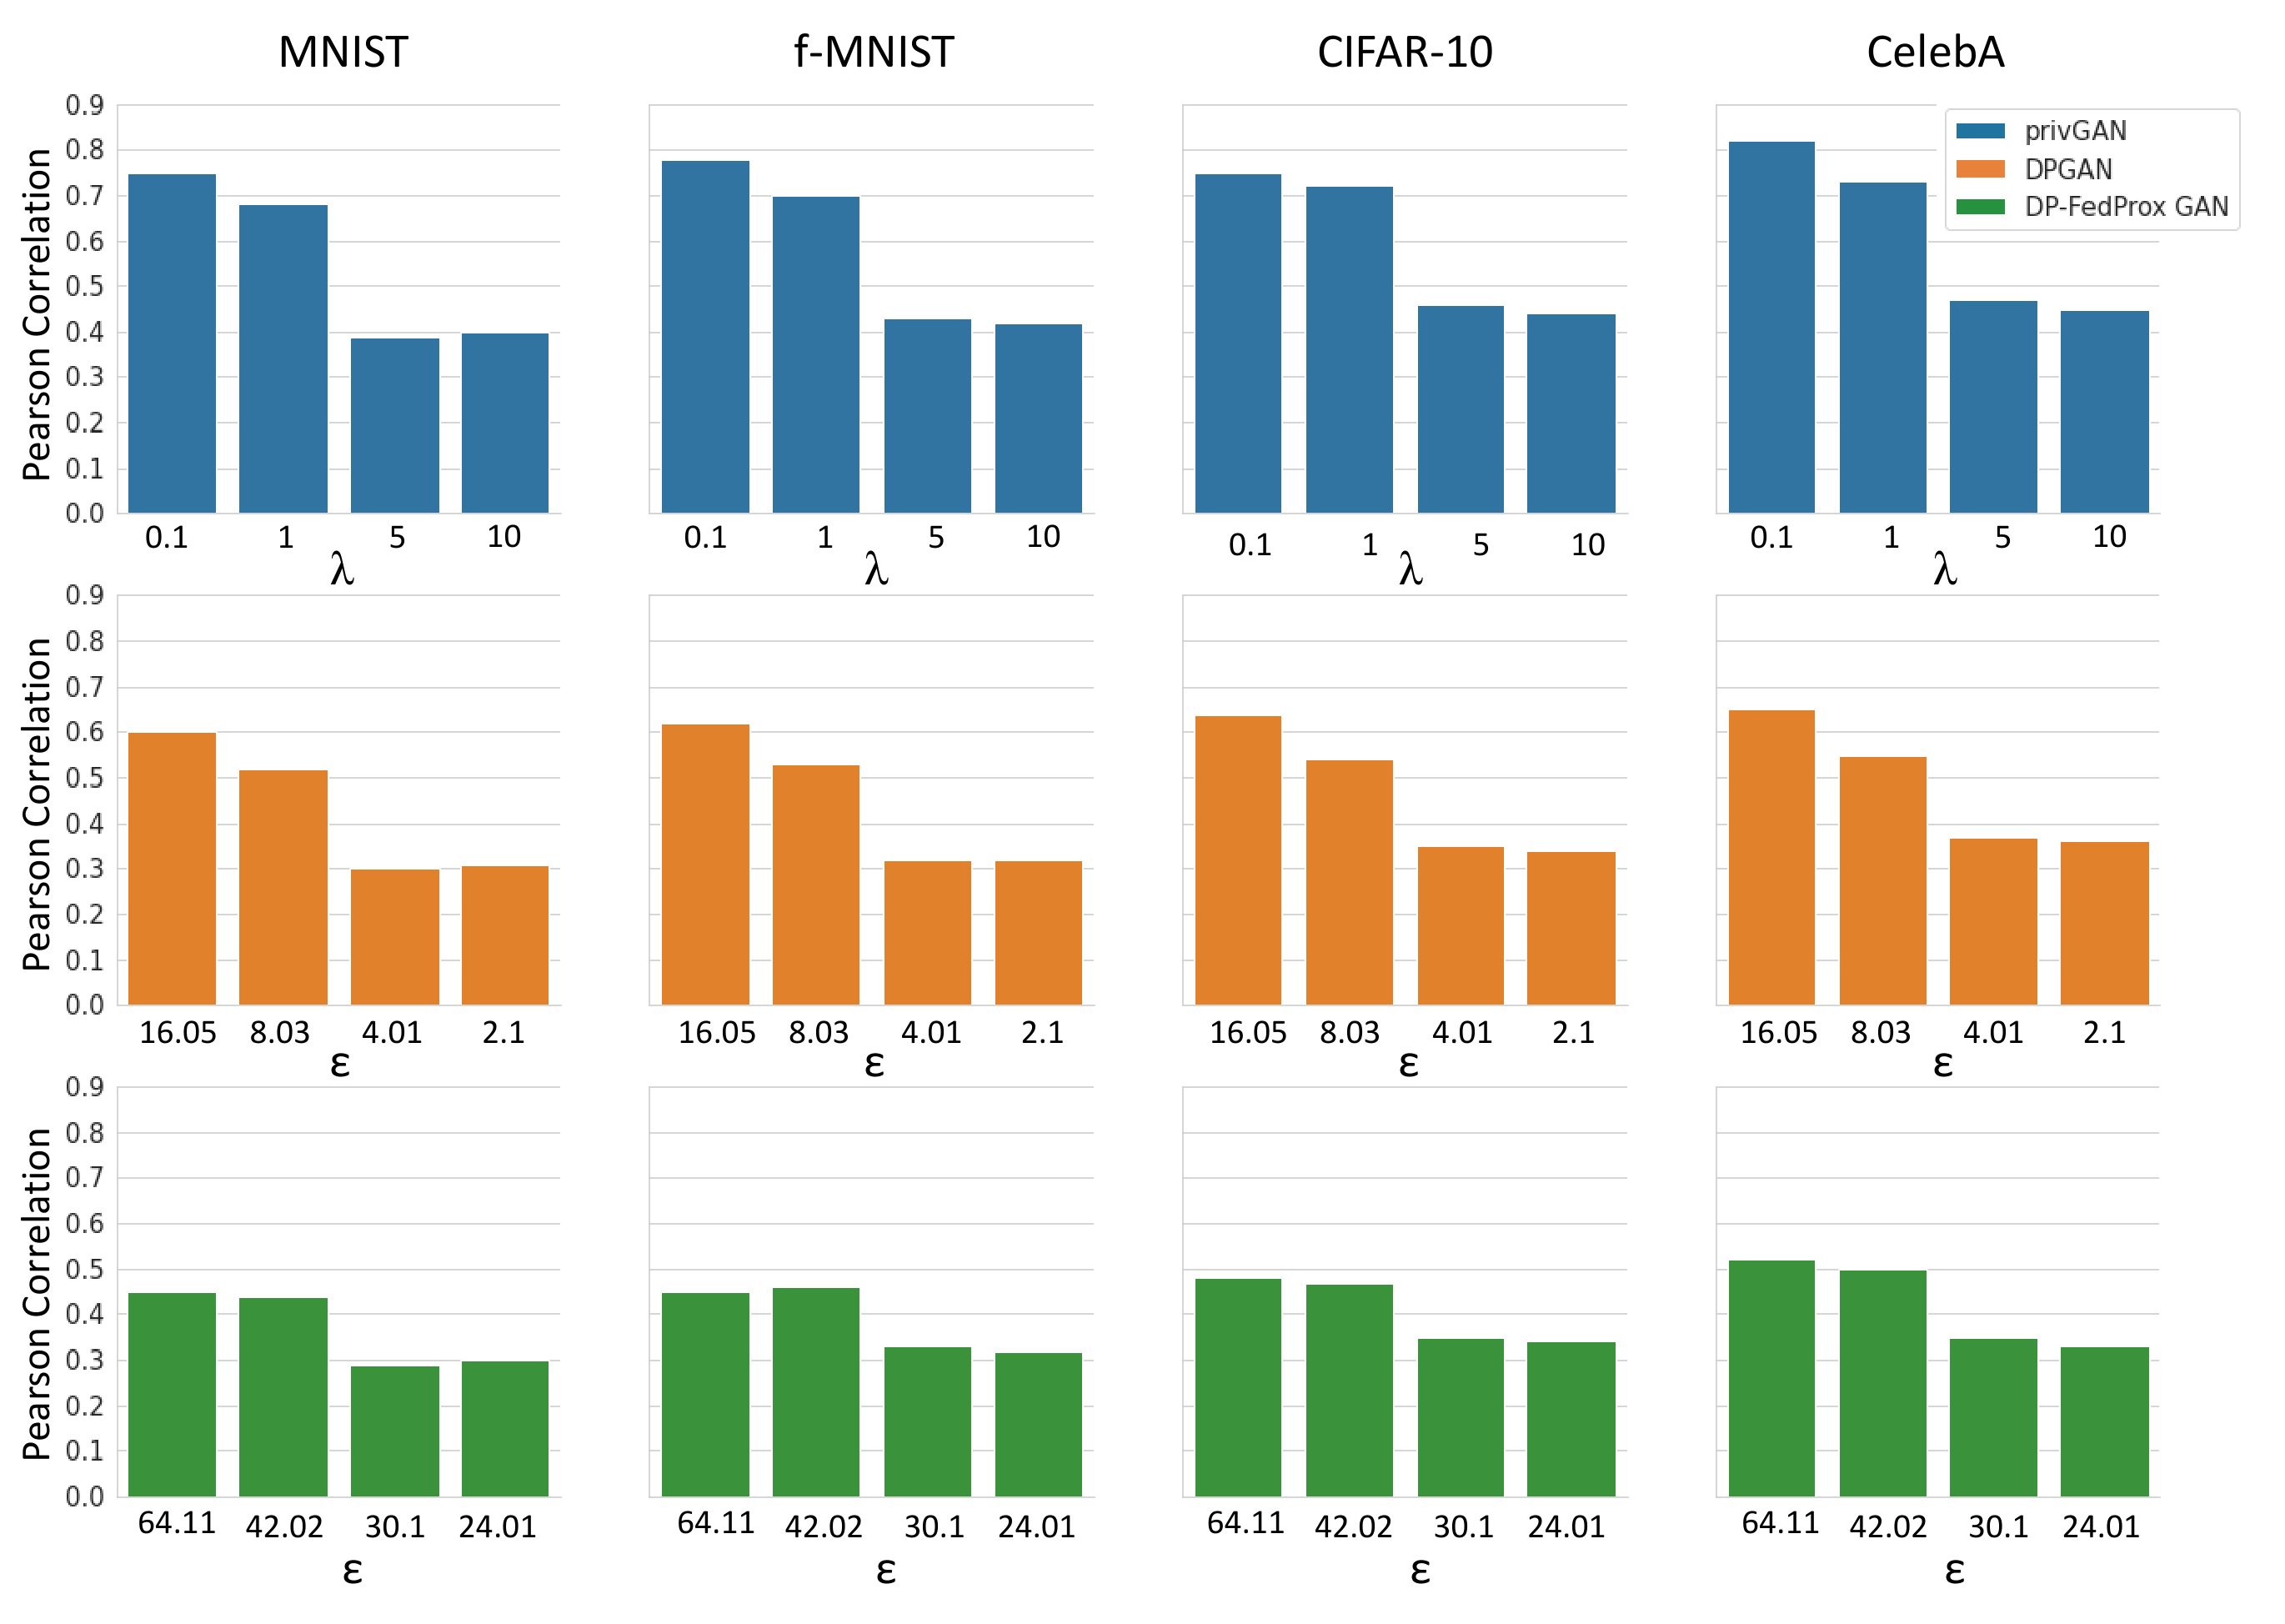
\includegraphics[width=0.8\linewidth]{Plots/IS_noise_private.png}
%  \caption{Vary Privacy Parameters in QS distribution: The Figure depicts Pearson correlation $r$ between local data size and local IS at various privacy parameters in privGAN, DPGAN, and DP-FedProx GAN. We assessed each local party's impact on overall IS for the DP-FedProx GAN by computing the difference in IS when all parties' data was used versus excluding data from a specific local party. }
%  \label{fig:IS_noise_private}
% \end{figure}





% \begin{figure}
%  \centering
%  \includegraphics[width=0.6\linewidth]{Plots/IS_local_gans_varyalpha_corr.png}
%  \caption{Vary Concentration Parameters in QS distribution: The Figure depicts Pearson correlation $r$ between local data size and local IS at various concentration parameters $\alpha$ in privGAN and DPGAN. The correlation in DP-FedProx GAN cannot be evaluated directly due to synthetic samples provided by the central server.  }
%  \label{fig:IS_local_gans_varyalpha_corr}
% \end{figure}



% \begin{figure}
%  \centering
%  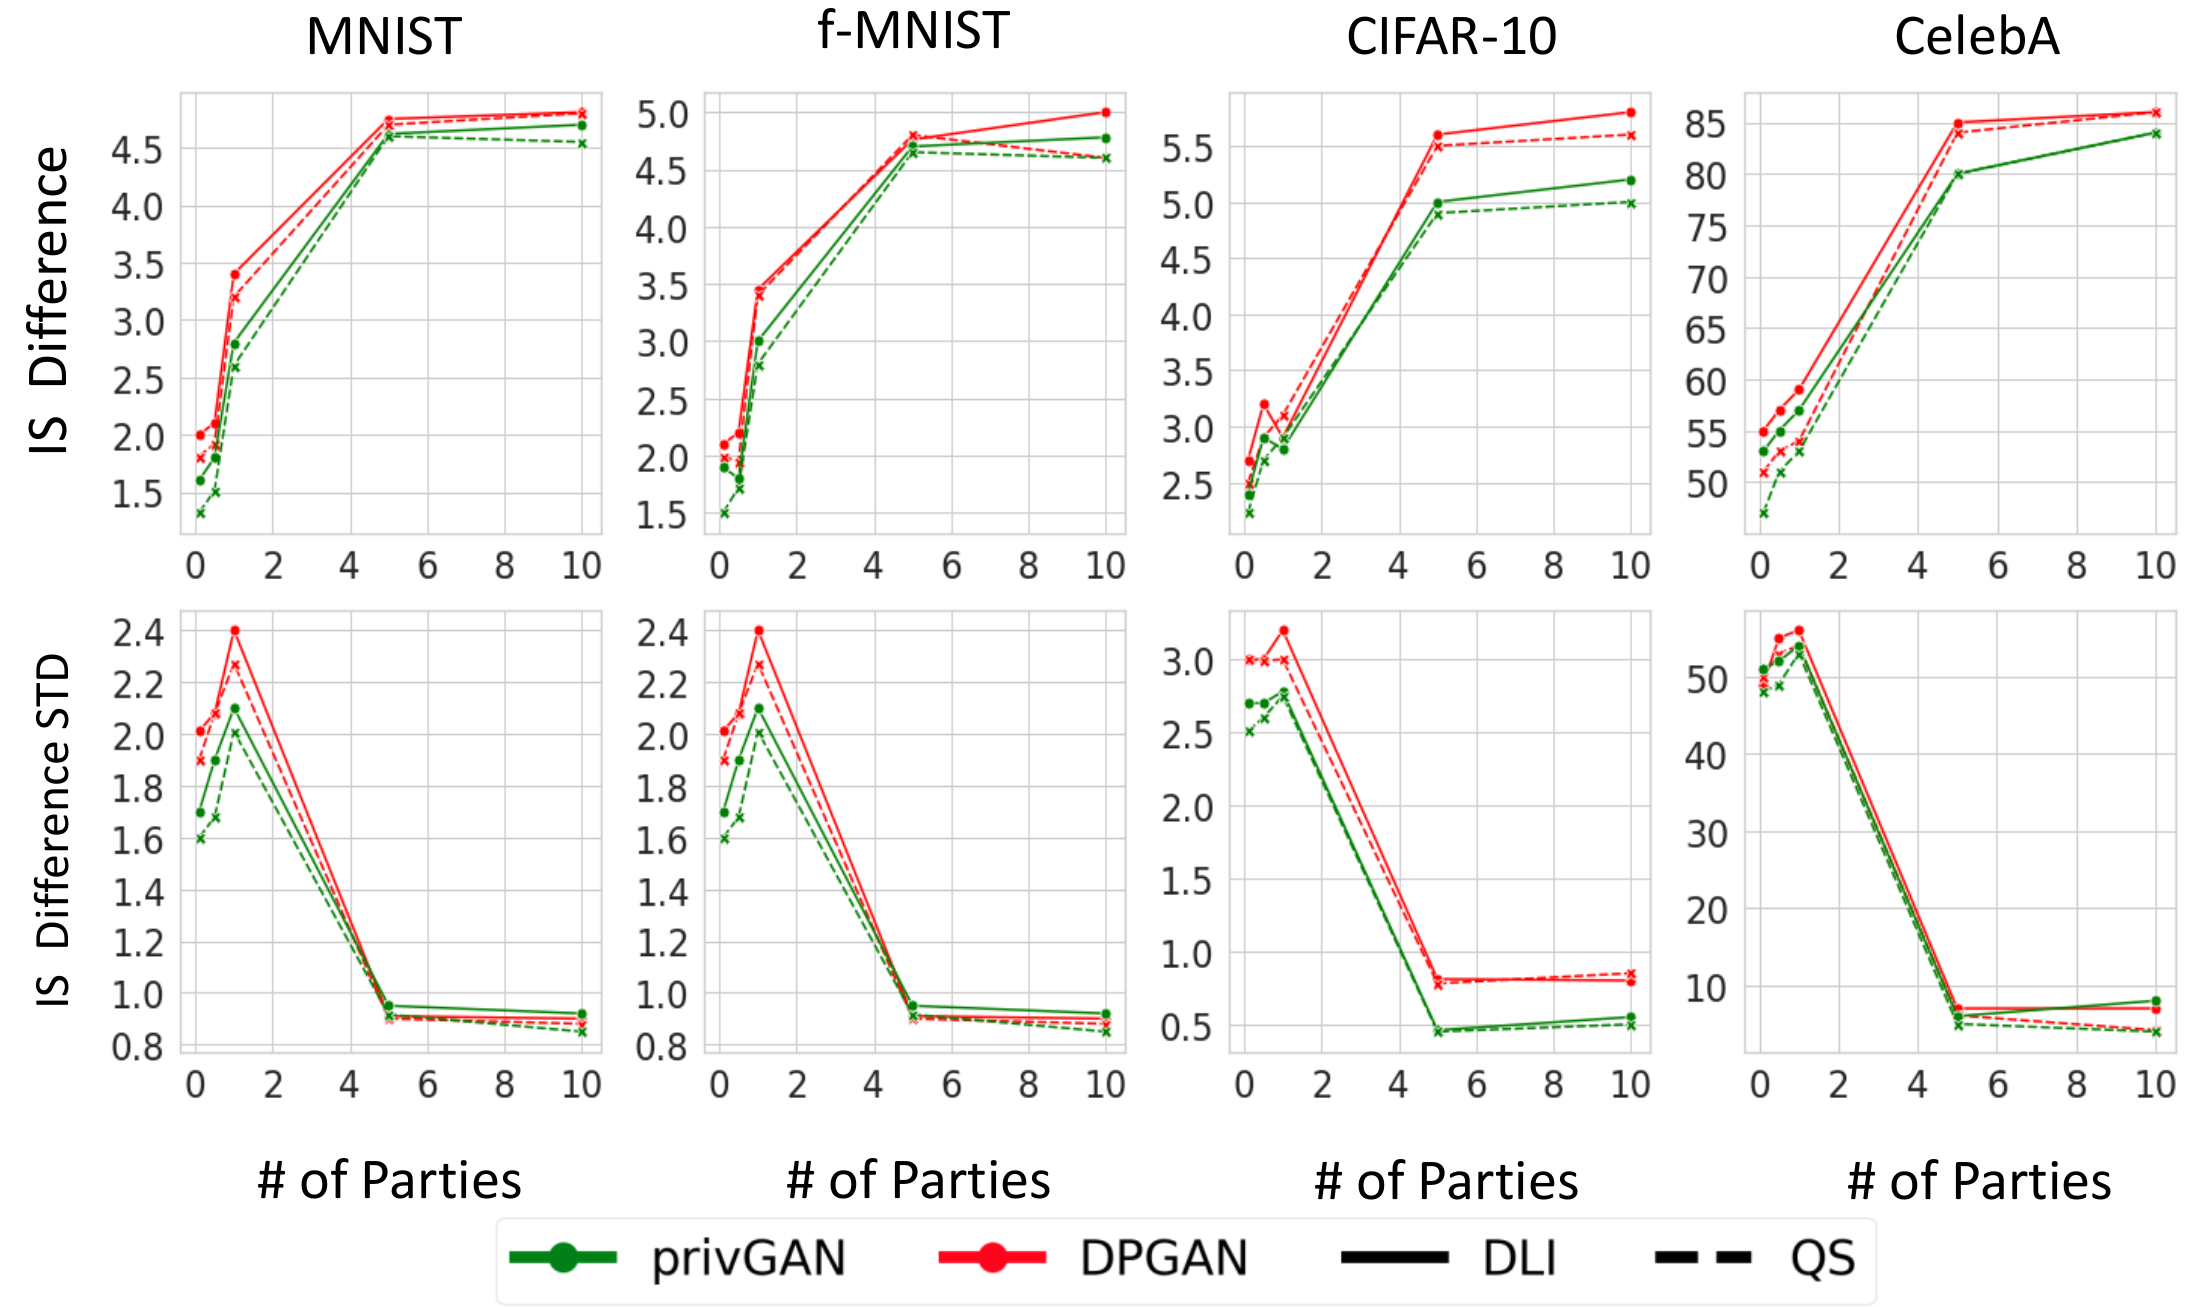
\includegraphics[width=0.8\linewidth]{Plots/IS_difference_local_gans.png}
%  \caption{Varying Concentration Parameter: The Figure depicts the average and standard deviation of IS difference between real-local-data and synthetic-local-data at various concentration parameters in privGAN and DPGAN.}
%  \label{fig:IS_difference_local_gans}
% \end{figure}


% ATTACKS






\begin{figure}
 \centering
 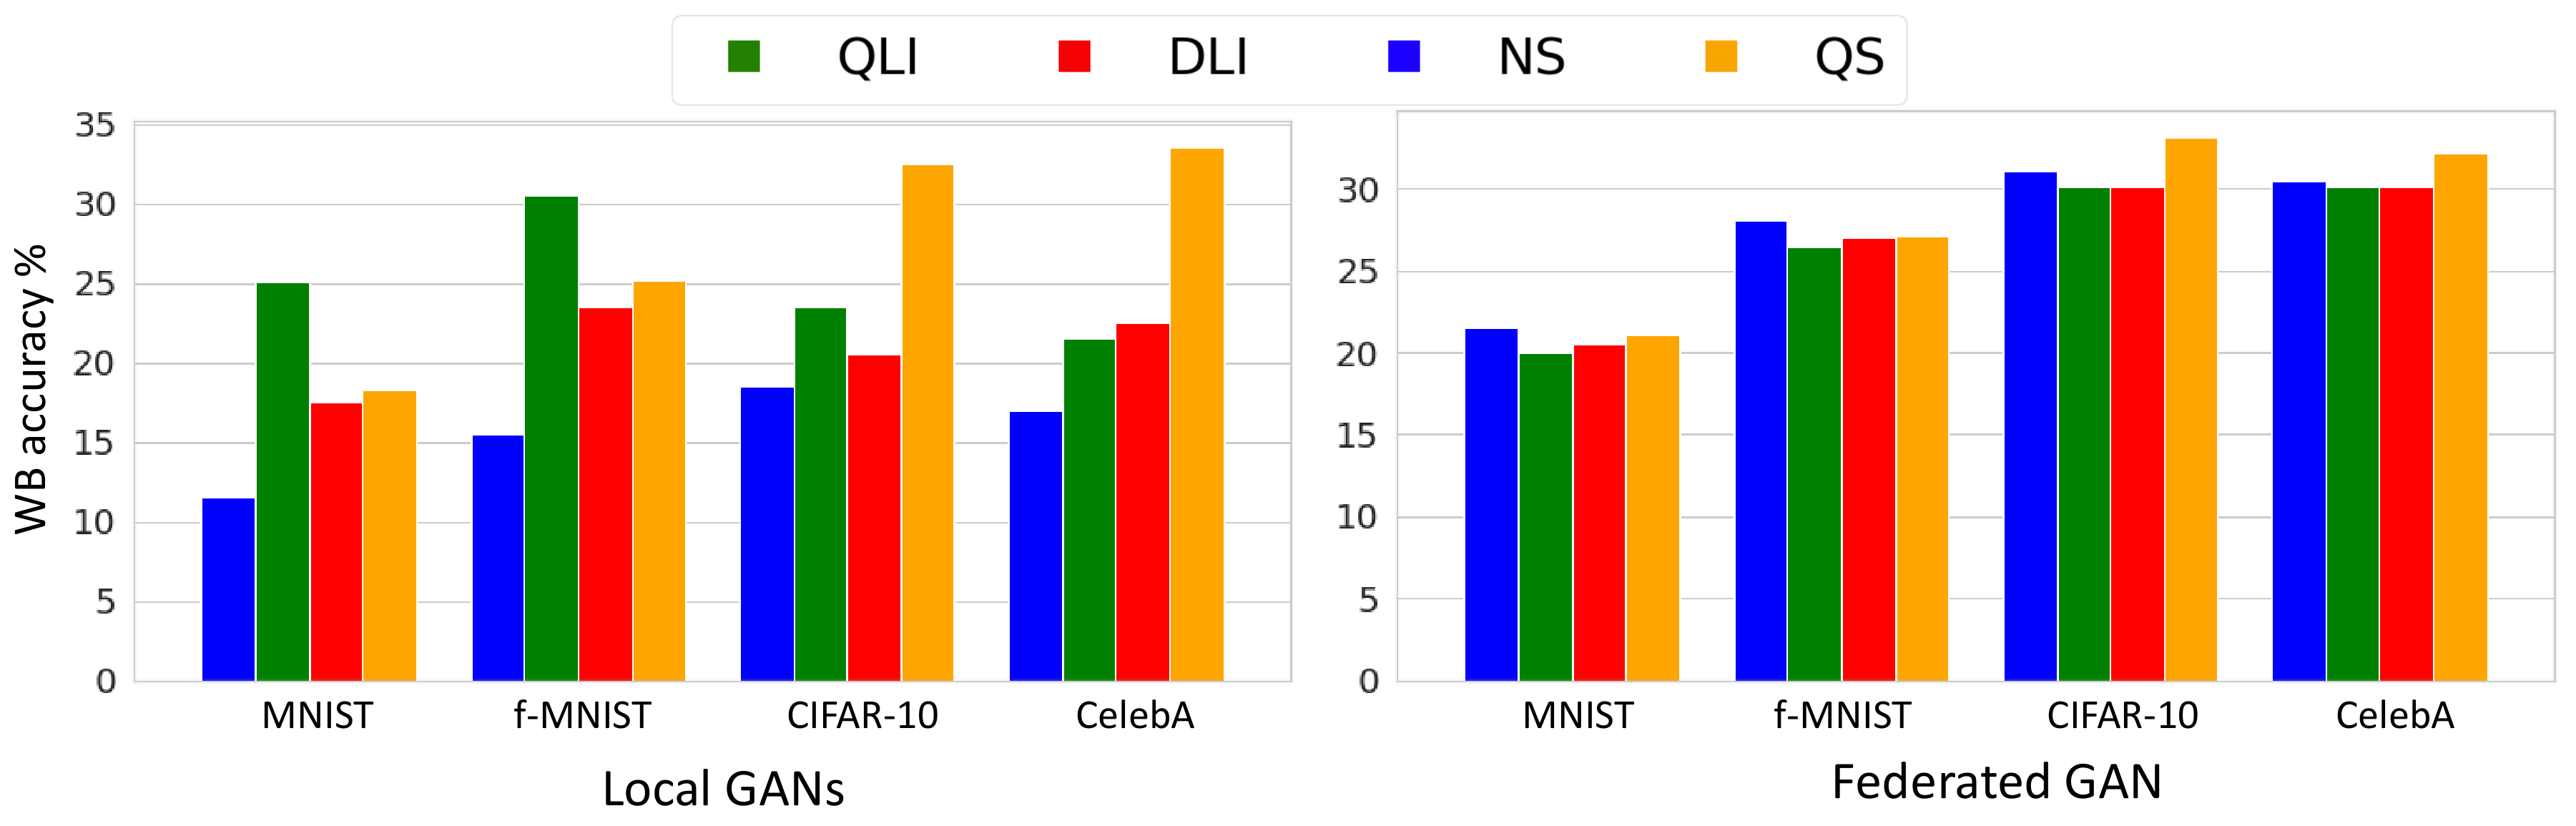
\includegraphics[width=0.7\linewidth]{Plots/baseline_WB.png}
 \caption{White-Box accuracy for Non-Private Local GANs and Federated GAN: The Figure displays the results of a white-box attack using non-private local GANs and federated GAN with $K=10$ for various distributions for each dataset.}
 \label{fig:baseline_WB}
\end{figure}


\begin{figure}
 \centering

  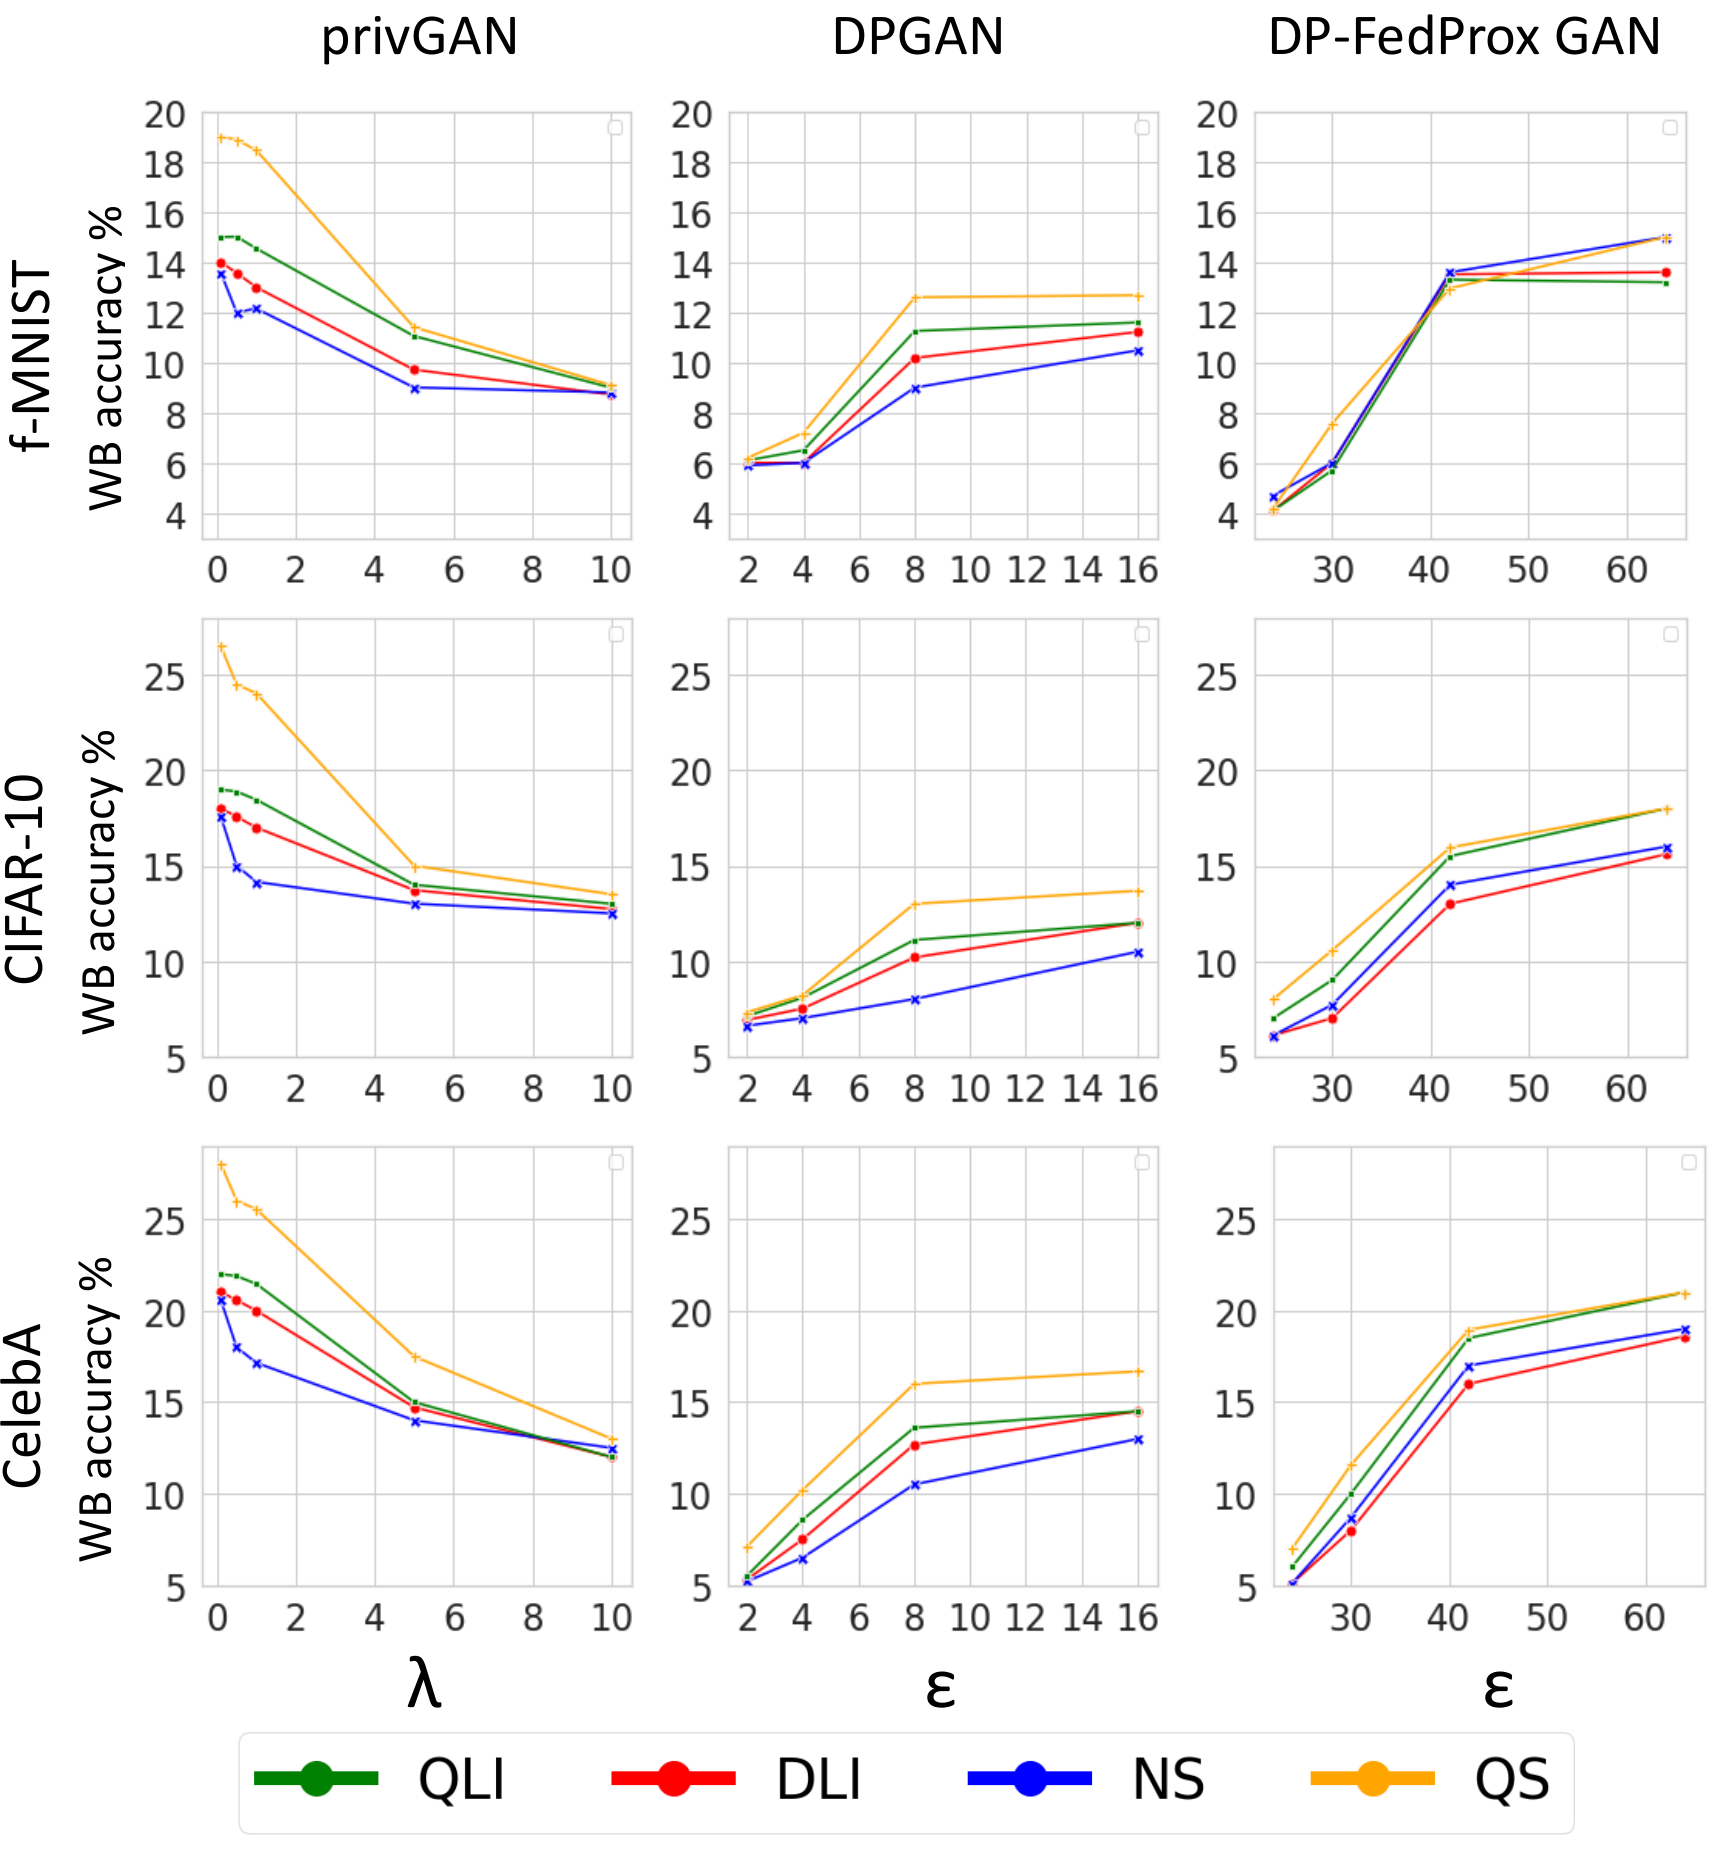
\includegraphics[width=0.6\linewidth]{Plots/vary_privacy_WB.png}

 \caption{Varying privacy parameters for White-Box Attack: The Figure shows white-box accuracy on discriminator(s) in privGAN, DPGAN, and DP-FedProx GAN for various privacy parameters.}
 \label{fig:vary_privacy_WB}
\end{figure}



\begin{figure}
 \centering
 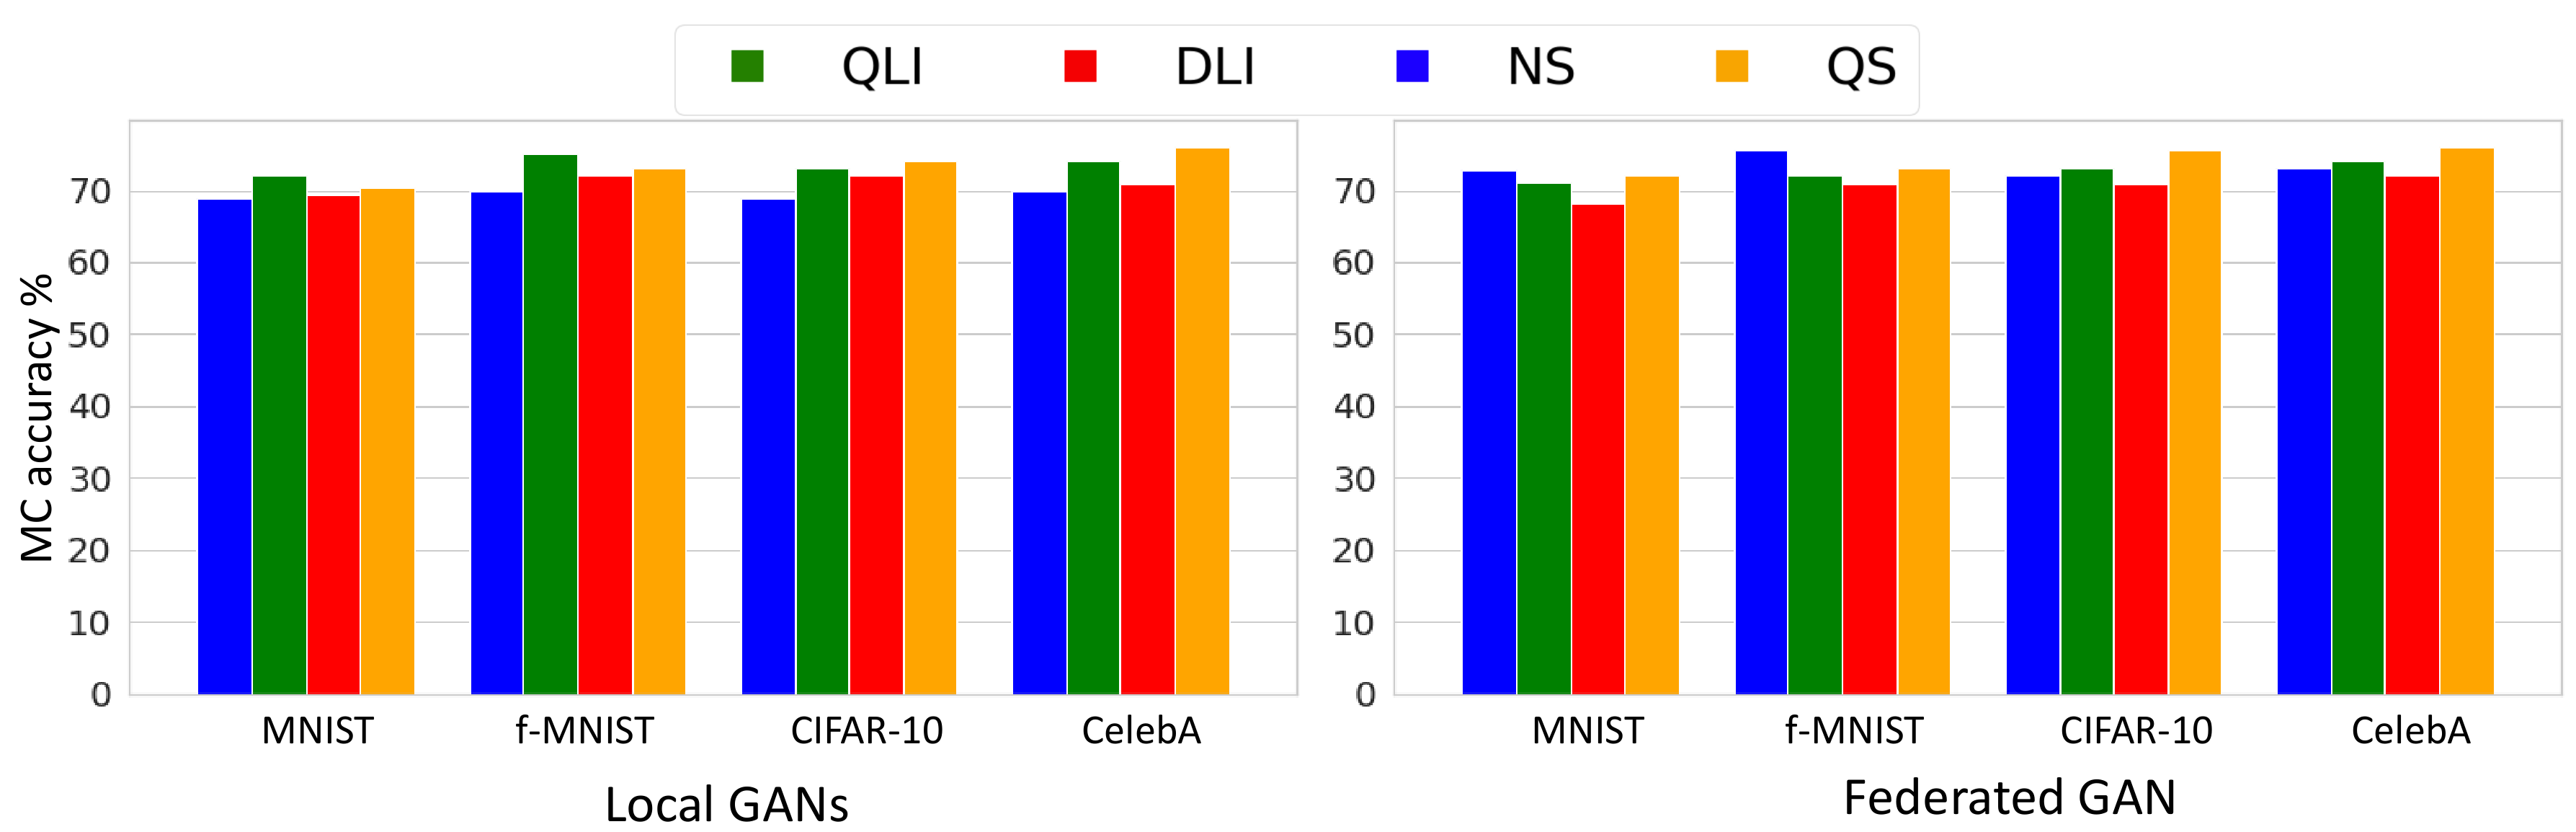
\includegraphics[width=0.7\linewidth]{Plots/MC_nonprivate.png}
 \caption{Monte-Carlo accuracy for Non-Private Local GANs and Federated GAN: The Figure displays the results of a monte-carlo attack using non-private local GANs and federated GAN with $K=10$ for various distributions for each dataset.}
 \label{fig:MC_nonprivate}
\end{figure}

\begin{figure}
 \centering
 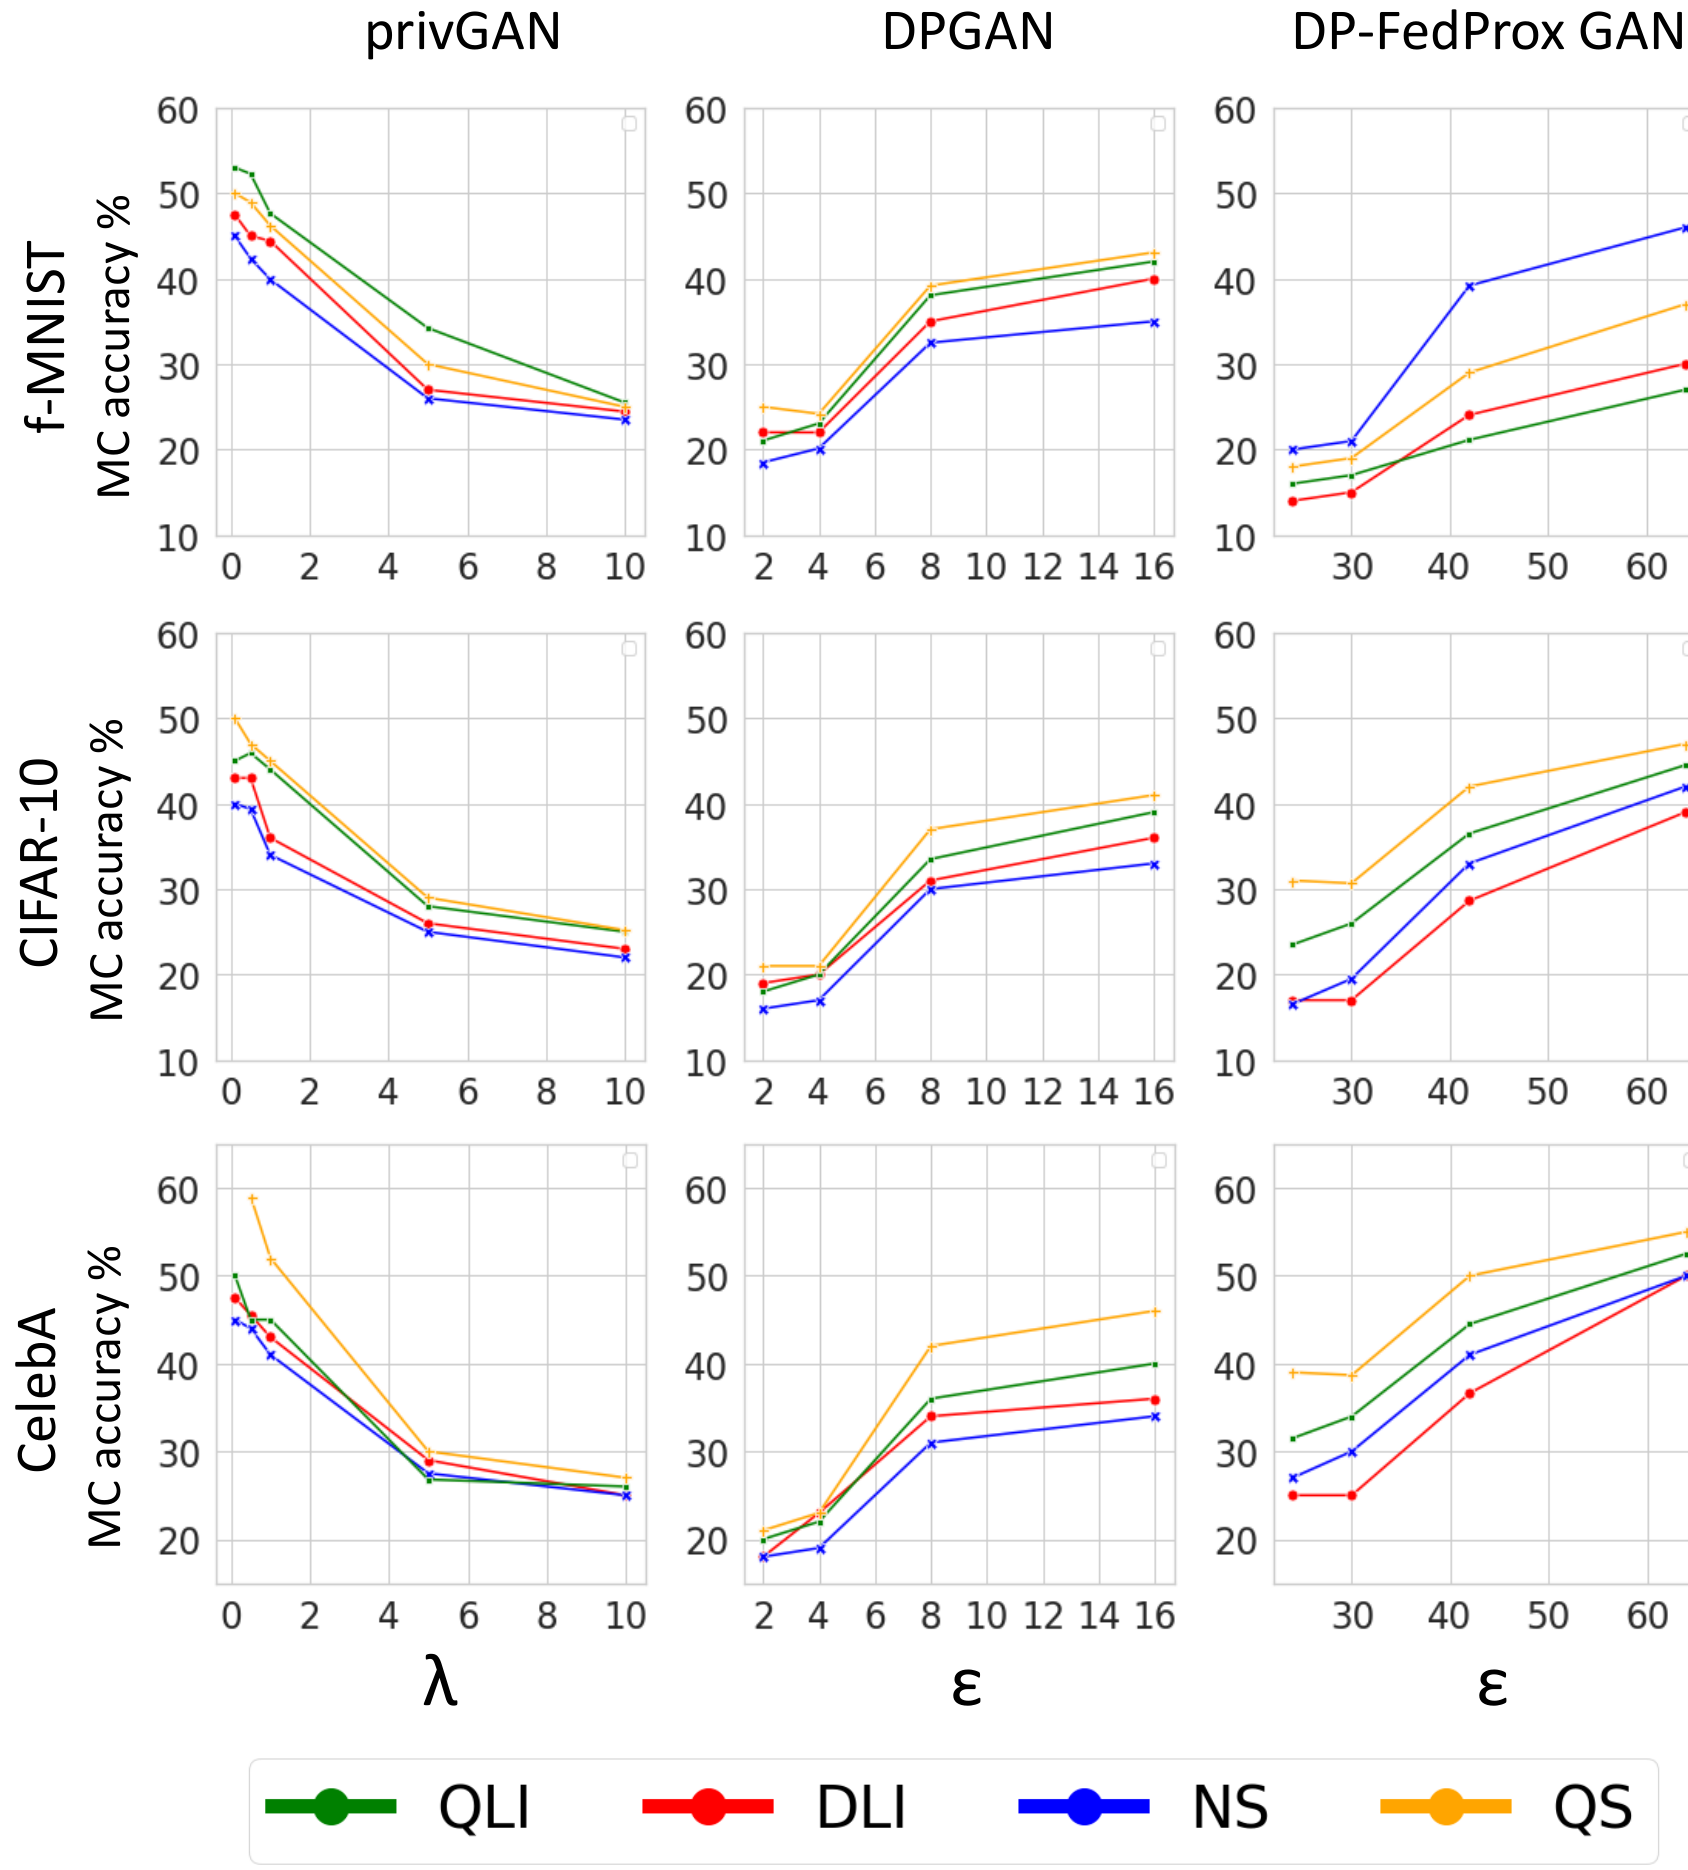
\includegraphics[width=0.6\linewidth]{Plots/vary_privacy_MC.png}
 \caption{Varying privacy parameters for Monte-Carlo Attack: The Figure shows Monte-Carlo Attack on the generator(s) in privGAN, DPGAN, and DP-FedProx GAN for various privacy parameters. }
 \label{fig:vary_privacy_MC}
\end{figure}


\begin{figure}
 \centering
 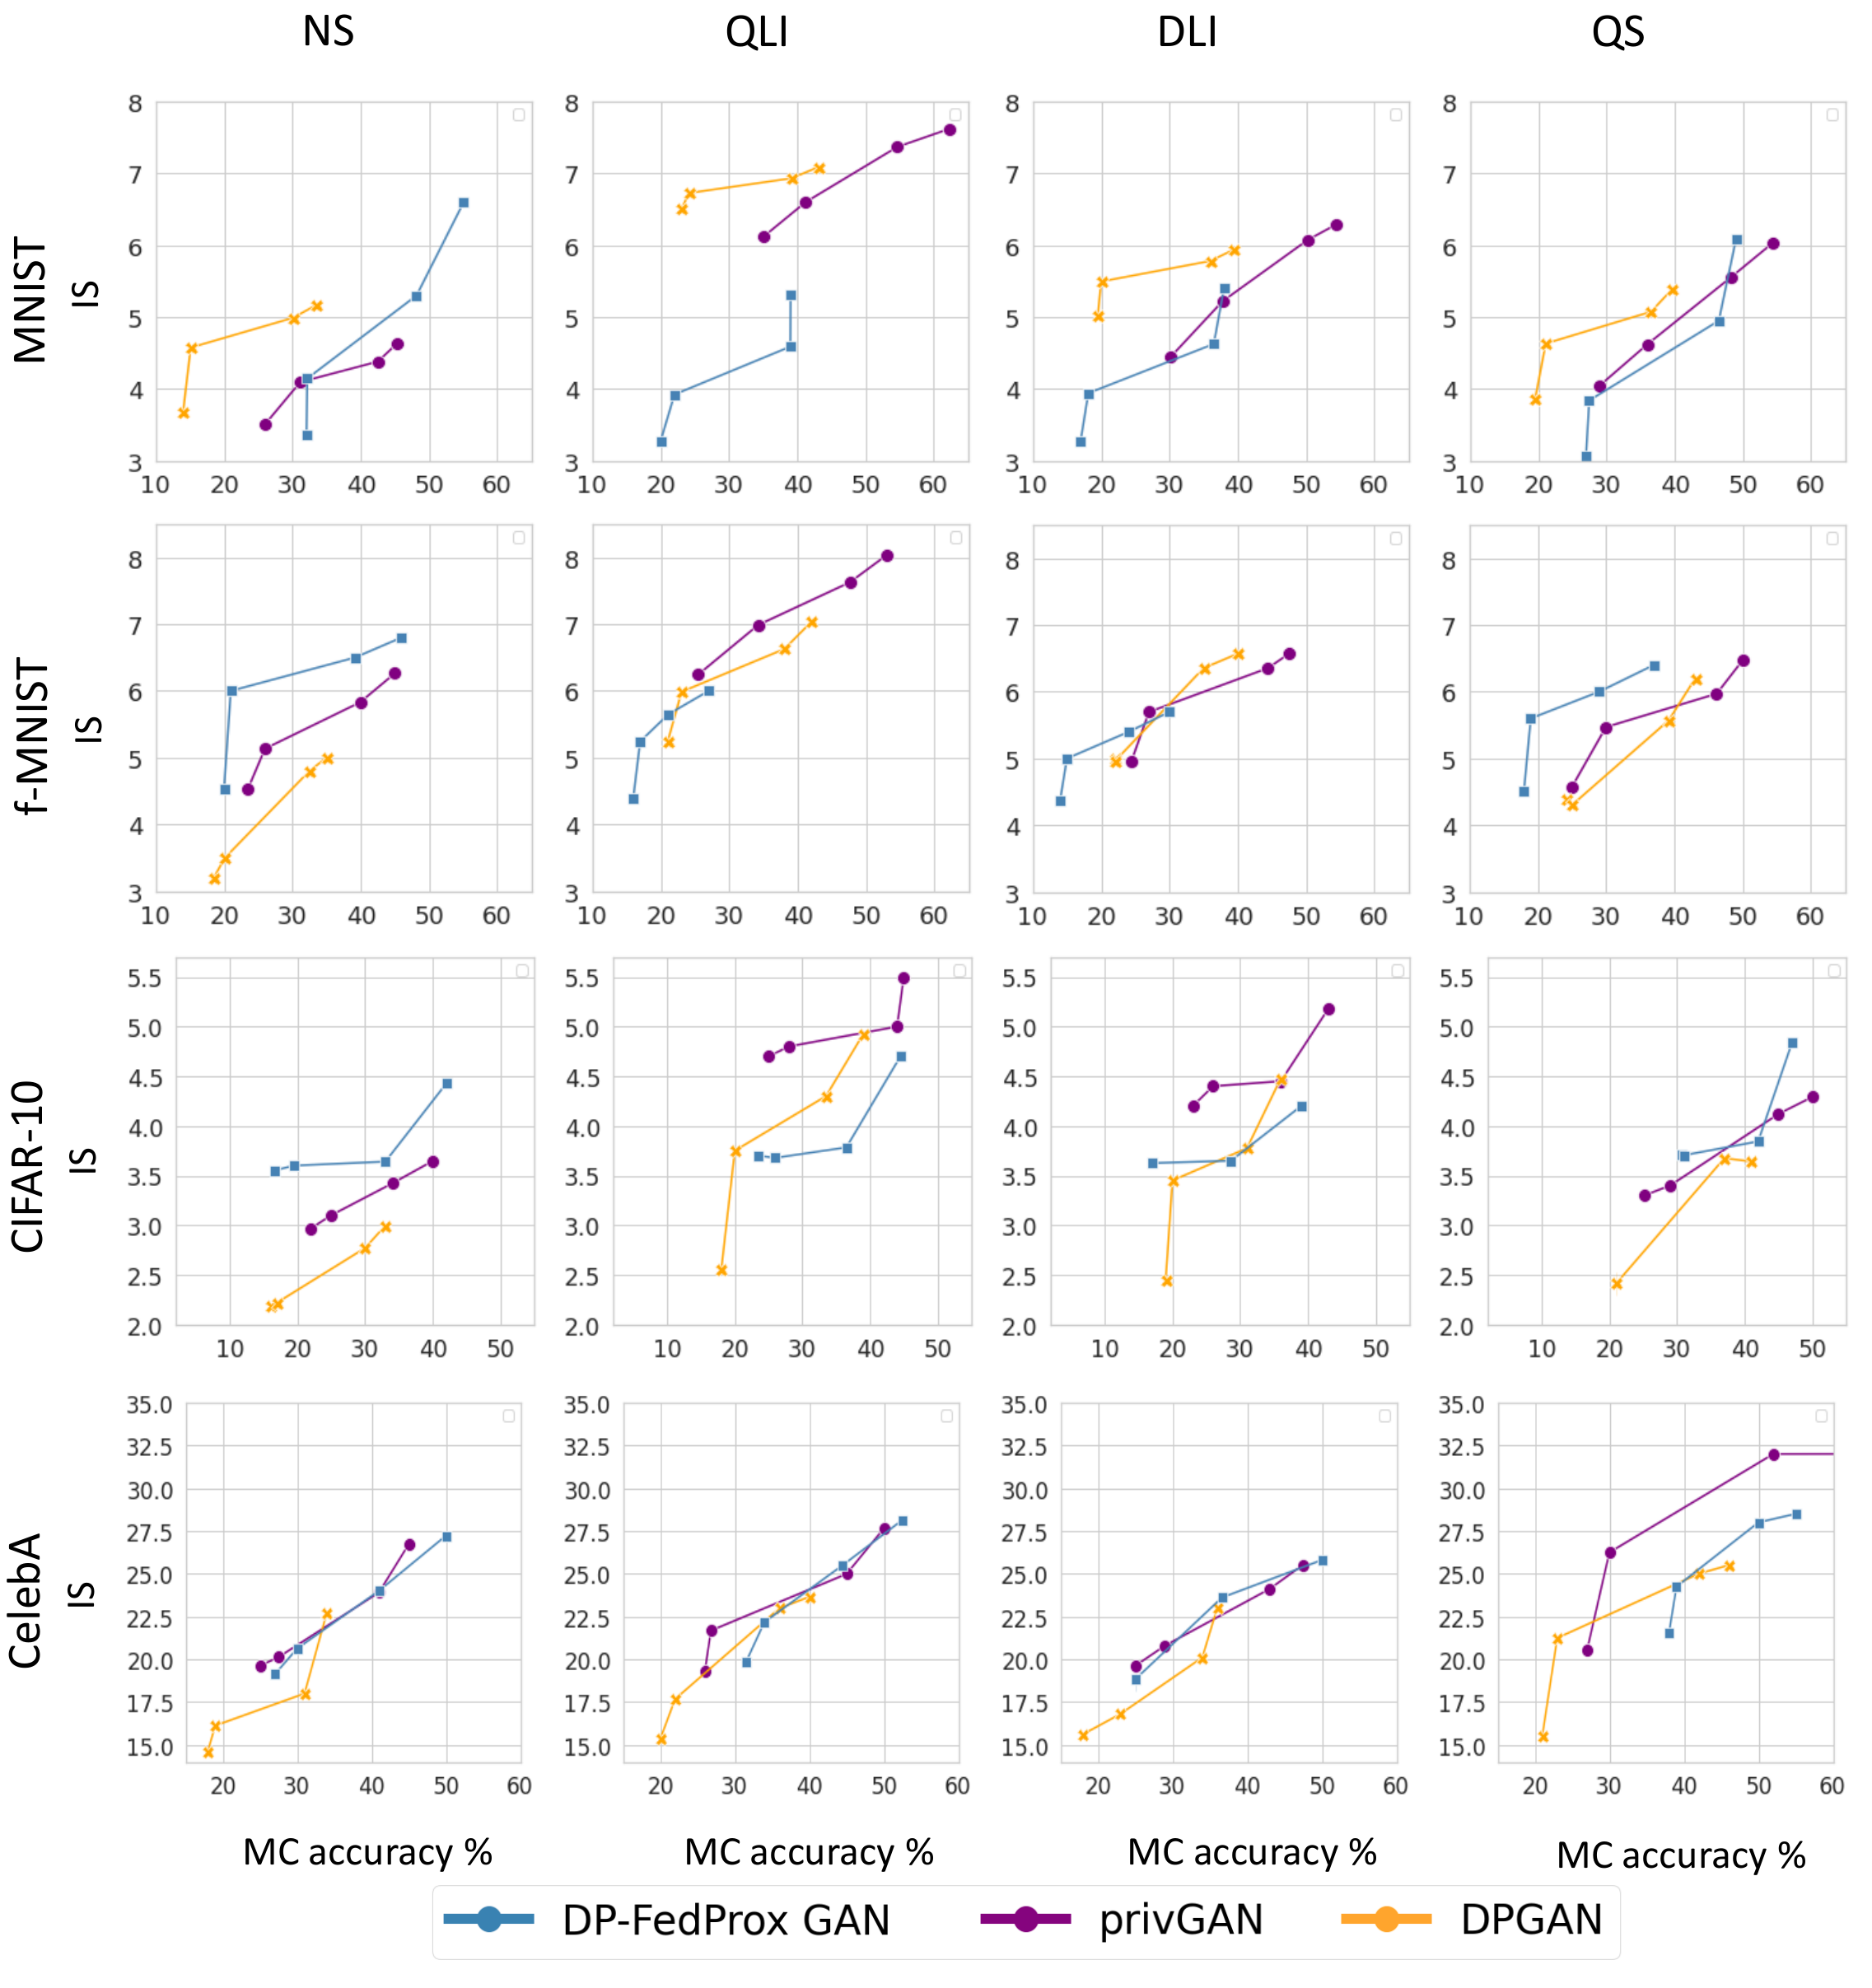
\includegraphics[width=0.8\linewidth]{Plots/varyPrivacy_MC_IS.png}
 \caption{Privacy vs. Utility: The Figure shows Monte-Carlo Attack vs Inception Score in privGAN, DPGAN, and DP-FedProx GAN for various privacy parameters.}
 \label{fig:varyPrivacy_MC_IS}
\end{figure}

\begin{figure}
 \centering
 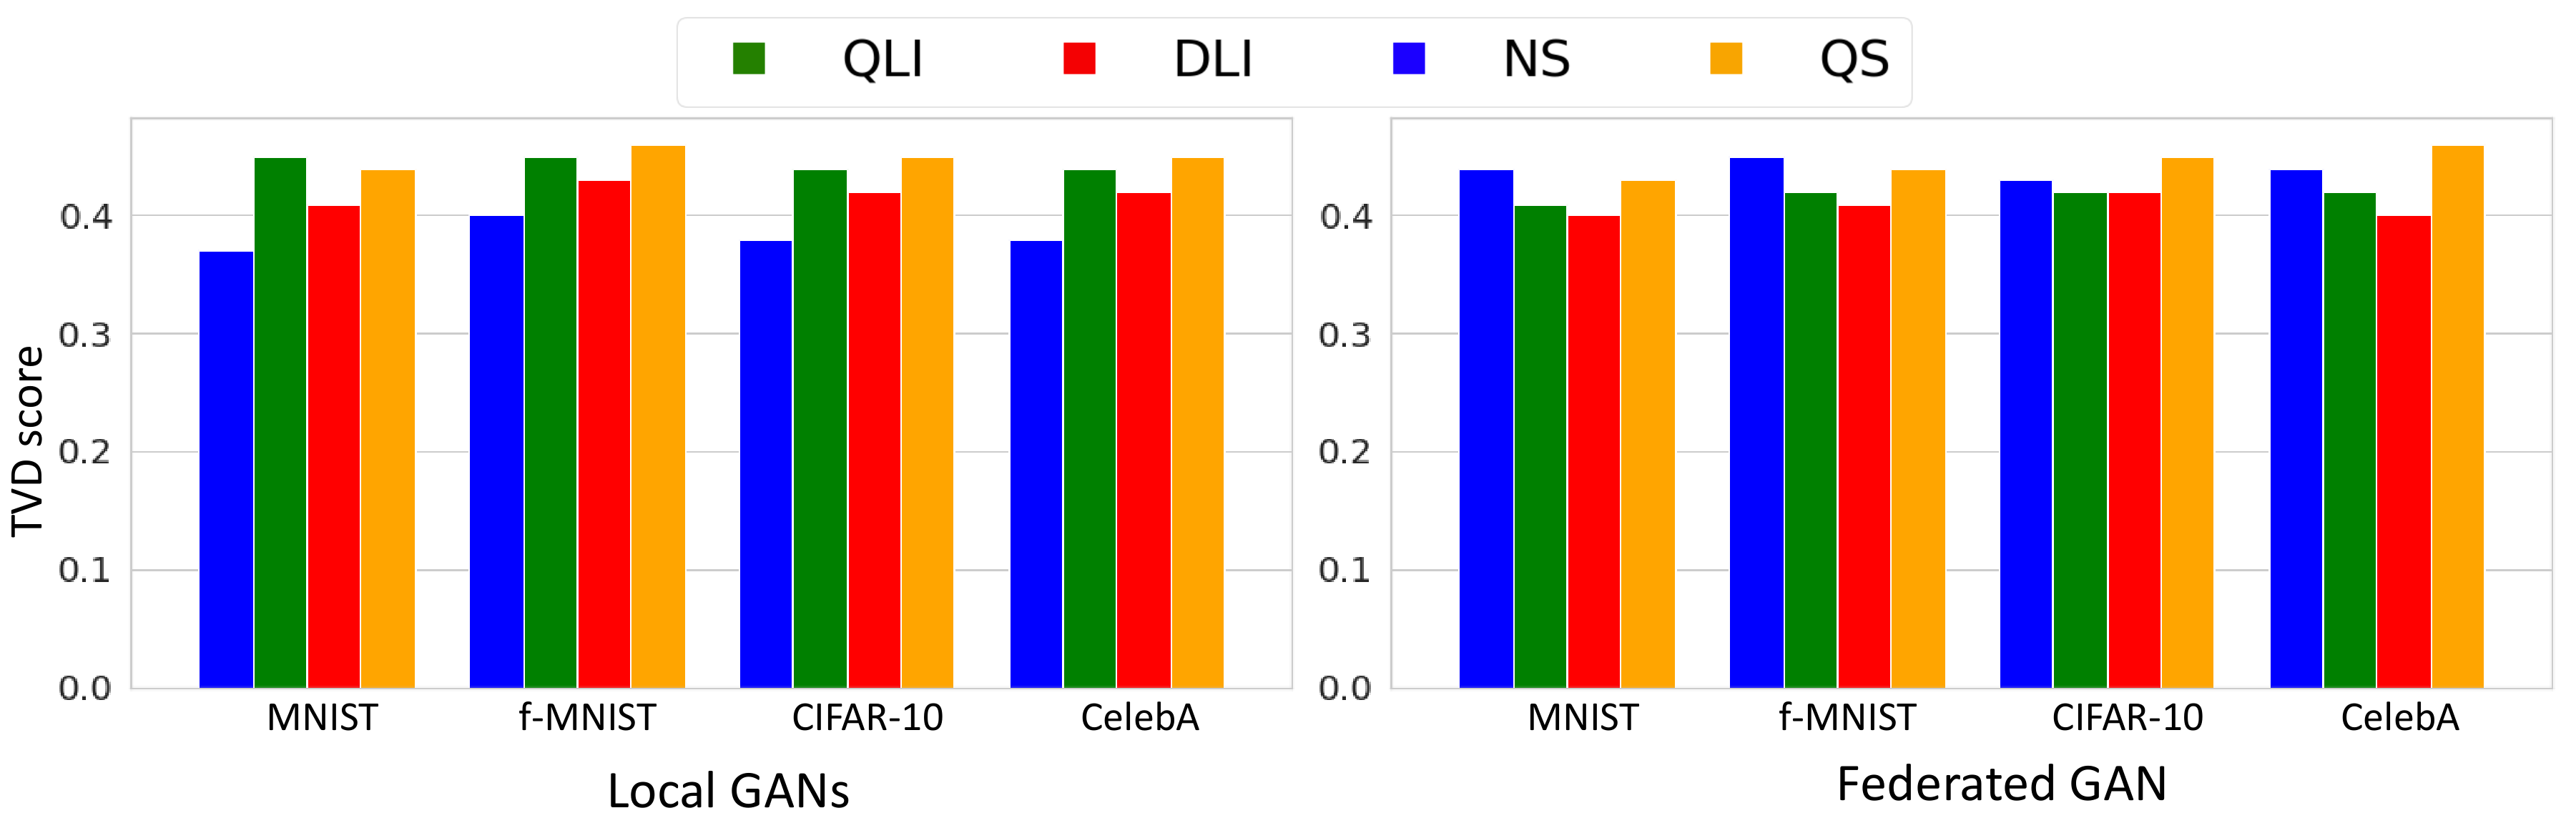
\includegraphics[width=0.7\linewidth]{Plots/TVD_nonprivate.png}
 \caption{TVD score for Non-Private Local GANs and Federated GAN: The Figure displays the results of a TVD attack score using non-private local GANs and federated GAN with $K=10$ for various distributions for each dataset.}
 \label{fig:TVD_nonprivate}
\end{figure}


\begin{figure}
 \centering
 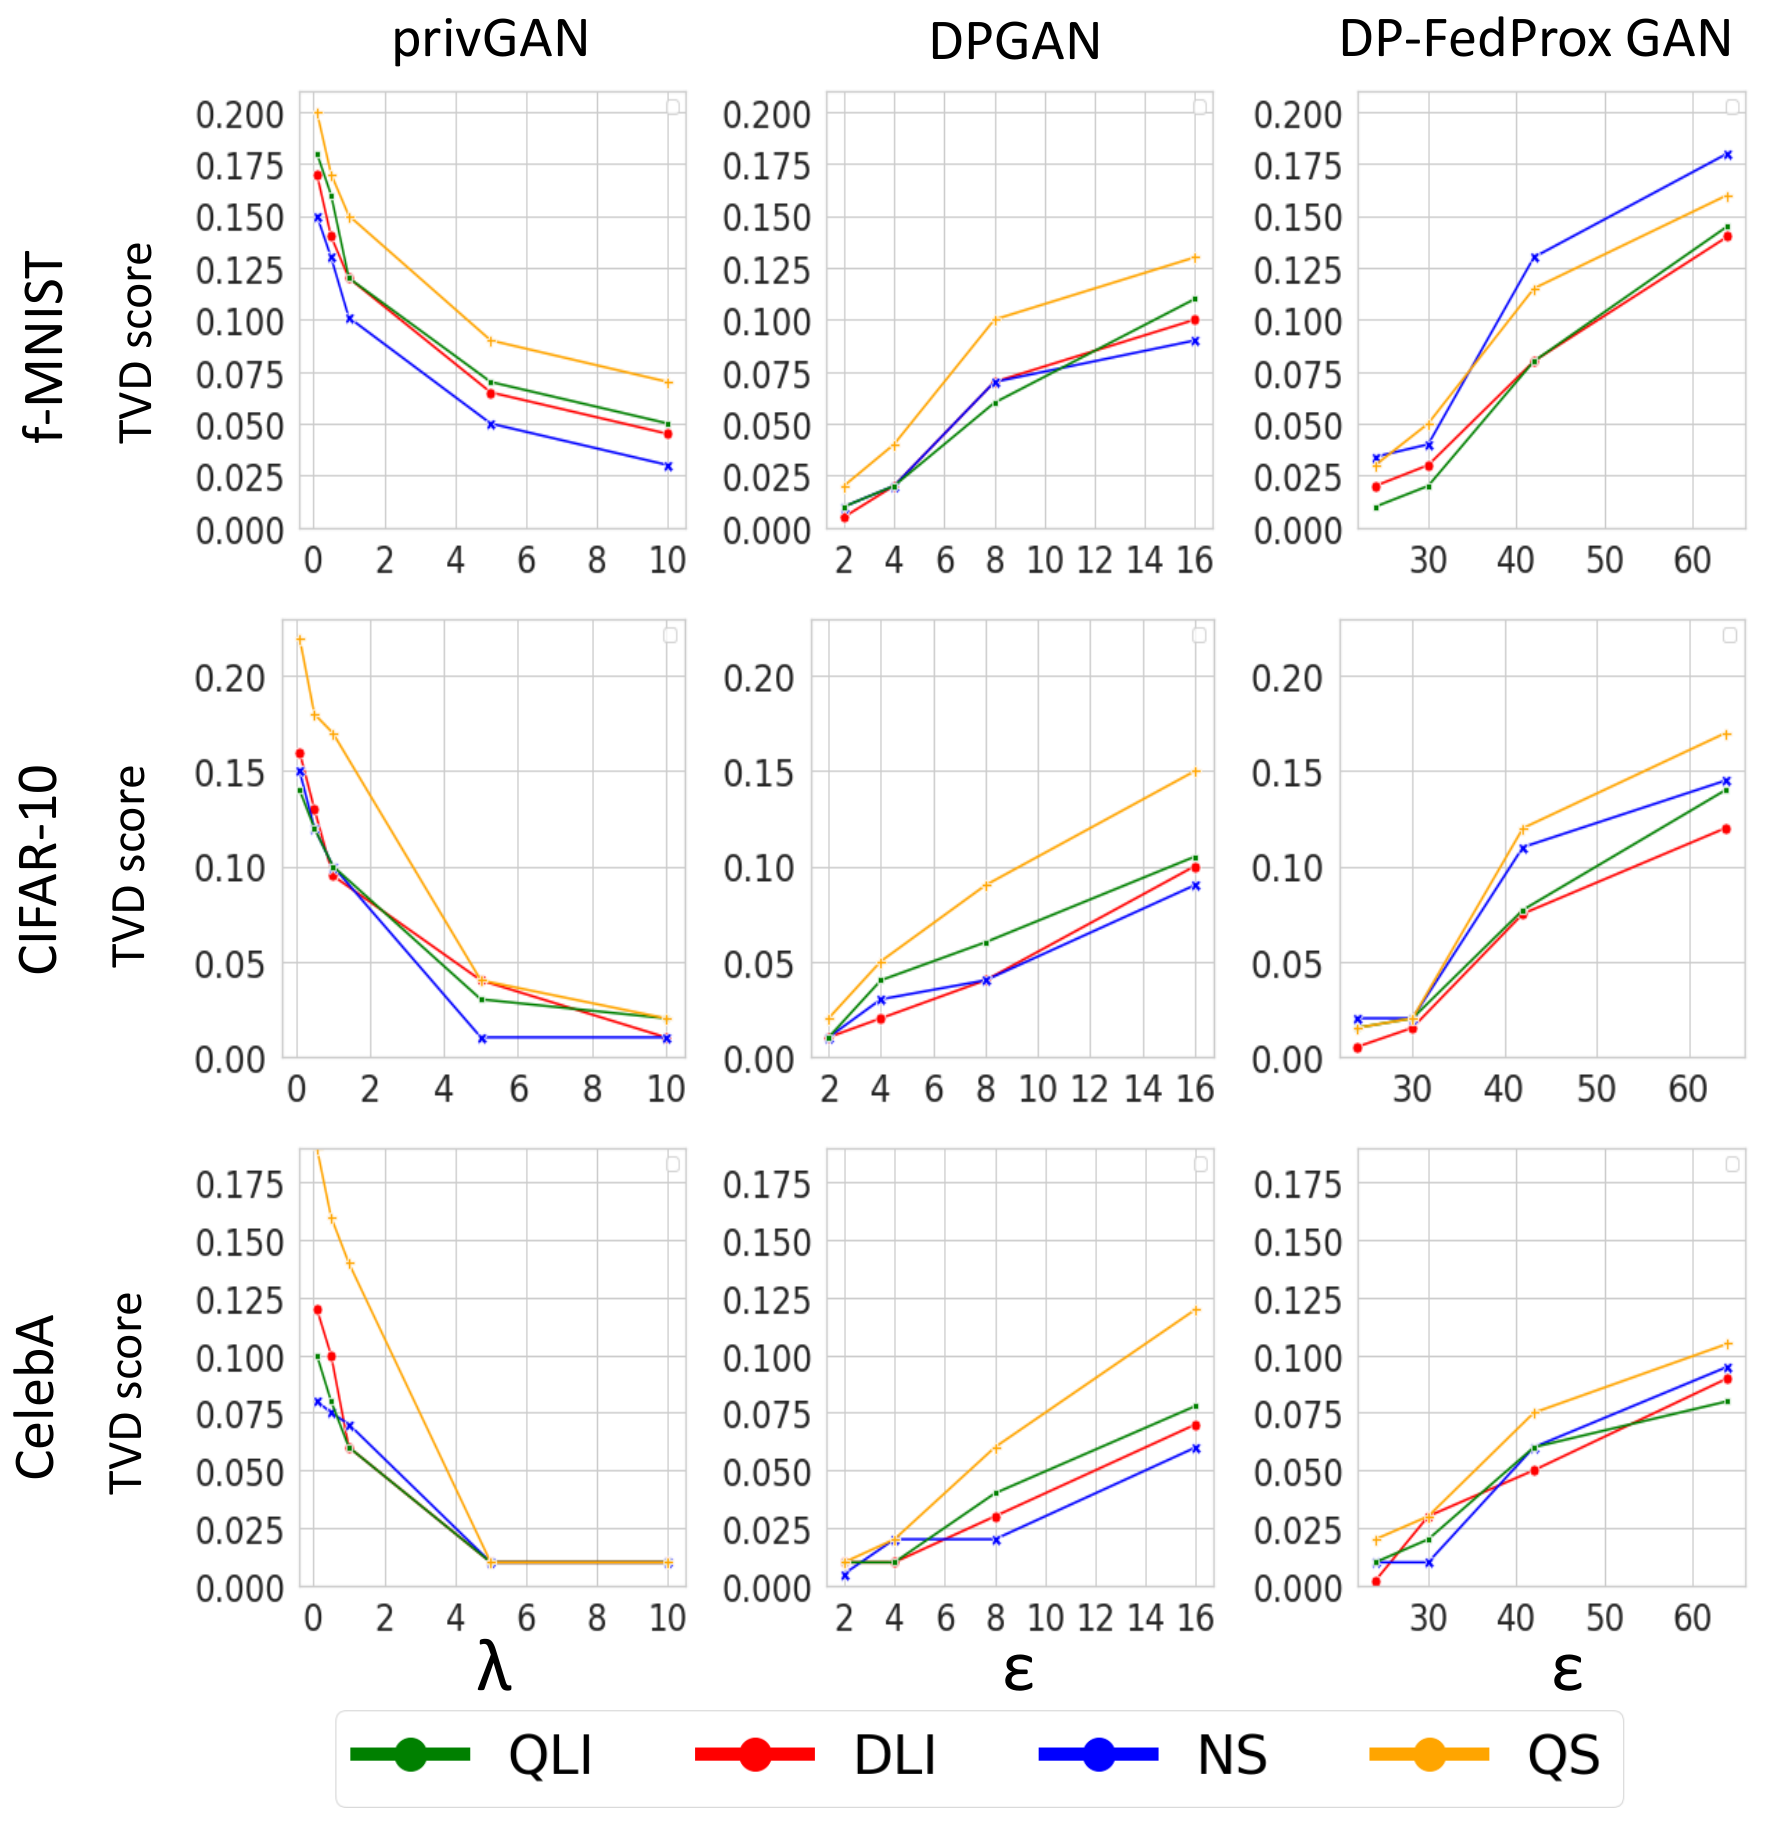
\includegraphics[width=0.6\linewidth]{Plots/vary_privacy_TVD.png}
 \caption{Varying privacy parameters for TVD Attack: For different privacy parameters, the Figure displays the TVD attack score on the discriminator(s) in privGAN, DPGAN, and DP-FedProx GAN.}
 \label{fig:vary_privacy_TVD}
\end{figure}



\begin{figure}
 \centering
 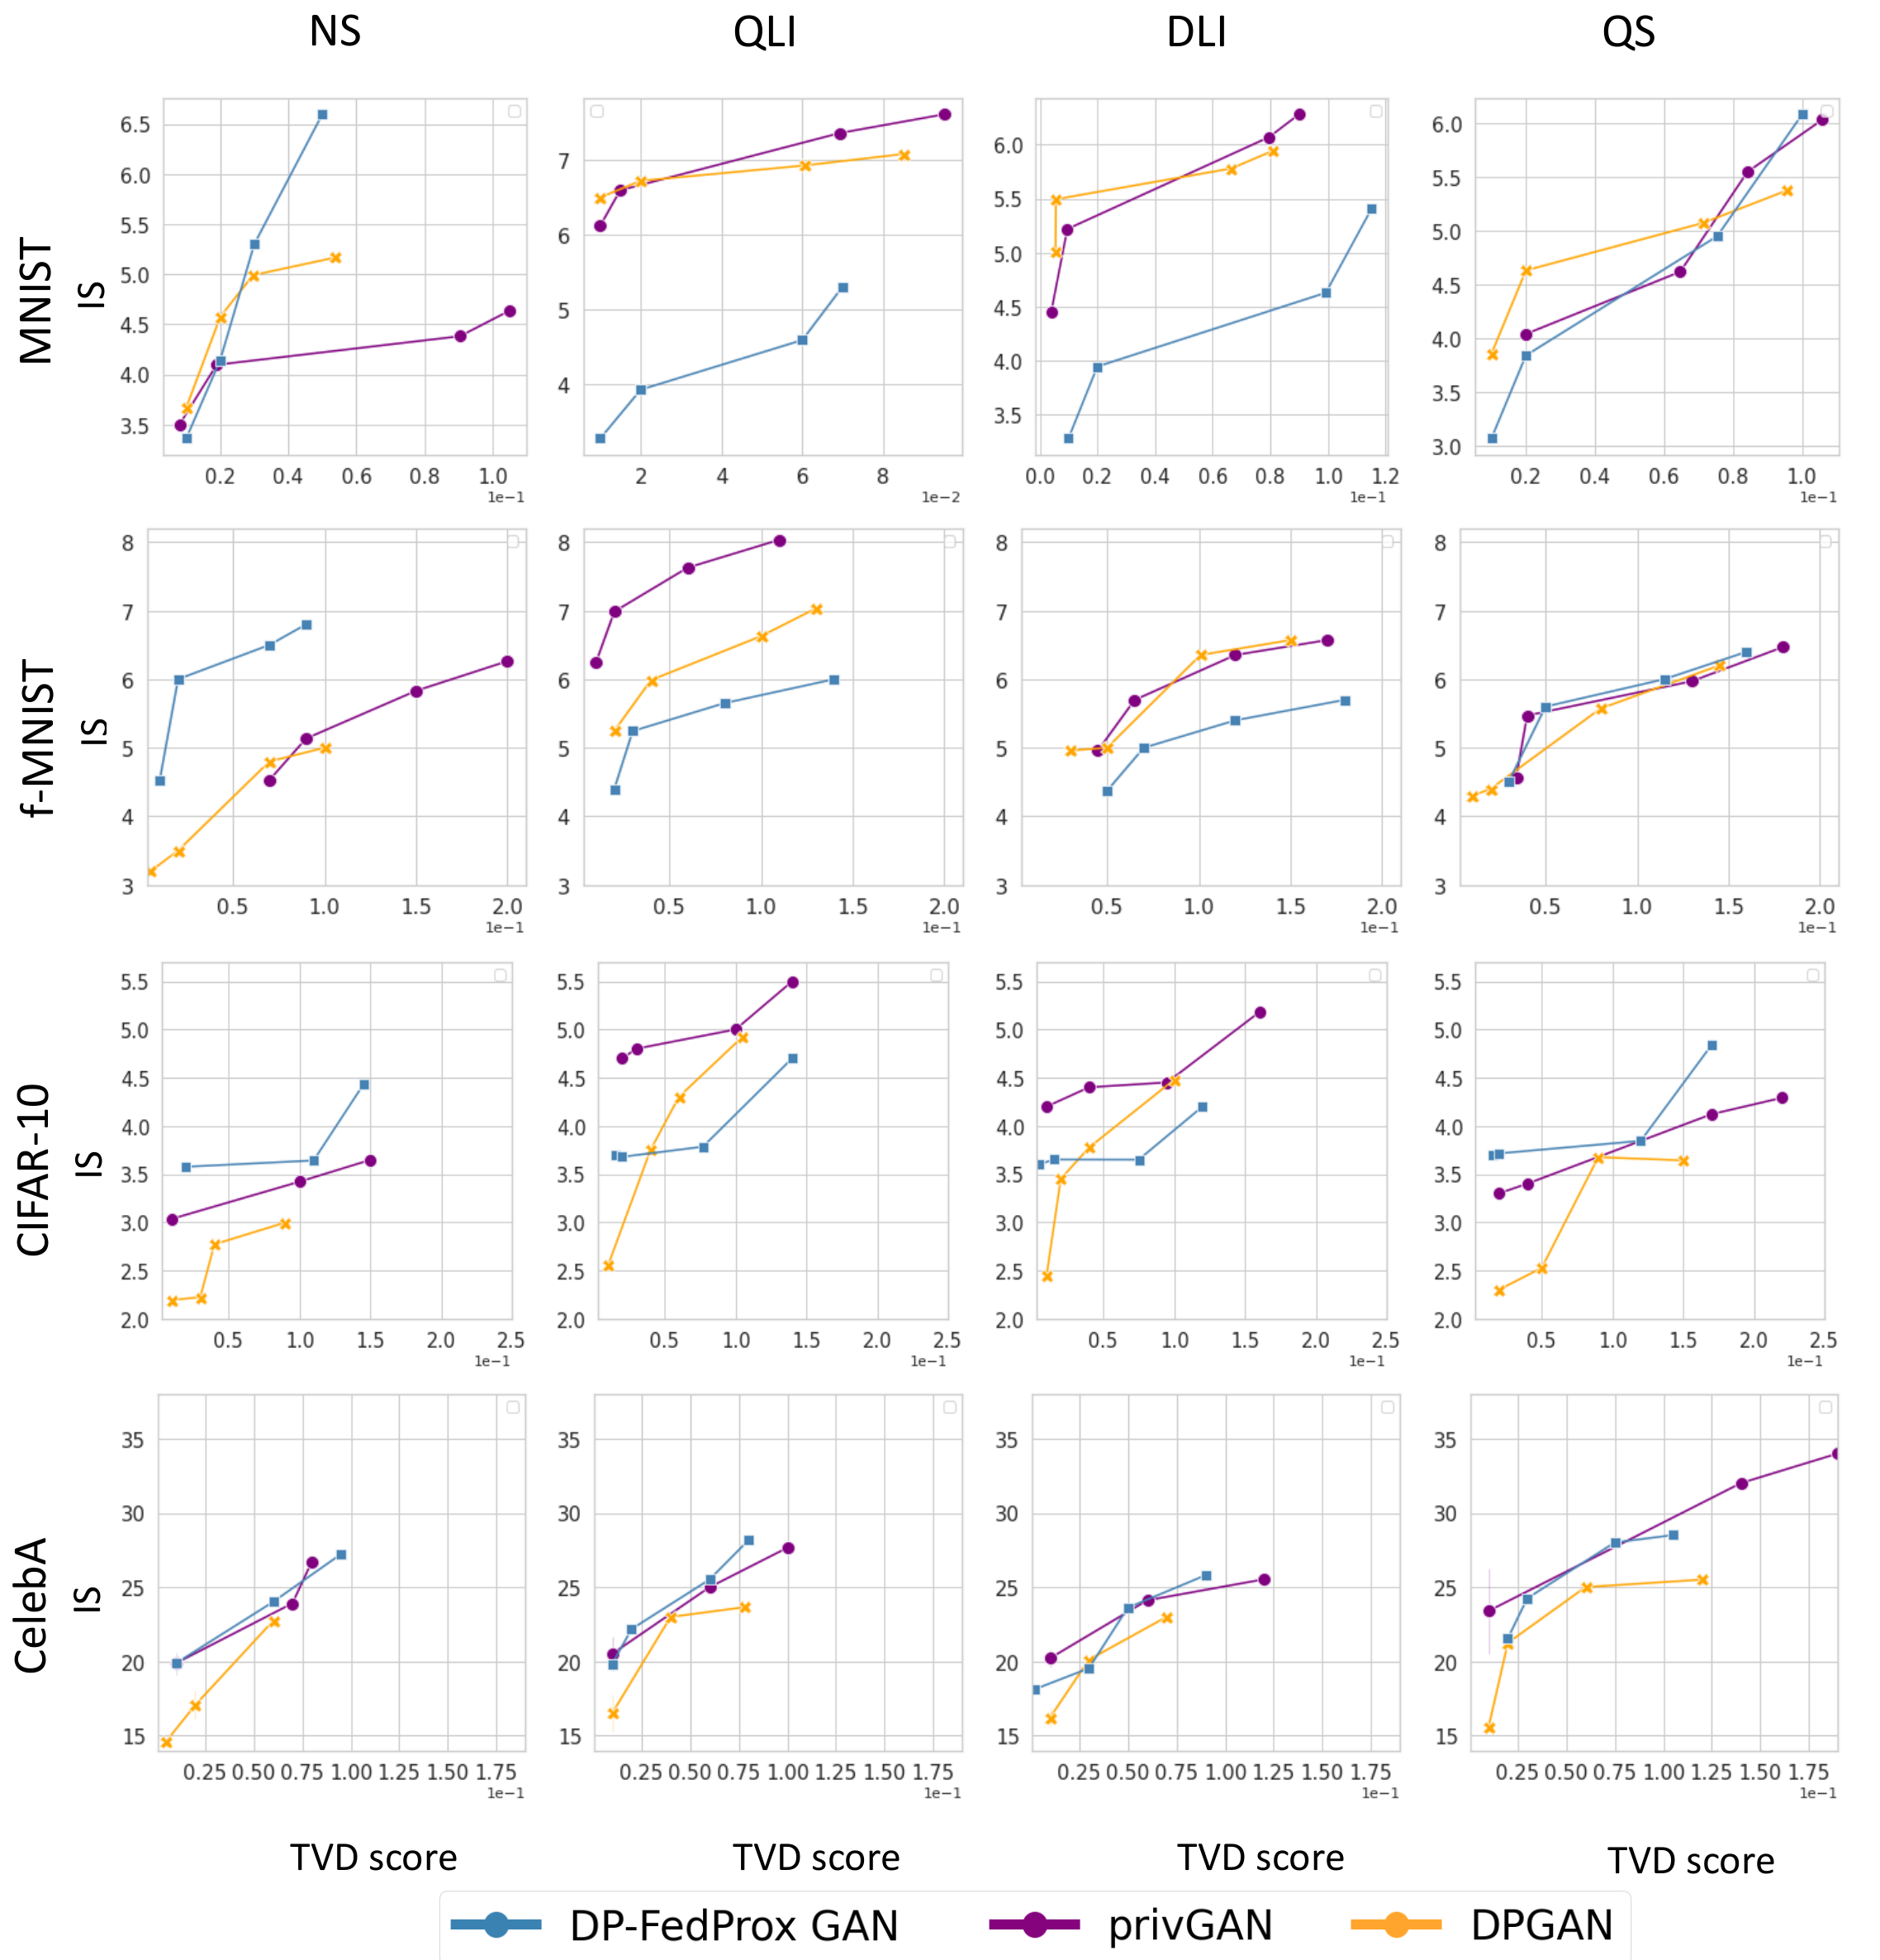
\includegraphics[width=0.8\linewidth]{Plots/varyPrivacy_TVD_IS.png}
 \caption{Privacy vs. Utility: The Figure shows TVD Attack vs Inception Score in privGAN, DPGAN, and DP-FedProx GAN for various privacy parameters.}
 \label{fig:varyPrivacy_MC_IS}
\end{figure}



% \begin{figure}
%  \centering
%  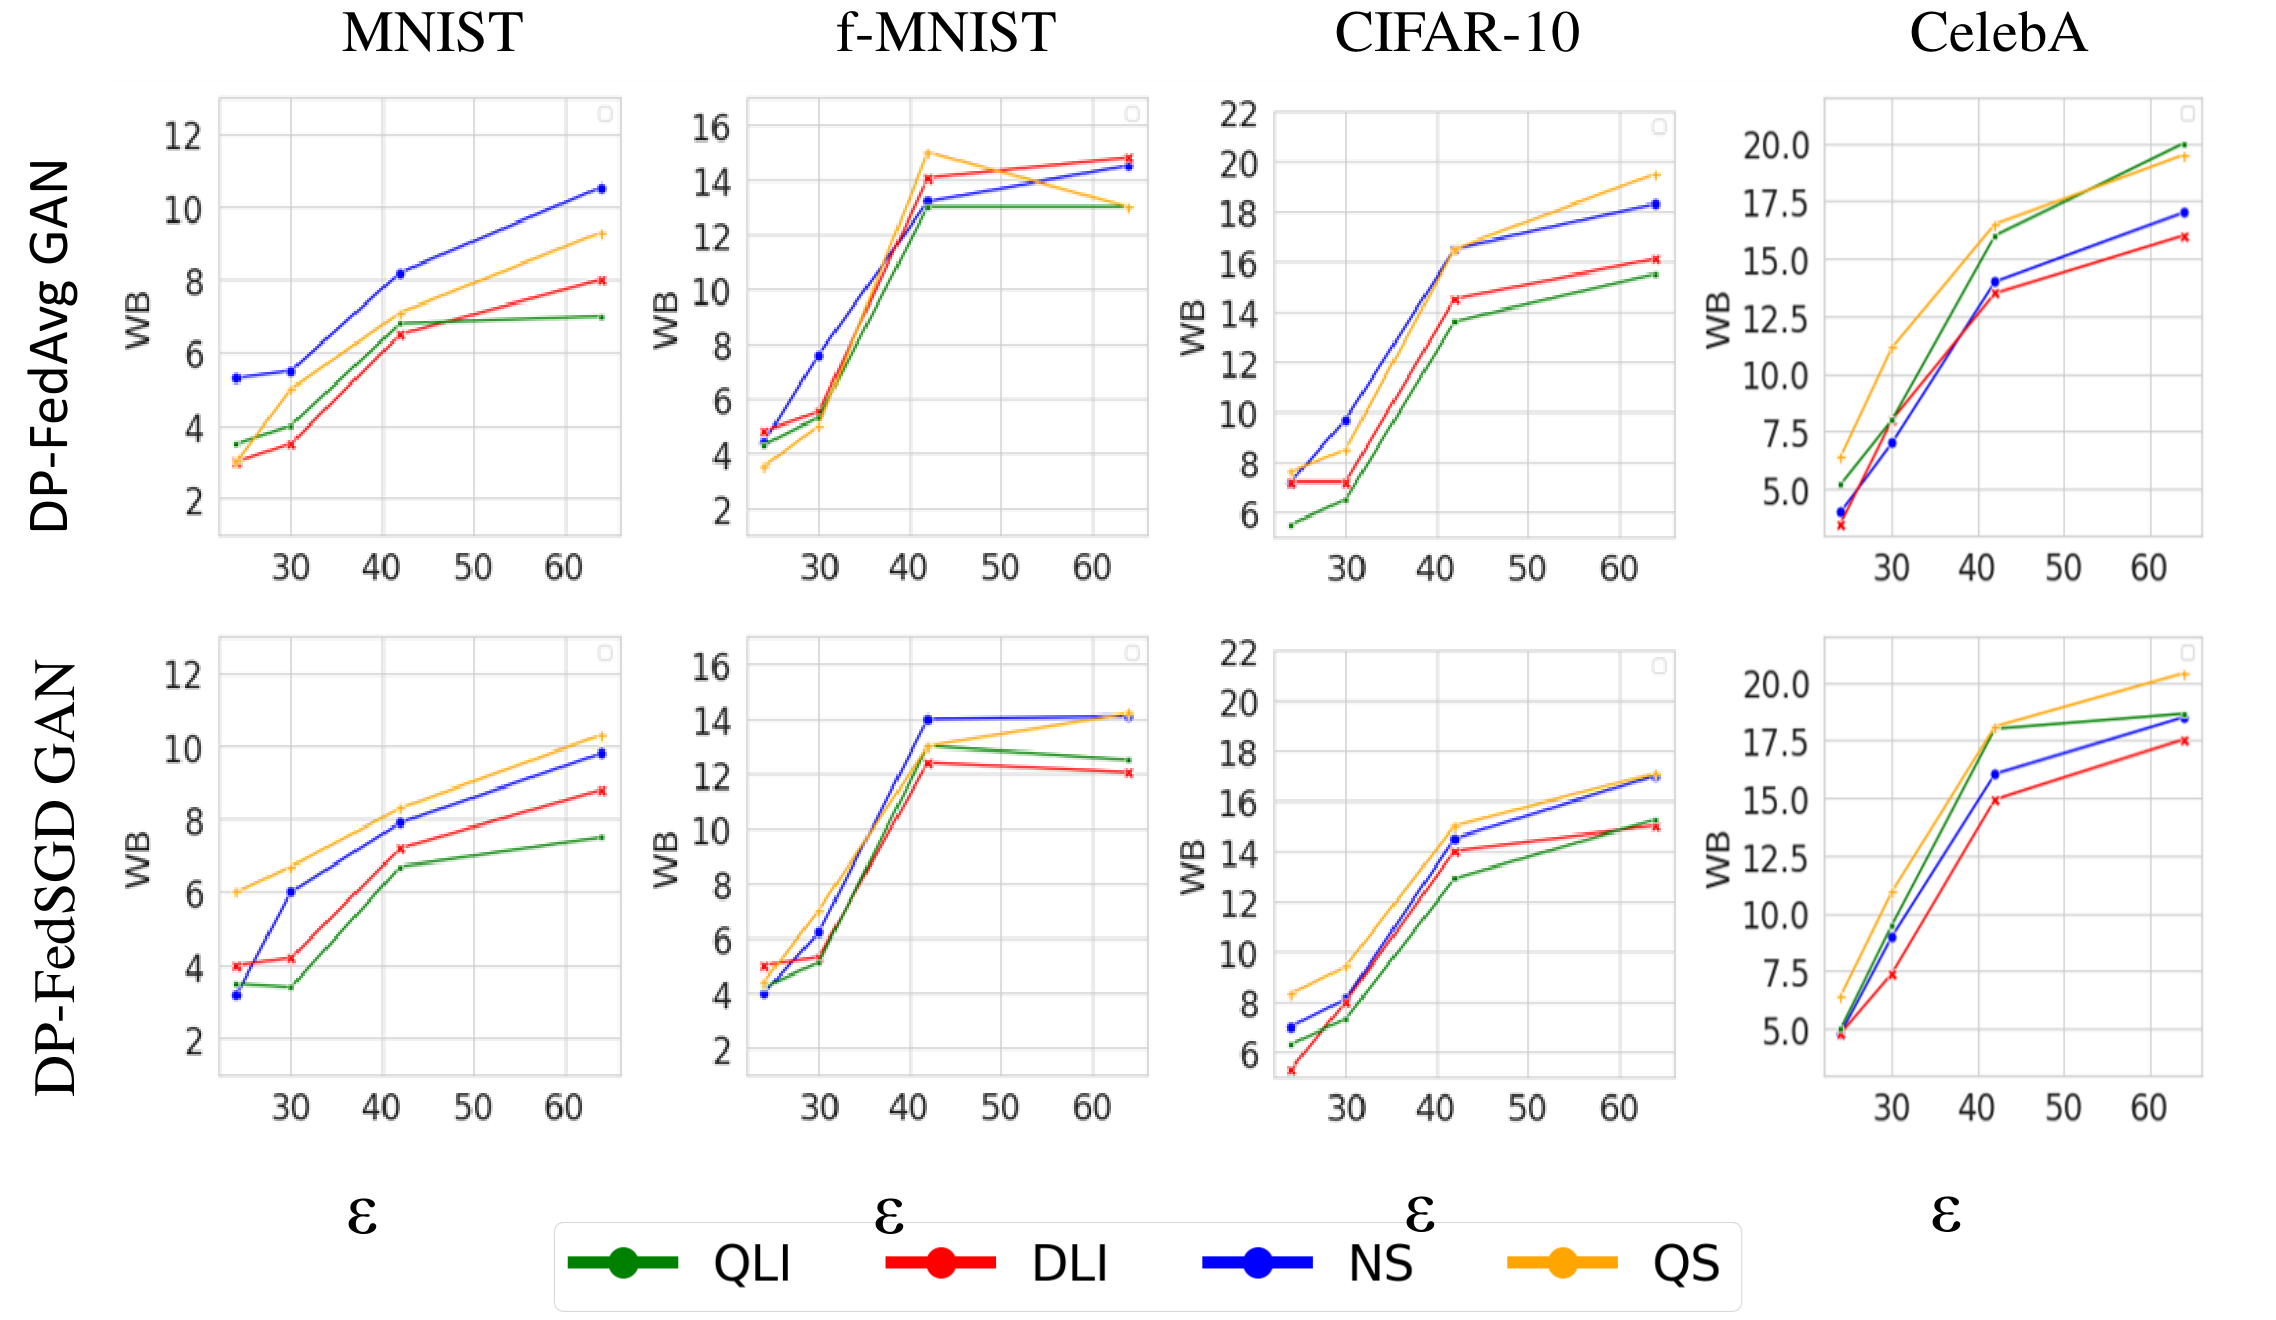
\includegraphics[width=0.8\linewidth]{Plots/vary_privacy_fedsgd_fedavg_WB.png}
%  \caption{Varying Privacy Parameters for WB-Attack: The figure shows WB Attack at various privacy parameters in DP-FedAvg GAN and DP-FedSGD GAN discriminator}
%  \label{fig:vary_privacy_fedsgd_fedavg_WB}
% \end{figure}


% \begin{figure}
%  \centering
%  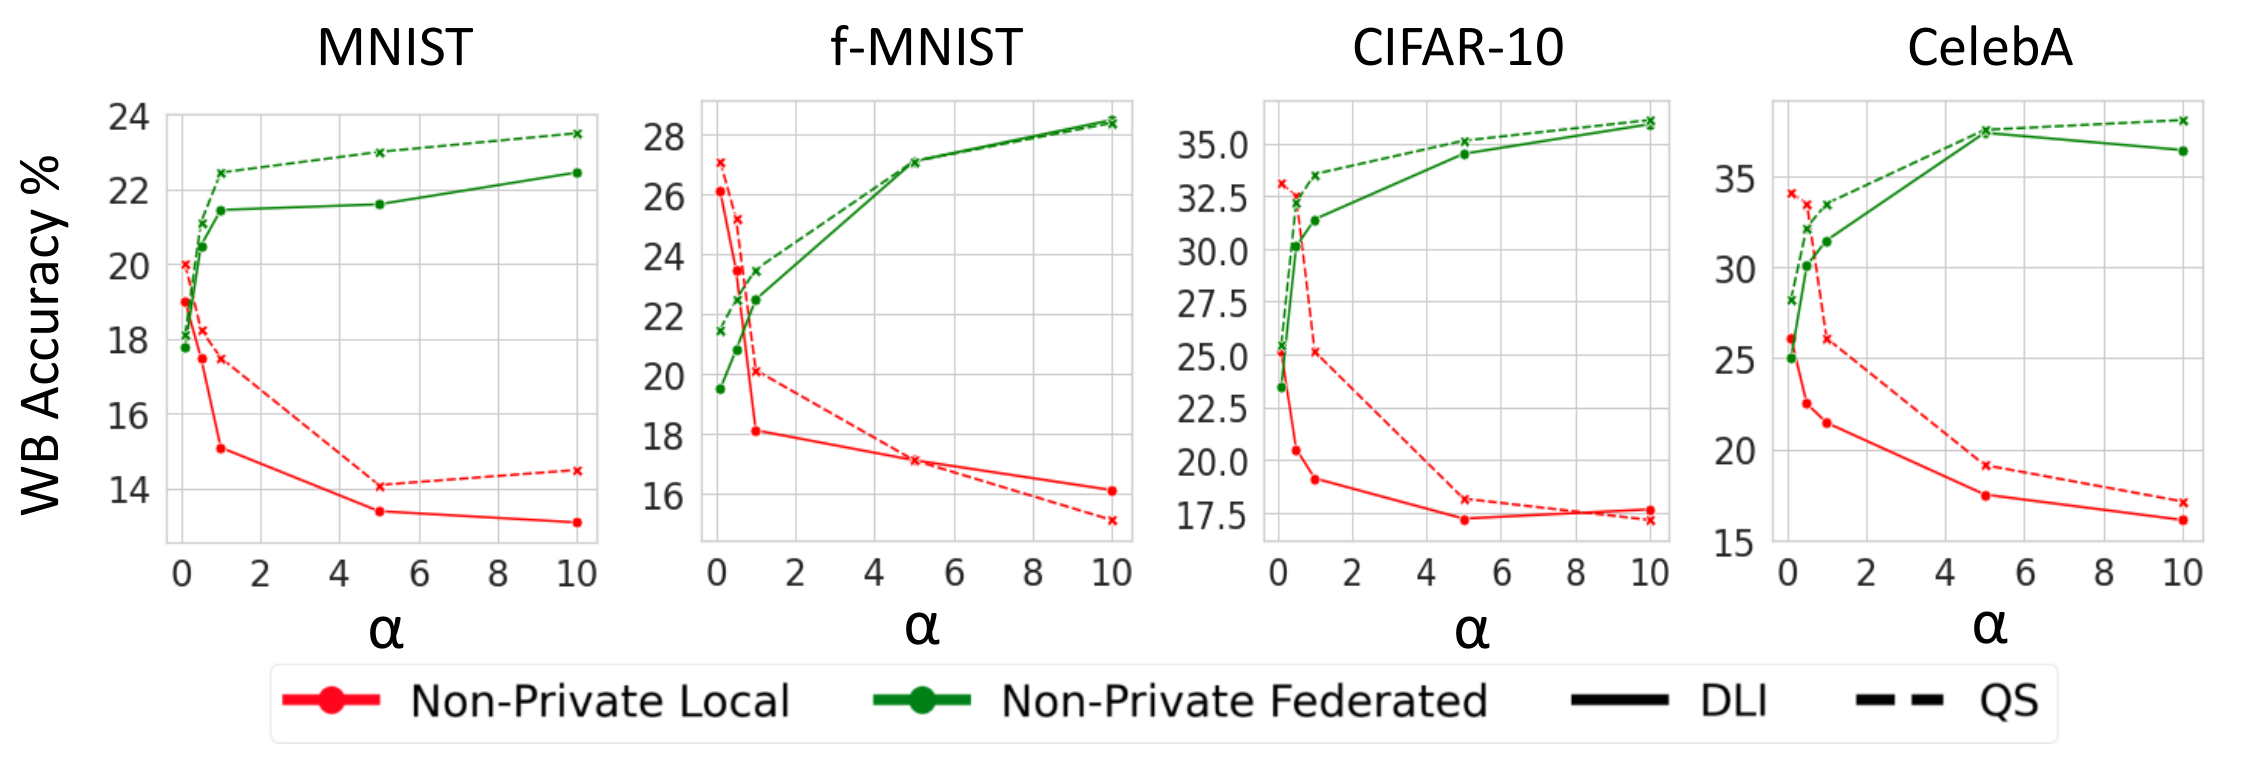
\includegraphics[width=0.8\linewidth]{Plots/nonprivate_vary_alpha_attack.png}
%  \caption{Varying Concentration Parameter for Non-Private Local GANs and Federated GAN: The Figure displays the results of a white-box attack using non-private local GANs and federated GAN with $K=10$ for various concentration parameters.}
%  \label{fig:nonprivate_vary_alpha_attack}
% \end{figure}




% \begin{figure}
%  \centering
%  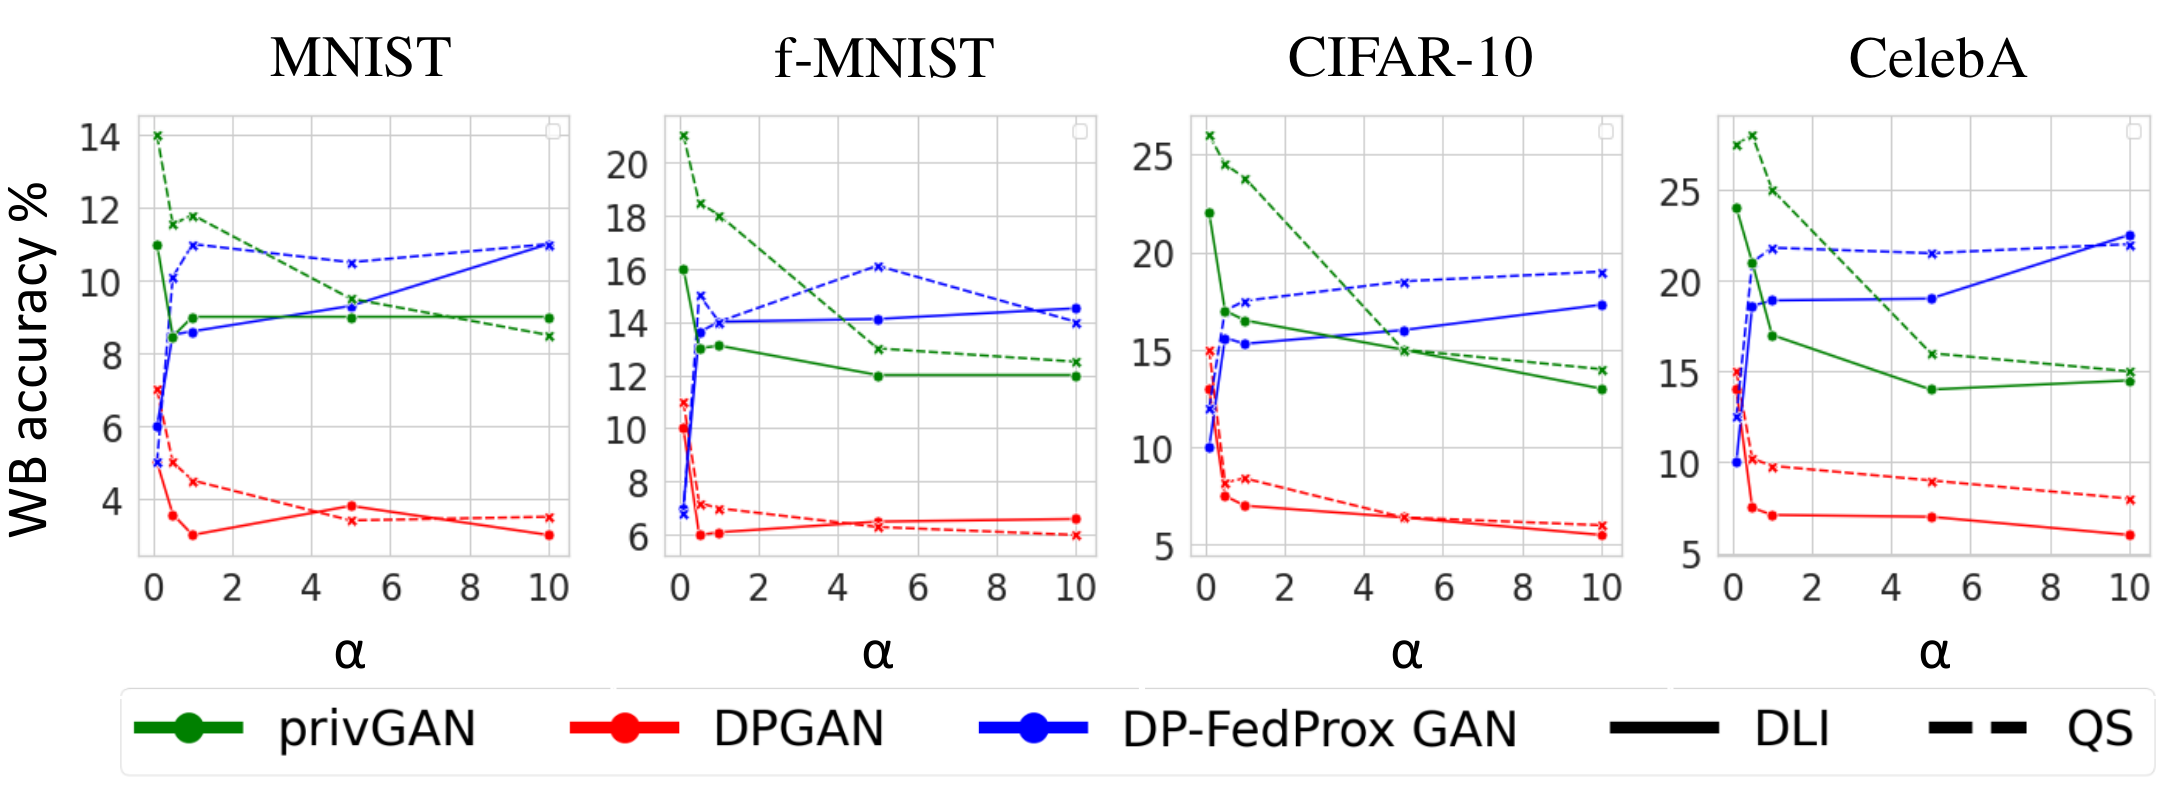
\includegraphics[width=0.8\linewidth]{Plots/vary_alpha_WB.png}
%  \caption{Varying Concentration Parameter: The Figure displays WB Attack at various concentration parameters in privGAN, DPGAN, and DP-FedProx GAN discriminator}
%  \label{fig:vary_alpha_WB}
% \end{figure}








% \begin{figure}
%  \centering
%  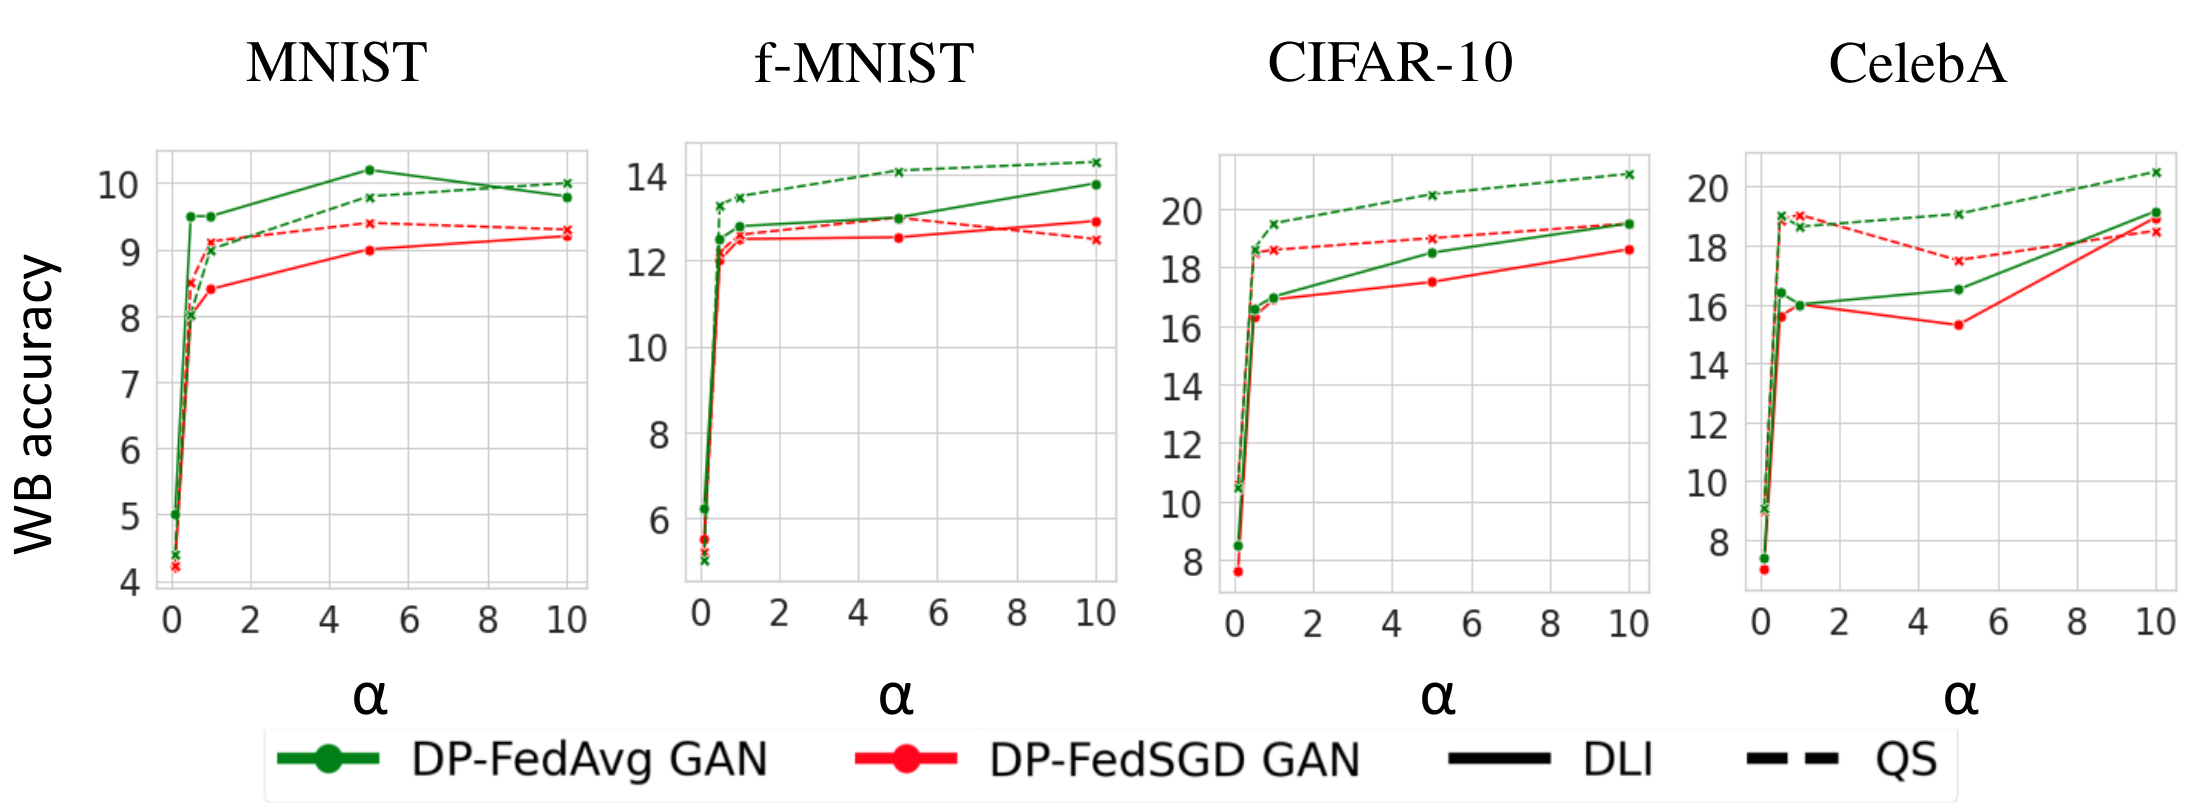
\includegraphics[width=0.8\linewidth]{Plots/vary_alpha_fedsgd_fedavg_WB.png}
%  \caption{Varying Concentration Parameter: The Figure represents WB Attack on discriminator(s) at various concentration parameters in DP-FedAvg GAN and DP-FedSGD GAN. }
%  \label{fig:vary_alpha_fedsgd_fedavg_WB}
% \end{figure}






% \begin{figure}
%  \centering
%  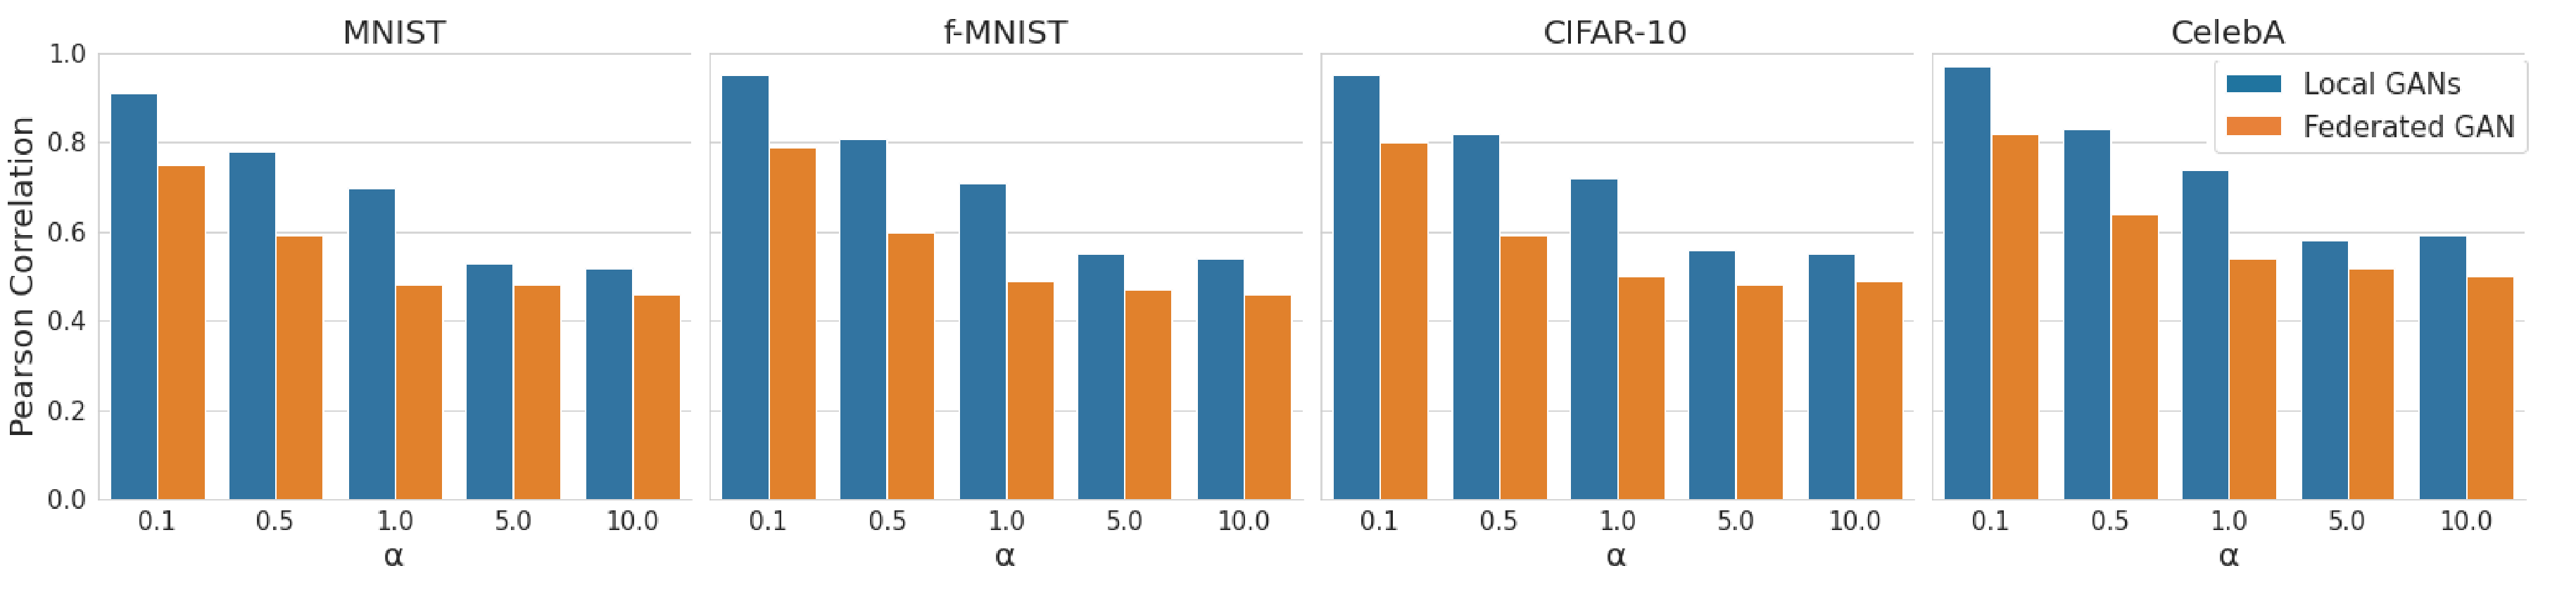
\includegraphics[width=0.8\linewidth]{Plots/WB_alpha_nonprivate.png}
%  \caption{Vary Concentration Parameters in QS distribution: The Figure depicts Pearson correlation $r$ between local data size and local WB accuracy at various concentration parameters $\alpha$ in Local GANs and Federated GAN at $K=10$. }
%  \label{fig:WB_alpha_nonprivate}
% \end{figure}



% \begin{figure}
%  \centering
%  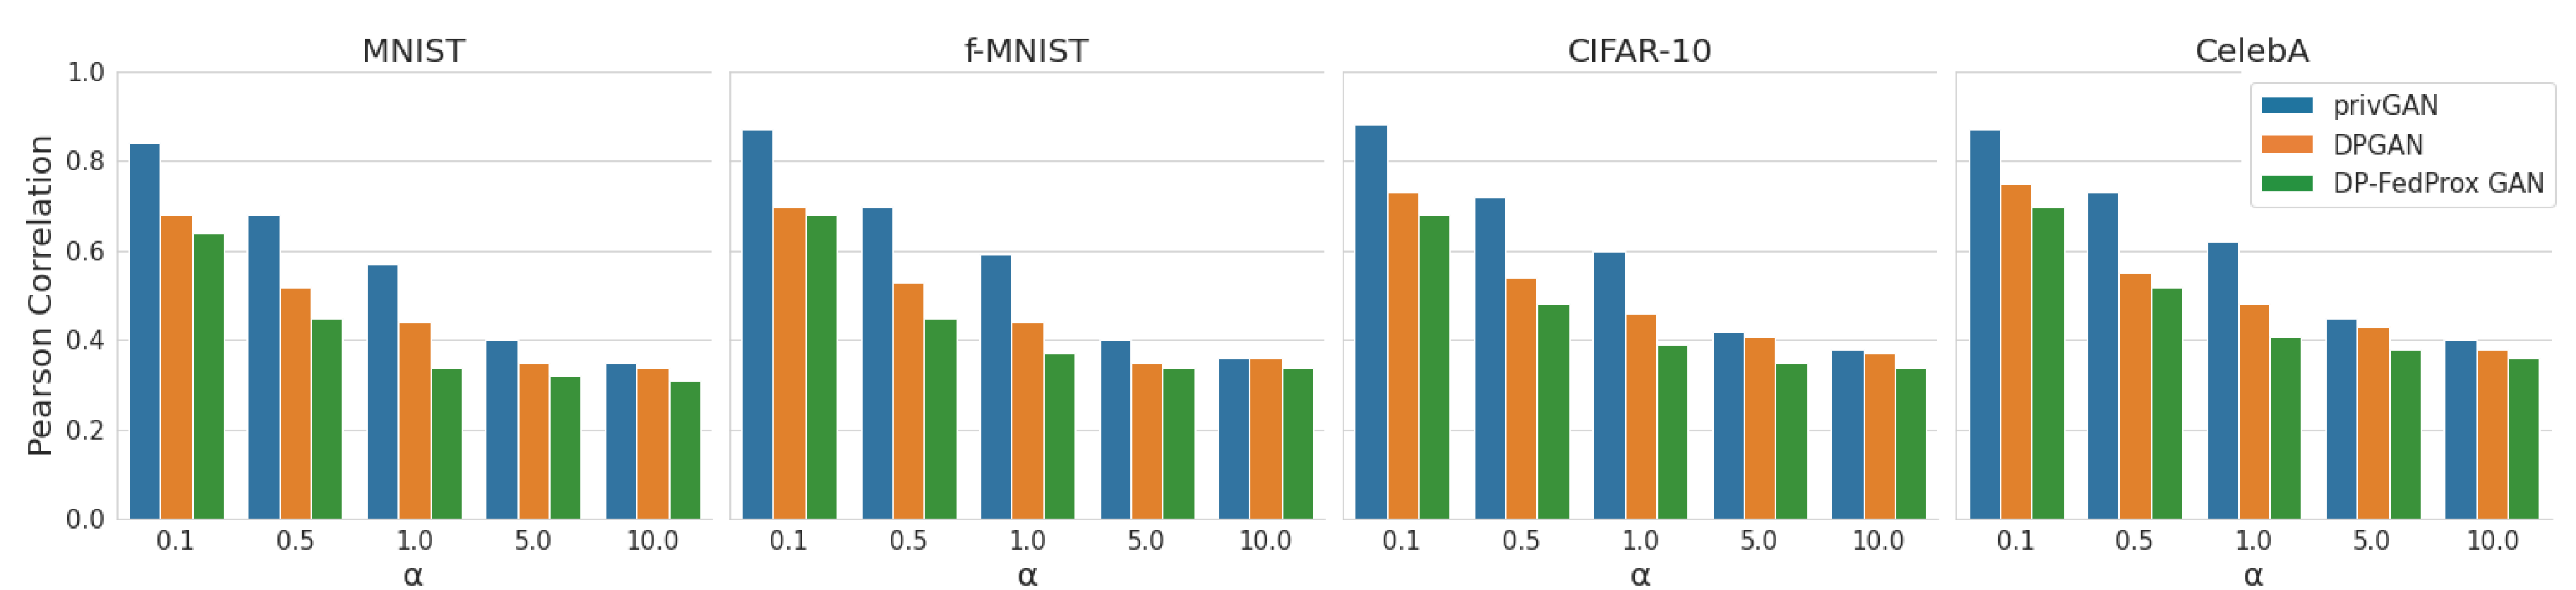
\includegraphics[width=0.8\linewidth]{Plots/Wb_alpha_private.png}
%  \caption{Vary Concentration Parameters in QS distribution: The Figure depicts Pearson correlation $r$ between local data size and local WB accuracy at various concentration parameters $\alpha$ in privGAN, DPGAN, and DP-FedProx GAN.  }
%  \label{fig:Wb_alpha_private}
% \end{figure}


% \begin{figure}
%  \centering
%  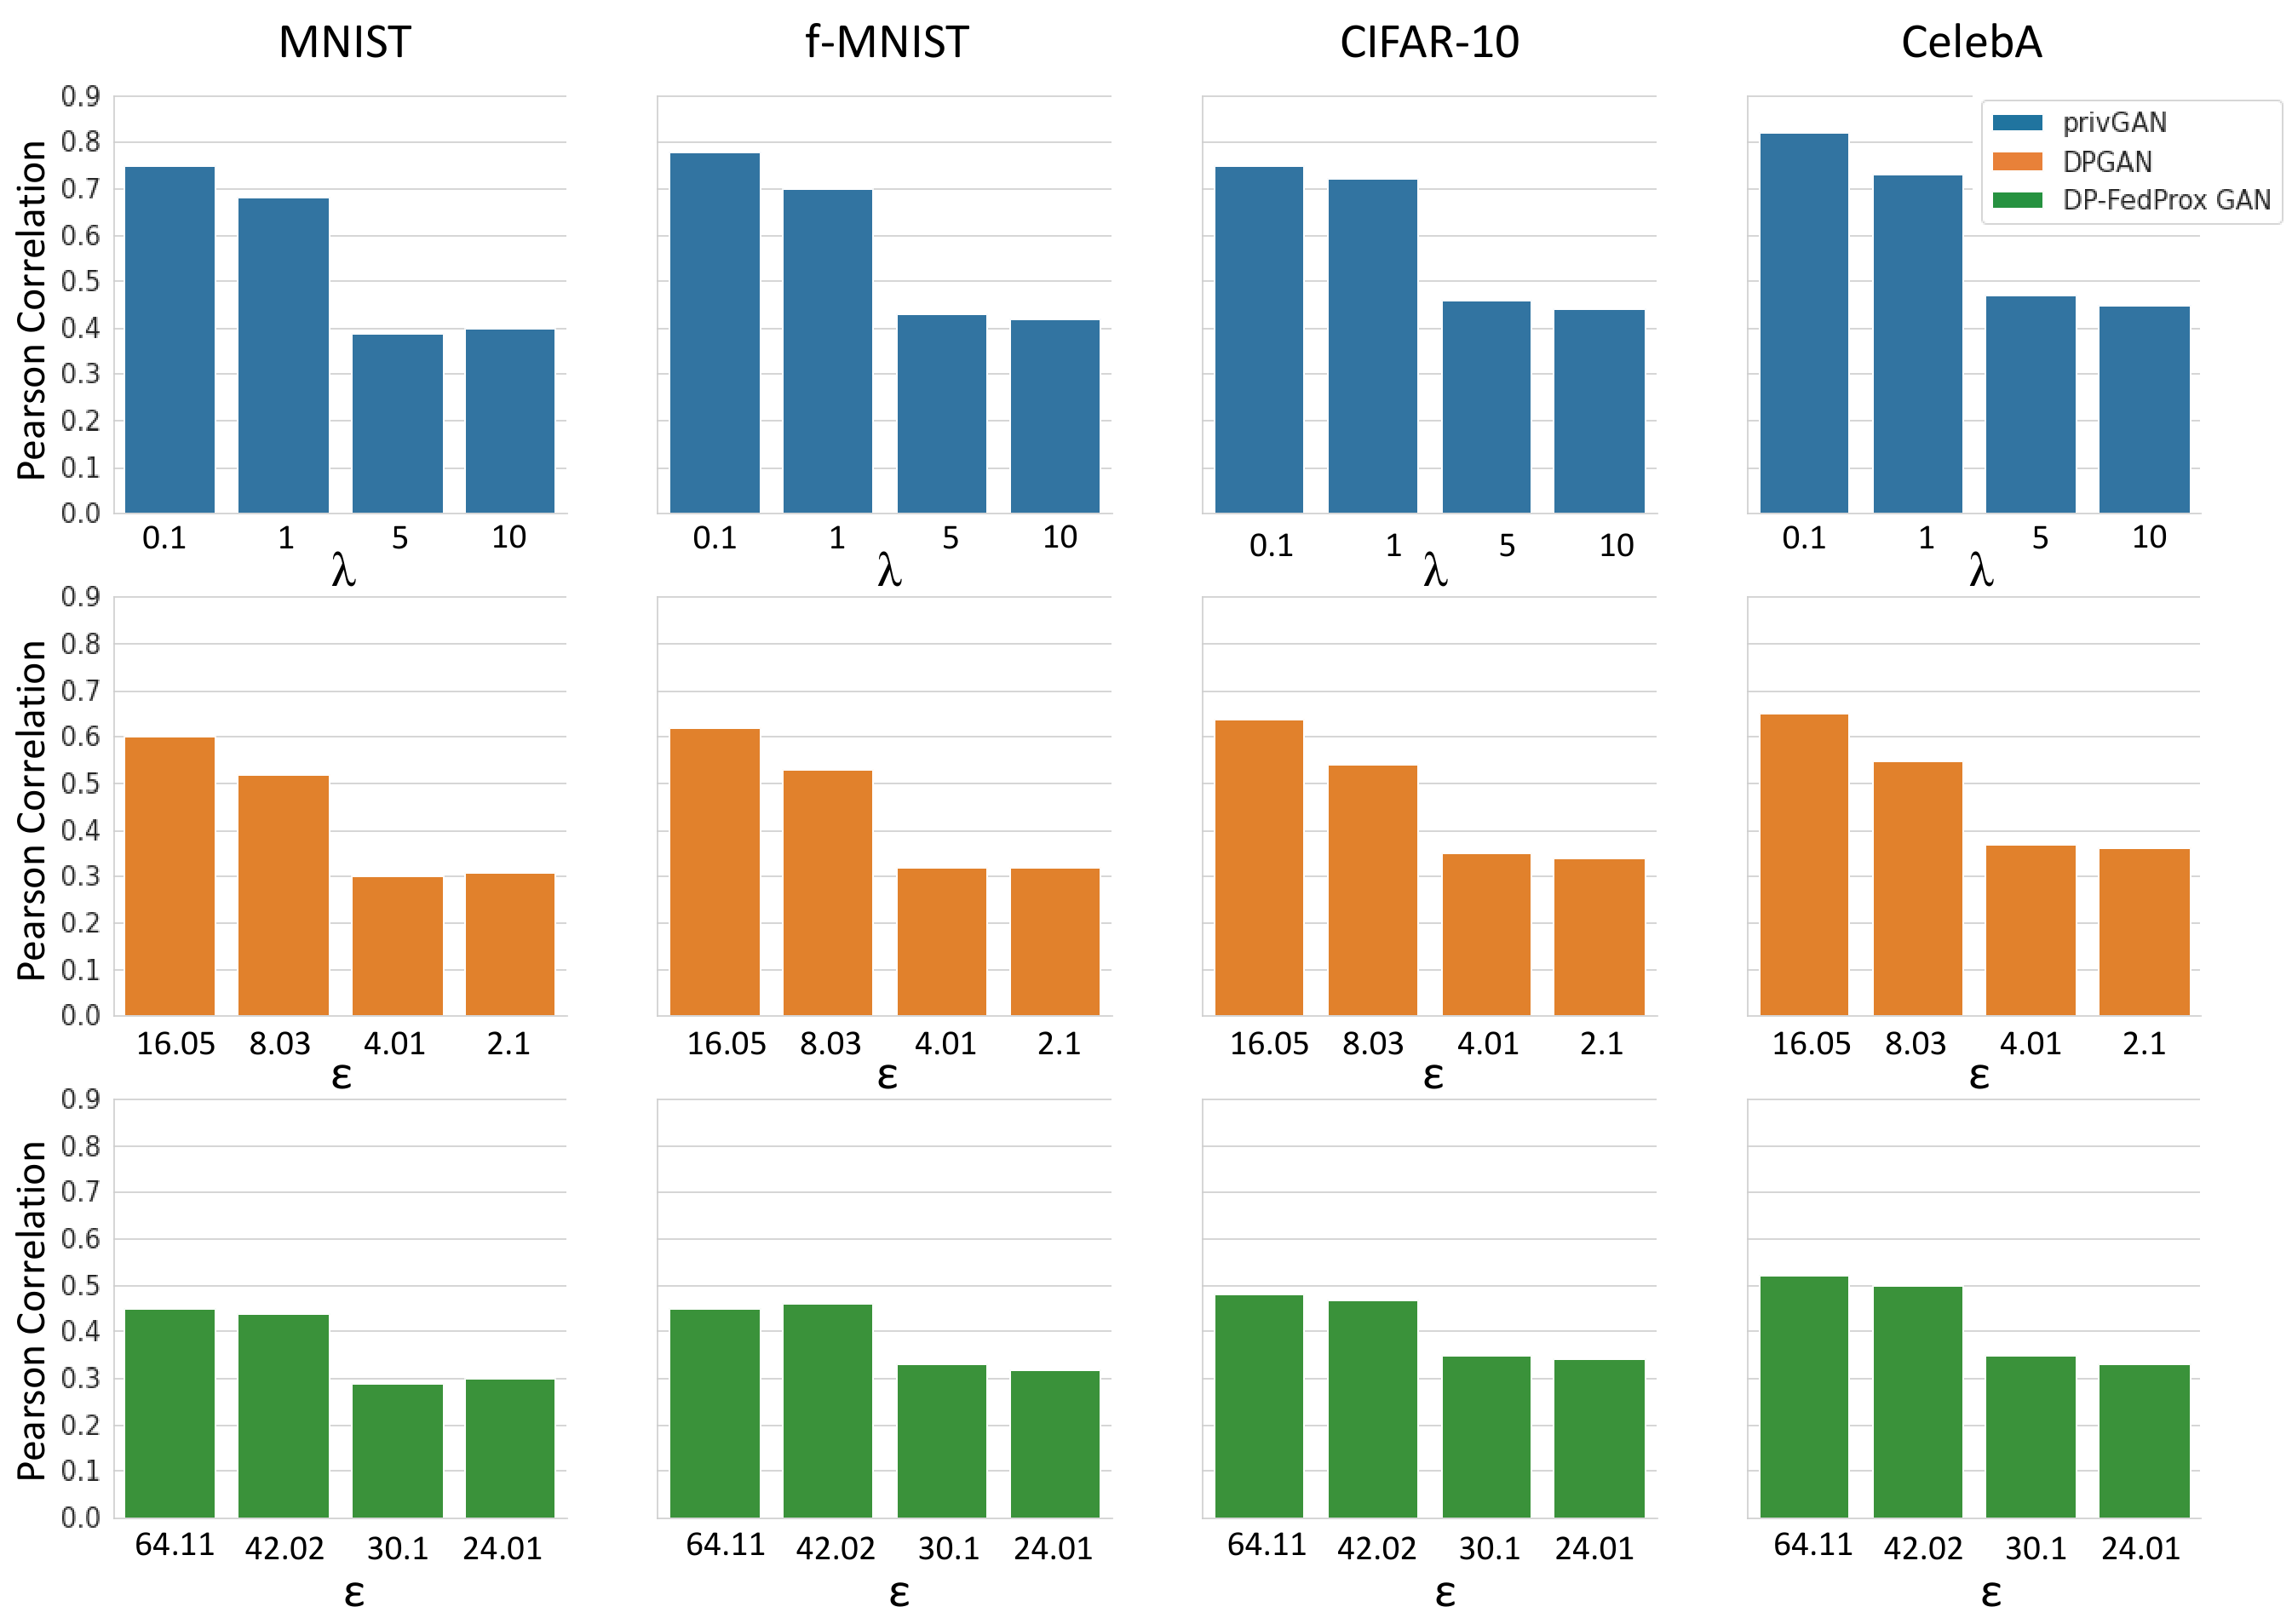
\includegraphics[width=0.8\linewidth]{Plots/Wb_noise_private.png}
%  \caption{Vary Privacy Parameters in QS distribution: The Figure depicts Pearson correlation $r$ between local data size and local WB accuracy at various privacy parameters in privGAN, DPGAN, and DP-FedProx GAN.    }
%  \label{fig:Wb_noise_private}
% \end{figure}









